%%%%%%%%%%%%%%%%%%%%%%%%%%%%%%%%%%%%%%%%%%%%%%%%%%%%%%%%%%%
% PREAMBOLO
%%%%%%%%%%%%%%%%%%%%%%%%%%%%%%%%%%%%%%%%%%%%%%%%%%%%%%%%%%%

 % === Impostazione del documento ==========================
\documentclass[12pt,a4paper,oneside,italian,hidelinks]{book}
\usepackage{setspace}
\onehalfspace

% === Regolazione dei margini =============================\\
%\addtolength{\oddsidemargin}{30pt}
%\addtolength{\evensidemargin}{-30pt}
\usepackage{fancyhdr}
\usepackage{multirow}
\usepackage{rotating}
\usepackage{multicol}
\usepackage[section]{placeins}
\usepackage[usenames,dvipsnames]{color}
\usepackage{appendix}
\usepackage{chngpage}

% === Impostazione dei font ===============================
\usepackage[utf8x]{inputenc}
\usepackage[italian]{babel}
\usepackage[10pt]{type1ec}
\usepackage[T1]{fontenc}
\usepackage{ae}
\usepackage{relsize}
\usepackage{csquotes} 
\usepackage{amsmath}
\usepackage{amsfonts}
\usepackage{mathdots}
\usepackage[colorlinks=true]{hyperref}
\hypersetup{
	bookmarksnumbered=true,
	linkcolor=black,
	citecolor=black,
	urlcolor=black,
}
\usepackage{verbatim}
\usepackage{alltt}

% === Integrazione delle figure ===========================
\usepackage{graphicx}
\graphicspath{{./imgs/}}
\renewcommand{\figurename}{Fig.}
\usepackage{subfigure}

% === Per gli algoritmi ===================================
\usepackage{algorithmicx}
\usepackage[ruled]{algorithm}
\usepackage{algpseudocode}
\usepackage{listings}

% === Per le tabelle ======================================
\usepackage{tabularx}
\usepackage{booktabs}

% === Per gli snippet =====================================
\definecolor{mygreen}{rgb}{0,0.6,0}
\definecolor{mygray}{rgb}{0.5,0.5,0.5}
\definecolor{mymauve}{rgb}{0.58,0,0.82}
\lstset{
  backgroundcolor=\color{white},   % choose the background color; you must add \usepackage{color} or \usepackage{xcolor}
  basicstyle=\footnotesize,        % the size of the fonts that are used for the code
  breakatwhitespace=false,         % sets if automatic breaks should only happen at whitespace
  breaklines=true,                 % sets automatic line breaking
  captionpos=n,                    % sets the caption-position to bottom
  commentstyle=\color{mygreen},    % comment style
  deletekeywords={},			   % if you want to delete keywords from the given language
  escapeinside={\%*}{*)},          % if you want to add LaTeX within your code
  extendedchars=true,              % lets you use non-ASCII characters; for 8-bits encodings only, does not work with UTF-8
  frame=single,                    % adds a frame around the code
  keepspaces=true,                 % keeps spaces in text, useful for keeping indentation of code (possibly needs columns=flexible)
  keywordstyle=\color{blue},       % keyword style
  language=Java,                   % the language of the code
  morekeywords={},            	   % if you want to add more keywords to the set
  numbers=left,                    % where to put the line-numbers; possible values are (none, left, right)
  numbersep=5pt,                   % how far the line-numbers are from the code
  numberstyle=\tiny\color{mygray}, % the style that is used for the line-numbers
  rulecolor=\color{black},         % if not set, the frame-color may be changed on line-breaks within not-black text (e.g. comments (green here))
  showspaces=false,                % show spaces everywhere adding particular underscores; it overrides 'showstringspaces'
  showstringspaces=false,          % underline spaces within strings only
  showtabs=false,                  % show tabs within strings adding particular underscores
  stepnumber=1,                    % the step between two line-numbers. If it's 1, each line will be numbered
  stringstyle=\color{mymauve},     % string literal style
  tabsize=2,                       % sets default tabsize to 2 spaces
  title=\lstname                   % show the filename of files included with \lstinputlisting; also try caption instead of title
}

%%%%%%%%%%%%%%%%%%%%%%%%%%%%%%%%%%%%%%%%%%%%%%%%%%%%%%%%%%%
% TESTO DEL RAD
%%%%%%%%%%%%%%%%%%%%%%%%%%%%%%%%%%%%%%%%%%%%%%%%%%%%%%%%%%%
\begin{document}
	% === Frontespizio ====================================
	%\frontmatter
	\pagenumbering{roman}
	\pagestyle{empty}
	\label{key}%%%%%%%%%%%%%%%%%%%%%%%%%%%%%%%%%%%%%%%%%%%%%%%%%%%%%%%%%%%
% Frontespizio

% vspace serve ad aggiungere extra spazio verticale
% em sta ad indicare la grandezza della lettera M maiuscola

% Large indica una dimensione del font di 14.4 pt
% large indica una dimensione del font di 12 pt
% normalsize indica una dimensione del font di 10 pt

% vfill inserisce sufficiente spazio binaco verticalmente per fare in modo che il
% sopra e il sotto del testo siano allieneati col margine superiore e inferiore
\begin{titlepage}
 \begin{center}
	 \includegraphics[width=3.5cm]{unimol/Unimol.eps}\\
	 \vspace{0.8em}
	 {\Large \textsc{Università degli studi del Molise}}\\
	 \vspace{0.8em}
	 {\Large \textsc{Dipartimento di Bioscienze e Territorio}}\\
	 \vspace{2em}
	 {\normalsize Corsi di Studio in}\\
	 \vspace{1em}
	 {\Large \textsc{Informatica e Sicurezza dei sistemi software}} \\
	 \vspace{1em}
	 {\normalsize Corsi di \textit{Ingegneria del Software} e  \textit{Gestione progetti software}}\\
	 \vspace{5em}
	{\LARGE\textbf{Applicazione \textit{Studenti Unimol}}:} \\
	\vspace{1em}
	{\LARGE\textbf{Requirement Analysis Document (RAD)}} \\
	\vspace{6em}
 \end{center}

\vskip 0.2cm
  \begin{center}
	\begin{tabular}{l c c c c c c l}
	  Docente & & & & & & & Versione 3.0\\[0.2cm]
	  \large{Chiar.mo Prof. Fausto Fasano} & & & & & & & 31/05/2019\\[1cm]
	\end{tabular}
%  \end{center}
\vfill
%\begin{center}
{\normalsize Anno Accademico 2018/2019}
\end{center}
\end{titlepage}
\clearpage
	\newpage
	\thispagestyle{empty}
	\mbox{}

	% === Indice ==========================================
	\setcounter{secnumdepth}{3}
    \setcounter{tocdepth}{2}
	\tableofcontents

	% === Capitoli RAD ===================================
	\pagestyle{plain}
	\newpage
	%\mainmatter
	\pagenumbering{arabic}
	\setcounter{page}{4}
	%%%%%%%%%%%%%%%%%%%%%%%%%%%%%%%%%%%%%h%%%%%%%%%%%%%%%%%%%%%%

\chapter{Dominio del problema}
\label{ref:Introduzione}
Sezione comune a tutti i gruppi: la curerà qualcuno di noi. Non rivolta ai singoli gruppi.
%%%%%%%%%%%%%%%%%%%%%%%%%%%%%%%%%%%%%%%%%%%%%%%%%%%%%%%%%%%

\section{Introduzione al RAD}

\paragraph{}
Questo \textit{Requirement Analysis Document} ha lo scopo di descrivere la fase di raccolta e analisi dei requisiti funzionali, non funzionali e pseudo-requisiti dell'applicazione \textit{Studenti Unimol} quale sistema da sviluppare per gli esami di \textit{Ingegneria del software e laboratorio} e \textit{Gestione progetti software} previsti dai piani di studio del \textit{Corso di studio unificato in Informatica}. Tale documento funge da contratto tra il prof. Fausto Fasano che ha commissionato il sistema e i team di progettazione e sviluppo che lo realizzeranno. Esso fornisce una panoramica astratta del sistema che gli studenti si accingeranno ad implementare.

\section{Scope}

\paragraph{}
Questo progetto ha come scopo quello di realizzare una App ufficiale per l’Università degli Studi del Molise. L’obiettivo è quello di rendere disponibile, agli studenti universitari, i principali servizi di Ateneo attraverso un’applicazione completa ed esaustiva.
In primo luogo, dal punto di vista informativo ed organizzativo, il sistema deve essere capace di focalizzarsi sull’esigenza comune agli studenti di accedere velocemente alle informazioni e ai dati afferenti al proprio Piano di Studio. In tal modo, lo studente può monitorare in modo agevole ed intuitivo tutto ciò che attiene al proprio percorso universitario e alle principali attività svolte all'interno dell'Ateneo.

La tecnologia usata facilita estremamente l'utilizzo dell'applicazione. Si tratta di un’app ibrida multipiattaforma, che permette di avere alte performance su ciascun dispositivo mobile, in particolar modo su smartphone \textit{iOS} e \textit{Android}.  L’app supporta funzionalità di base ma anche funzionalità avanzate, le quali garantiscono un servizio aggiuntivo per gli studenti che decidono di utilizzarla. Lo studente può visualizzare tutti i suoi dati universitari e compiere una serie di attività, accedendo con le sue credenziali del portale \textit{Esse3} alla propria area personale. Tra le funzionalità avanzate, introdotta nell'anno accademico 2018/2019, è presente un servizio di messagistica instantaneo.
L'idea di base è quella di fornire un sistema di comunicazione semplice ed affidabile, evitando la trasmissione di informazioni personali, quali i contatti personali, come numero di telefono ed email, di docenti e studenti.
Le chat sono create automaticamente in base alla \textit{Coorte accademica} e ai relativi \textit{corsi} e sono manutenute per un periodo limitato di tempo. La chat verrà abilitata per ciascuno studente o docente nel momento in cui egli fa il login nell’\textit{app}.


\section{Contesto e panoramica del sistema}
Il corso di \textit{Ingegneria del software e laboratorio} all'\textit{Università degli Studi del Molise} prevede la suddivisione degli studenti in gruppi di lavoro ai quali è chiesto di progettare, documentare e sviluppare alcune funzionalità interne all'applicazione \textit{Studenti Unimol} utilizzata dagli studenti per la gestione semplificata della loro carriera accademica. Sarà rilasciata una versione aggiornata di quella attuale previa revisione della versione già esistente. Essa sarà resa disponibile a tutti gli studenti regolarmente iscritti all'\textit{Università degli Studi del Molise}.

\section{Manager di progetto e sviluppatori}

\paragraph{}
L'app \textit{Studenti Unimol} è stata documentata e implementata nel 2017 dagli studenti del corso di \textit{Ingegneria del Software}, coordinati da gruppi di manager del corso magistrale in \textit{Sicurezza dei sistemi software}, operanti nell'ambito dell'insegnamento di \text{Gestione progetti software}. Successivamente l'applicazione è stata manutenuta dal prof. Fausto Fasano, il quale, nel 2019, ha chiesto agli studenti di triennale e magistrale di manutenere e far evolvere l'attuale applicazione per produrre la versione 3.0. Ogni team è supervisionato da alcuni manager che si occuperanno della comunicazione e dell'organizzazione dell'intero progetto, coordinando i gruppi a loro assegnati e gestendo le relazioni orizzontali tra i gruppi che lavorano in parallelo su funzionalità diverse dell'app. \\

\textbf {Gruppo 1 - Funzionalità: piano di studi, appelli, materiale didattico} \\ \\
\textbf{Manager} \\
Fantini Martina (PM), Fierro Fabiana (PM), Varriano Giulia (QM), Mastropaolo Antonio (SM). \\
\textbf{Ingegneri del software} \\
Caserio Walter, Ciaramella Giovanni, Daniele Raffaele, De Turris Antonio, Discenza Christian, Fagnano Stefano, Iannotti Carmine,  Muccigrosso Marco, Russodivito Marco, Tata Giancarlo. \\

\textbf{Gruppo 2 - Funzionalità: gestione notifiche e gestione orario} \\ \\
\textbf{Manager} \\
Piedimonte Massimo (PM), Placella Davide (PM), La Rocca Piera Elena (QM), Polisena Alessandro Bruno (QM), Di Tommaso Fabio (SM). \\
\textbf{Ingegneri del software} \\
Armenti Carmen, Buro Martina, Cocozza Nicola, Discenza Silvia, Lucchetti Roberto, Mazzocco Giuseppina, Schiavone Raffaele, Siravo Luca, Spina Chiara, Varrati Angelo Gino. \\

\textbf {Gruppo 3 - Funzionalità: previsione della media} \\ \\
\textbf{Manager} \\Crincoli Giuseppe (PM), Fabrizio Emilio (PM), D'Ercole Giovanna (QM), Di Cristino Gianluca (SM). \\
\textbf{Ingegneri del software} \\Cancelliere Alessandro, Di Pilla Francesco, Maglioli Raffaele, Marzullo Alessio, Placella Andrea, Stefanelli Vincenzo, Venditti Giorgio.\\

\textbf {Gruppo 4 - Funzionalità: news} \\ \\
\textbf{Manager} \\
Fausto Fasano. \\ \\ \\ \\

\textbf {Gruppo 5 - Funzionalità: rubrica} \\ \\
\textbf{Manager} \\
Carnevale Filippo (PM), Marinaro Tiziano (QM), Tortola Domenico (SM). \\
\textbf{Ingegneri del software} \\
Ciardiello Gabriele, Pizzi Mario, Vitiello Giò. \\

\textbf{Gruppo 6 - Funzionalità: chat per studenti e docenti con annesso pannello di amministrazione} \\ \\
\textbf{Manager} \\
\textbf{} 
Giovanni Rosa (PM), Michele Guerra (QM), Angelo Iallonardi (SM). \\
\textbf{Ingegneri del software } \\
Daniele Albanese, Antonio Antenucci, Mattia Ciccaglione, Andrea D'Aguanno, Antonio De Santis,  Francesco Di Rito, Gianluca Farinaro, Antonio Fratianni, Emanuela Guglielmi, Gaia Iannone, Aldo Palombo, Marica Principe, Federico Zappone.

\clearpage
\section{Glossario}

\paragraph{}
Di seguito è riportata una tabella degli acronimi e dei termini tecnici utilizzati nel documento:

\begin{table}[!h]
\begin{tabular}{p{1.5in}|p{4in}} \\
	{\bf Termine o sigla} & {\bf Descrizione} \\ \hline
	\textbf{RAD} & \textit{Requirement Analysis Document}, documento di analisi dei requisiti. \\
	\textbf{Attore} &  Entità esterna al sistema che interagisce con
	esso. In questo documento la definizione degli attori viene trattata al paragrafo \ref{sec:attori} \\
	\textbf{Modello di workflow} & Modello del flusso di lavoro: indica il modello di sistema che viene utilizzato dagli sviluppatori durante la fase di analisi dei requisiti e implementazione del sistema. \\
	\textbf{Scenario} & Singola istanza di un caso d’uso. Descrive concretamente una situazione ipotetica che potrebbe verificarsi all'avverarsi di un caso d’uso. \\
	\textbf{Caso d'uso} & Flusso di eventi che coinvolge il sistema e alcuni attori che si genera quando  un attore interagisce con il sistema e, poiché sono soddisfatte delle condizioni di ingresso e dei vincoli, vengono eseguite alcune azioni affinché il flusso termini con una o più condizioni d’uscita. \\
	\textbf{Diagramma di sequenza} & Rappresenta un diagramma che serve per descrivere uno scenario in cui le scelte o i flussi alternativi sono rappresentati tramite un pannello di "alt". In particolare servono per dare una visione specifica del flusso degli eventi a livello applicativo. \\
	\textbf{Screen mockup} & Rappresenta un prototipo dell’interfaccia che il sistema presenterà allo studente e permette al lettore di immaginare la veste grafica dell’applicazione e l’implementazione di uno specifico caso d’uso. \\
\end{tabular}
\end{table}
\clearpage
	%%%%%%%%%%%%%%%%%%%%%%%%%%%%%%%%%%%%%%%%%%%%%%%%%%%%%%%%%%%

\chapter{Analisi dei requisiti - gruppo 1}
\label{ref:requisiti1}

%%% Il gruppo 1 scriverà qui i suoi requisiti funzionali e non funzionali %%%

\section{Requisiti funzionali}

%%%%%%%%%%%%%%7.1.1 Gestione piano di studio%%%%%%%%%%%%%%%%%
\subsection{Gestione piano di studio}
\paragraph{} 
L’app dovrà mostrare i corsi previsti dal piano di studio dello studente permettendo la visualizzazione di tutti i corsi ad esso afferenti evidenziando quelli per cui l’esame è stato sostenuto e quelli per cui l’esame è da sostenere. Per ogni corso saranno inoltre visualizzati i relativi dettagli, come il numero di CFU, la valutazione in trentesimi oppure eventuale idoneità. Lo studente potrà effettuare le operazioni di ricerca, filtro e ordinamento dell'elenco dei corsi e potrà scegliere se memorizzare nello \textit{storage} le sue preferenze oppure resettarle. Il sistema richiederà i dati aggiornati al sincronizzatore, il quale si occuperà di salvarli nello \textit{storage} dell’app.
%%%%%%%%%%%7.1.2 Visualizza dettagli corso%%%%%%%%%%%%%%%%%%%
\subsection{Visualizza dettagli corso}
\paragraph{} 
L’app dovrà mostrare informazioni relative a ciascun corso cliccando sullo stesso nella sezione carriera. Selezionando la voce \textit{dettagli}, l’app mostrerà allo studente, per ogni corso, il/i docente/i responsabile/i dell’insegnamento, il numero di CFU, l’anno accademico in cui viene frequentato il corso ed i suoi contenuti. Da tale sezione, inoltre, si potranno raggiungere le interfacce del materiale didattico e dell’elenco appelli. Selezionando un corso il cui esame è già stato sostenuto sarà, invece, possibile ottenere anche informazioni relative alla data in cui è stato svolto, alla data in cui è stato verbalizzato ed il voto ottenuto. Il sistema richiederà i dati aggiornati al sincronizzatore, il quale si occuperà di salvarli nello \textit{storage} dell’app.
%%%%%%%%%%%7.1.3 Gestione materiale didattico %%%%%%%%%%%%%
\subsection{Gestione materiale didattico}
\paragraph{} 
L’app mostrerà l’elenco dei file relativi ad un corso selezionato, dopo aver richiesto i dati al sincronizzatore, averli ricevuti e salvati nello \textit{storage} dell’applicazione. Per visualizzare un file selezionato dalla lista, questo dovrà essere prima scaricato all’interno dello \textit{storage} dell’app: in tal caso, il file potrà essere aperto e visualizzato. Nel caso in cui il file selezionato fosse stato precedentemente scaricato sarà possibile eliminarlo, altrimenti quest’ultima notificherà allo studente l’assenza del file nello \textit{storage} e gli chiederà se è intenzionato a scaricarlo. Se lo studente sceglierà di scaricare un file, il sistema richiederà i dati aggiornati al sincronizzatore, il quale si occuperà di salvarli nello \textit{storage} dell’app.
%%%%%%%%%%%%%%%%%% 7.1.4 Gestione appelli %%%%%%%%%%%%%%%%%%%
\subsection{Gestione appelli}
\paragraph{} 
L’app dovrà mostrare l’elenco degli appelli disponibili richiedendoli al sincronizzatore e salvando nello \textit{storage} i dati ricevuti: lo studente potrà prenotarsi a uno specifico appello tra quelli visualizzati, che saranno solo quelli prenotabili. Lo studente potrà effettuare le operazioni di ricerca, filtro con parola chiave e ordinamento dall'elenco di appelli disponibili e scegliere se memorizzare nello \textit{storage} le sue preferenze oppure resettarle. Il sistema richiederà i dati aggiornati al sincronizzatore, il quale si occuperà di salvarli nello \textit{storage} dell’app. Lo studente, selezionando una data di appello, potrà effettuare una prenotazione, la quale verrà inserita dal sistema nell’elenco degli appelli prenotati. La prenotazione potrà essere annullata fino a cinque giorni prima della data di esame.


\section{Requisiti non funzionali}

%%%%%%%%%%%%% 7.2.1 Usabilità e user experience %%%%%%%%%%%%%
\subsection{Usabilità e \textit{user experience}}
\paragraph{} 
L’app dovrà essere semplice da utilizzare per agevolare ogni studente dell’\textit{Università degli Studi del Molise} nel monitoraggio della propria carriera universitaria. L’applicazione, inoltre, sarà dotata di un’interfaccia \textit{user friendly} per essere utilizzata e compresa con facilità. A tal proposito la prima volta che l’app sarà aperta verrà mostrato un breve tutorial che offrirà una panoramica veloce riguardante le funzionalità principali. L’app mostrerà messaggi di errore utilizzando una grafica piacevole.

%%%%%%%%%%%%% 7.2.2 Affidabilità %%%%%%%%%%%%%
\subsection{Affidabilità}
\paragraph{} 
L’app dovrà essere fruibile anche in assenza di connessione mostrando gli ultimi dati salvati nello \textit{storage}. L’app non dovrà avere arresti casuali e improvvisi, ma dovrà restituire dati esatti e non alterati.

\section{Pseudorequisiti e vincoli}
\paragraph{Sostituire con gli pseudorequisiti e vincoli da rispettare \\}
Lorem ipsum dolor sit amet

\clearpage

	\input{Requisiti_gruppo2.tex}
	%%%%%%%%%%%%%%%%%%%%%%%%%%%%%%%%%%%%%%%%%%%%%%%%%%%%%%%%%%%

\chapter{Analisi dei requisiti - gruppo 3}
\label{ref:requisiti3}
La funzionalità consente allo studente di prevedere le medie, aritmetica e ponderata, e la base di laurea aggiornata, simulando il conseguimento di un esame con una determinata valutazione. La stima si basa sulle medie precedenti e sul numero di CFU conseguiti (idoneità escluse). Il sistema inoltre salverà la simulazione effettuata (se lo studente lo desidererà).

\section{Requisiti funzionali}

Lo studente, accede alla funzionalità previsione media, selezionando gli esami di suo interesse, in modo tale da effettuare una simulazione per prevedere un'ipotetica base di laurea, con relativa media aritmetica e ponderata.

\section{Requisiti non funzionali}

\subsection{Prestazioni del sistema} 

Il sistema non richiede un particolare livello di prestazioni, esso deve ridurre al minimo i tempi di risposta e deve essere in grado di gestire più richieste da parte di diversi utenti contemporaneamente.
\subsection{Gestione degli errori e tolleranza ai guasti}

Ogni volta che un’operazione dell’utente sul sistema presenta un insuccesso, si invia all’utente una notifica con un messaggio di errore dando la possibilità di riprovare ad effettuare l’operazione. In caso contrario il sistema notifica il successo dell’operazione.

\subsection{Sicurezza}

Per quel che riguarda la sicurezza dei dati che il sistema tratta, essa viene garantita attraverso un sistema a password. Ciascun utente del sistema accede alle funzionalità solo dopo aver inserito le proprie credenziali (login e password).

\subsection{Legali}
Il sistema deve essere realizzato nel rispetto della privacy degli utenti.

\subsection{Usabilità}
 
Il sistema è stato progettato con un’interfaccia semplice ed intuitiva per rendere l’utilizzo fruibile a qualsiasi utente.

\subsection{Performance}

Il sistema è stato progettato per influire il meno possibile sull’hardware rimandando l’esecuzione di alcune funzionalità al server.

\subsection{Interazione con sistemi esterni}
 
Il sistema si interfaccia con il sistema esterno Esse3 per quanto riguarda la gestione delle anagrafiche e della carriera dello studente.

\subsection{Affidabilità}
 
Gran parte delle operazioni eseguibili sul sistema devono essere disponibili anche senza connessione Internet. Tutto il sistema si basa su file locali che vengono aggiornati periodicamente e ad ogni login. Il sistema richiede tuttavia il collegamento internet per alcune funzionalità che richiedono l’invio o la ricezione di dati per essere completate con successo.
\begin{comment}
\section{Pseudorequisiti e vincoli}
\paragraph{Sostituire con gli pseudorequisiti e vincoli da rispettare \\}
Lorem ipsum dolor sit amet...
\end{comment}

	\input{Requisiti_gruppo4.tex}
	%%%%%%%%%%%%%%%%%%%%%%%%%%%%%%%%%%%%%%%%%%%%%%%%%%%%%%%%%%%

\chapter{Analisi dei requisiti - gruppo 5}
\label{ref:requisiti5}

%%% Il gruppo 3 scriverà qui i suoi requisiti funzionali e non funzionali %%%

\section{Requisiti funzionali}

\paragraph{Requisito 1 (sostituire con nome requisito) \\} 
Lorem ipsum dolor sit amet...

\section{Requisiti non funzionali}

\paragraph{Requisito 1 (sostituire con nome requisito) \\} 
Lorem ipsum dolor sit amet...

\section{Pseudorequisiti e vincoli}
\paragraph{Sostituire con gli pseudorequisiti e vincoli da rispettare \\}
Lorem ipsum dolor sit amet...

\clearpage
	%%%%%%%%%%%%%%%%%%%%%%%%%%%%%%%%%%%%%%%%%%%%%%%%%%%%%%%%%%%

\chapter{Analisi dei requisiti - gruppo 6}
\label{ref:requisiti6}

%%% Il gruppo 3 scriverà qui i suoi requisiti funzionali e non funzionali %%%

\section{Requisiti funzionali}

\subsection{Requisiti  funzionali - App studenti}
Il sistema sarà in grado di mostrare le \emph{chat} con cui è possibile interagire. Le funzionalità saranno:

\paragraph{Requisito 1: selezione\\} 
Sarà possibile selezionare la \emph{chat} desiderata tra quelle in elenco. Inoltre al momento della selezione saranno mostrati i messaggi non letti.

\paragraph{Requisito 2: visualizzazione\\}
Verranno mostrati i messaggi e gli allegati contenuti all’interno della \emph{chat} selezionata, evidenziando i messaggi non letti dagli altri.

\paragraph{Requisito 3: messaggi in evidenza\\}
Vi sarà una differenziazione visiva dei messaggi in base al tipo di utente.\\
\\
Il sistema permetterà di interagire con la \emph{chat} selezionata:

\paragraph{Requisito 4: invio messaggio\\}
Sarà possibile inviare messaggi di testo, con l’aggiunta di \emph{emoji}.

\paragraph{Requisito 5: invio allegato\\}
Sarà possibile inviare allegati nella \emph{chat} dell’anno accademico.

\paragraph{Requisito 6: risposta a singolo messaggio\\}
Sarà possibile rispondere ad un messaggio precedentemente inviato, selezionando quest’ultimo, al fine di garantire una migliore comprensione della conversazione della \emph{chat}.

\paragraph{Requisito 7: tag membro in messaggio\\}
Il sistema permetterà di citare un altro membro all’interno di un messaggio di testo avvisando con una notifica diretta il membro selezionato.

\paragraph{Requisito 8: selezione canale d'interesse\\}
Vi sarà la possibilità di selezionare un canale di comunicazione interno alla \emph{chat}, per suddividere la \emph{chat} principale in base a temi differenti e quindi garantire una suddivisione logica delle conversazioni.

\paragraph{Requisito 9: segnalazione messaggio\\}
Sarà possibile segnalare eventuali messaggi con contenuti moralmente inadatti e inadeguati alla \emph{chat} selezionata.

\paragraph{Requisito 10: ricerca testo nella \emph{chat}\\}
Il sistema permetterà la ricerca di caratteri o parole contenute nei messaggi testuali presenti all’interno della \emph{chat}.

\paragraph{Requisito 11: gestione allegato\\}
L’applicazione permetterà di selezionare uno o più contenuti multimediali presenti all’interno del dispositivo in uso per poterli successivamente inviare all’interno della \emph{chat}.\\
\\
Il sistema, inoltre, permetterà di:

\paragraph{Requisito 12: gestione notifiche \emph{chat}\\}
Il sistema imposterà automaticamente l’abilitazione a ricevere notifiche, sarà comunque possibile disabilitarle.\\
\\
Il sistema permetterà alcune funzionalità offline:

\paragraph{Requisito 13: visualizzazione messaggi\\}
Il sistema sarà capace di visualizzare i messaggi ricevuti fino all’ultima sessione di connessione.

\paragraph{Requisito 14: coda d'invio\\}
Il sistema consentirà di mettere i messaggi in coda di invio in caso di connessione assente. Sarà prevista quindi la capacità del sistema di provvedere all’invio effettivo dei messaggi messi in coda durante l’assenza di connessione.

\subsection{Requisiti funzionali - App Docenti}
Il \emph{Docente} avrà tutte le funzionalità dello \emph{Studente} con l’aggiunta di:

\paragraph{Requisito 1: gestione chat\\}
Di default le \emph{chat} saranno disabilitate, sarà comunque possibile abilitare quelle desiderate.

\paragraph{Requisito 2: gestione canale\\}
Vi sarà la possibilità di creare un canale di comunicazione interno alla \emph{chat}, per suddividere la \emph{chat} principale in base a temi differenti e quindi garantire una suddivisione logica delle conversazioni. Sarà inoltre possibile aggiungere o eliminare membri e, eventualmente, eliminare l’intero canale.

\paragraph{Requisito 3: blocco utente\\}
Sarà possibile impedire l’invio di messaggi per un tempo determinato ad utenti specifici.

\paragraph{Requisito 4: invio allegato\\}
Sarà possibile inviare allegati in tutte le \emph{chat}.


\subsection{Requisiti funzionali - Pannello di controllo}
Il sistema consentirà di accedere al pannello amministrazione mediante un autenticazione tramite credenziali.\\
\emph{L’Amministratore} effettuato l’accesso al sistema, e visualizzata la schermata iniziale potrà:

\paragraph{Requisito 1: selezionare categoria \emph{chat}\\}
Il sistema permetterà di scegliere a quale categoria di \emph{chat} accedere distinguendo: 
\begin{itemize}
\item \emph{Chat} degli studenti: visualizzando dopo una ricerca una lista delle \emph{chat} o una singola \emph{chat} degli studenti ricercata.
\item \emph{Chat} dei corsi: queste ultime a loro volta suddivise in \emph{chat} attive e \emph{chat} non attive.
\end{itemize}

\paragraph{Requisito 2: visualizzare e selezionare singola \emph{chat}\\}
Selezionata una delle tipologie presenti, al fine di agevolare la visualizzazione di una specifica \emph{chat} o gruppo di \emph{chat}, sarà possibile effettuare una ricerca all’interno della tipologia selezionata. Tale ricerca sarà facilitata mediante l’uso di filtri messi a disposizione dal sistema.\\
Sarà possibile, una volta terminata la ricerca, visualizzare la singola \emph{chat} ricercata o l’elenco di \emph{chat} relative ai filtri applicati.
Inoltre sarà possibile, in ogni \emph{chat}, visualizzare i messaggi scambiati all’interno dagli utenti e anche le possibili azioni attuabili.\\
Non si avrà la possibilità di interagire nella conversazione.

\paragraph{Requisito 3: inviare notifiche\\} 
Sarà possibile accedere dalla schermata iniziale alla sezione dedicata all’invio delle notifiche personalizzate. Nello specifico si potrà scrivere una nuova \emph{news} e, attraverso una selezione, decidere a quale \emph{chat} indirizzarla.\\
Sarà possibile distinguere tra: 
\begin{itemize}
\item Dipartimenti;
\item Corsi di studio;
\item Singoli corsi. 
\end{itemize}
 
\paragraph{Requisito 4: gestione messaggi inopportuni\\}
Dalla schermata iniziale sarà possibile accedere alla sezione dedicata ai messaggi segnalati come inopportuni.
In particolare si visualizzerà una lista delle \emph{chat} dove è presente almeno una segnalazione di uno o più messaggi offensivi, riportandone anche il numero. Cliccando su una \emph{chat}, \emph{l’Amministratore} avrà la possibilità di visualizzare tutti i messaggi relativi alla \emph{chat}, evidenziando i messaggi segnalati come inopportuni. Avrà dunque la possibilità di nascondere o meno il messaggio segnalato e di silenziare l’utente, qualora si sia accertata l’inadeguatezza del contenuto.

\paragraph{Requisito 5: log-out\\}
Il sistema permetterà di uscire con sicurezza dal pannello di gestione delle \emph{chat}.\\
\\
Il sistema permetterà di amministrare in modo efficace gli utenti che potranno utilizzare la \emph{chat}. Nello specifico permetterà di:

\paragraph{Requisito 6: nominare \emph{amministratore}\\}
All’interno di una \emph{chat} il sistema permetterà di nominare uno o più \emph{Amministratori} che potranno gestire la \emph{chat} e i canali aggiungendo o rimuovendo utenti dai canali e nominando \emph{Amministratori} o rendendo non più \emph{Amministratori} altri utenti. L’operazione è reversibile.

\paragraph{Requisito 7: modificare permessi utente\\}
Si potrà modificare il ruolo che avrà un utente in un canale di una \emph{chat}, ossia se sarà un \emph{Amministratore} o un semplice utente del canale. Il ruolo che avrà il singolo utente in una canale della \emph{chat} non sarà necessariamente lo stesso all’interno di tutti i canali di una \emph{chat}.\\ 
L’operazione è reversibile.

\paragraph{Requisito 8: silenziare utente\\}
Un \emph{Amministratore} del sistema potrà silenziare un utente all’interno di un canale. Avrà in seguito la possibilità di reintegrare l’utente precedentemente silenziato.\\
\\
Il sistema permetterà l’interazione con le \emph{chat}, attraverso le seguenti funzionalità:

\paragraph{Requisito 9: gestione \emph{chat} disponibili\\}
Le \emph{chat} verranno rese disponibili dal sistema e sarà possibile, in seguito ad una richiesta, attivare le \emph{chat} dei vari corsi con i relativi docenti.\\ 
Una singola \emph{chat} potrà inoltre essere disabilitata in qualsiasi momento.

\paragraph{Requisito 10: gestione \emph{chat} attive\\}
All’interno di una singola \emph{chat} sarà possibile aggiungere un utente, qualora lo stesso ne richieda l’inserimento.\\
Permetterà anche di creare canali nella \emph{chat} per una migliore gestione della \emph{chat}. 
In ogni \emph{chat} di corso sarà possibile nominare un utente \emph{Amministratore} dell’intera \emph{chat} e nominare un utente \emph{Amministratore} di ogni canale nella \emph{chat}.

\paragraph{Requisito 11: gestione \emph{chat} attive\\}
Al momento della creazione del nuovo canale sarà impostato e visualizzato come canale di default il primo, in seguito sarà possibile scegliere il canale di default da visualizzare all’apertura della \emph{chat}. All’interno di un canale si potranno inserire o rimuovere utenti. Sarà possibile eliminare un canale all’interno della \emph{chat} qualora non si ritenga più necessari.

\subsection{Requisiti funzionali - Assistenza}
\paragraph{Requisito 1: richiedi assistenza\\}
Il sistema, per risolvere tutte le problematiche degli utenti e per andare in contro ad ogni loro esigenza, prevederà la possibilità di comunicare con un gruppo di esperti che si occuperà della risoluzione delle problematiche.

\paragraph{Requisito 2: comunicazione problematiche\\}
Sarà disponibile per gli utenti una \emph{chat} di assistenza, disabilitata fino all’accettazione della prima richiesta di supporto, in cui sarà possibile descrivere il problema e comunicare con un gruppo di assistenti;

\paragraph{Requisito 3: gruppo \emph{supporter}\\}
L’assistenza sarà composta da un gruppo di utenti esperti con una conoscenza dell’app \emph{Studenti Unimol} tale da poter comprendere la natura delle problematiche e fornire istruzioni adeguate agli utenti richiedenti assistenza. 

\paragraph{Requisito 4: \emph{chat} \emph{supporter}\\}
Il gruppo di assistenti visualizzerà la \emph{chat} di assistenza diversamente dagli altri utenti, sarà presente un canale che conterrà le problematiche risolte e uno con quelle ancora irrisolte.

\paragraph{Requisito 5: risoluzione problematiche\\}
Per ogni problematica qualunque esperto sarà capace di comunicare direttamente con il richiedente assistenza e potrà inoltre aggiungere la problematica tra quelle risolte. 

\section{Requisiti non funzionali}
Facendo riferimento al modello FURPS+ abbiamo individuato i seguenti requisiti
non funzionali.

\paragraph{Funzionalità\\} 
Il sistema sarà in grado di fruire tutte le funzionalità richieste con la massima completezza dell’applicazione.

\paragraph{Usabilità\\} 
Il sistema presenterà un’interfaccia semplice ed essenziale che garantirà la completezza e la comprensibilità per un utilizzo facile ed intuitivo. Al primo avvio l’utente, tramite un tutorial introduttivo, sarà guidato nell’utilizzo dell’app \emph{Studenti Unimol}.\\ 
Le informazioni presentate sullo schermo sono in grado di indirizzare l’utente verso le funzionalità a cui desidera accedere, cercando di volta in volta di isolare soltanto le informazioni necessarie.

\paragraph{Robustezza\\} 
Ogni volta che un’operazione dell’utente sul sistema presenta un insuccesso, si invia all’utente una notifica con un messaggio di errore dando la possibilità di riprovare ad effettuare l’operazione. In caso contrario il sistema notifica il successo dell’operazione. 
Il sistema sarà anche in grado di riconoscere le parole offensive contenute all’interno di un messaggio e di non far visualizzare quest’ultimo all’interno della \emph{chat} a cui era destinato, in modo da rendere quanto più decorosa la conversazione. 

\paragraph{Performance\\} 
Il sistema non richiede un particolare livello di prestazioni, esso deve tuttavia ridurre al minimo i tempi di risposta in modo da rendere più piacevole l’utilizzo da parte dell’utente. Inoltre deve essere in grado di gestire più richieste da parte di diversi utenti contemporaneamente.

\paragraph{Supportabilità\\} 
La manutenibilità come l’assistenza sarà garantita da aggiornamenti del \emph{software} che riguarderanno sia l’aggiunta di nuove funzionalità che l'utilizzo di nuove tecnologie per far fronte a difetti del sistema.

\paragraph{Affidabilità\\} 
Gran parte delle operazioni eseguibili sul sistema devono essere disponibili anche senza connessione \emph{Internet}. Tutto il sistema si basa su file locali che vengono aggiornati periodicamente ad ogni \emph{login}. Il sistema richiede tuttavia il collegamento \emph{internet} per alcune funzionalità che richiedono l’invio effettivo per la ricezione di dati per essere completate con successo.

\paragraph{Sicurezza\\} 
Il sistema permetterà l’accesso tramite \emph{username} e \emph{password} alle funzionalità del sistema, ad aree riservate solo agli aventi diritto ed inoltre sarà in grado di proteggere i dati sensibili contenuti al suo interno.

\paragraph{Tracciabilità\\} 
Il sistema garantirà un \emph{report} basato sull’orario di invio e conserverà informazioni delle conversazioni relative alle \emph{chat} dei corsi, al fine di poter effettuare una eventuale verifica futura. 

\section{Pseudorequisiti e vincoli}
L’applicativo software per l’\textbf{app docenti} e l’\textbf{app Studenti Unimol} sarà implementato:
\begin{itemize}
\item  \emph{Front-end}: si utilizzerà il \emph{framework Ionic 4.0}, che comprende tecnologie come \emph{TypeScript}, \emph{Angular} e \emph{CSS};
\item \emph{Back-end}: \emph{PHP}.
\end{itemize}
\\L’applicativo software per il \textbf{pannello di amministrazione} sarà implementato: 
\begin{itemize}
\item \emph{Front-end}: \emph{HTML}, \emph{CSS}, \emph{JavaScript};
\item \emph{Back-end}: \emph{PHP}.
\end{itemize}
\clearpage
	%%%%%%%%%%%%%%%%%%%%%%%%%%%%%%%%%%%%%%%%%%%%%%%%%%%%%%%%%%%

\chapter{Modello del sistema - gruppo 1}
\label{ref:modSistemaGruppo1}

%%% Il gruppo 1 scriverà il suo modello del sistema. Esso dovrà includere: attori, casi d'uso (descrizione e tabella), scenari, diagrammi dei casi d'uso, diagrammi di sequenza, diagramma delle attività, screen mockups della funzionalità %%%

\section{Attori}
%%%%%%%%%%%%%%%%%% 8.1.1 Sync %%%%%%%%%%%%%%%%
\subsection{\textit{Sync}}
\paragraph{} 
\textit{Sync} rappresenta il sincronizzatore remoto, un web service esterno che si interfaccia con una serie di servizi tra cui \textit{Esse3}, ossia il portale dello studente che offre le funzionalità da replicare nell’applicazione, \textit{Aule Unimol}, e… È un’entità esterna al sistema che si vuole realizzare, pertanto  è classificata come attore.
\begin{center}
	
\includegraphics[height=3in]{imgs/gruppo1/Attore-Sync.pdf}
\end{center}

%%%%%%%%%%%%%%%%%% 8.1.2 Studente %%%%%%%%%%%%%%%%
\subsection{Studente}
\paragraph{} 
Studente regolarmente iscritto all’\textit{Università degli Studi Del Molise}, munito delle credenziali per accedere al portale dello studente \textit{Esse3}, il servizio esterno sul quale si basa l’applicazione. Lo studente utilizza l’applicazione per usufruire in maniera agevole dei servizi offerti dai portali dell’\textit{Università degli Studi del Molise} e monitorare la propria carriera universitaria.
\begin{center}
	
\includegraphics[height=3in]{imgs/gruppo1/Attore-Studente.pdf}
\end{center}

\section{Scenari}

%%%%%%%%%%%%%%%%%% 8.4.1 Visualizza corsi %%%%%%%%%%%%%%%%
\subsection{Visualizza corsi}
\paragraph{Visualizzazione avvenuta con successo.} 
Lo studente Giuseppe, iscritto al terzo anno della facoltà di Informatica, accede alla sezione \textit{Piano di studio} per visualizzare i corsi del piano di studio. Nello specifico, per ogni corso il sistema mostra il nome e, se superato, il voto e la data di verbalizzazione:

\begin{tabbing}
	%La prima righa non viene stampata, serve solo per la spaziatura
	\hspace{1cm}-----------------Esame--------------------------- \= --Voto--- \= --------Data------ \kill
	%Scrivere da qui
	\hspace{1cm} • Programmazione e laboratorio \> 25 \> 01/07/2018 \\
	\hspace{1cm} • Architettura degli elaboratori \> 28 \> 21/01/2018 \\
	\hspace{1cm} • Informatica giuridica \> 30 \> 07/06/2018 \\
	\hspace{1cm} • Matematica \> 24 \> 20/07/2018 \\
	\hspace{1cm} • Basi di dati e sistemi informativi \> 30 \> 15/07/2019 \\
	\hspace{1cm} • Calcolo numerico \> 18 \> 26/03/2019 \\
	\hspace{1cm} • Storia della matematica \> N/D \>\\
	\hspace{1cm} • Informatica territoriale \> N/D \>\\
	\hspace{1cm} • Statistica \> N/D \>\\
	\hspace{1cm} • Intelligenza artificiale \> N/D \>\\
	\hspace{1cm} • Programmazione mobile \> N/D \>\\
\end{tabbing}

%%%%%%%%%%%%%%%%%% 8.4.2 Ricerca corsi %%%%%%%%%%%%%%%%
\subsection{Ricerca corsi}
\paragraph{Ricerca avvenuta con successo.} 
Lo studente Giuseppe, iscritto al terzo anno della facoltà di Informatica, dopo aver visualizzato i corsi del piano di studio, inserisce la parola chiave \textbf{\textit{“Matematica”}}. Il sistema trova i corsi e mostra i risultati:

\begin{tabbing}
	%La prima righa non viene stampata, serve solo per la spaziatura
	\hspace{1cm}-----------------Esame--------------------------- \= --Voto--- \= --------Data------ \kill
	%Scrivere da qui
	\hspace{1cm} • Matematica \> 24 \> 20/07/2018 \\
	\hspace{1cm} • Storia della matematica \> N/D \>\\
\end{tabbing}

\paragraph{La ricerca non restituisce risultati.} 
Lo studente Giuseppe, iscritto al terzo anno della facoltà di Informatica, dopo aver visualizzato i corsi del piano di studio, inserisce la parola chiave \textbf{\textit{“Matemagica”}}. Il sistema non restituisce alcun riscontro e mostra allo studente il messaggio di errore “Nessun corso trovato”.




\section{Casi d'uso}
\subsection{Visualizza corsi}
Per ogni caso d'uso inserire descrizione e tabella. Se il tuo caso d'uso prevede più attori di quelli che sono nella tabella sottostante di esempio, aggiungi una colonna nella sezione flusso degli eventi!

\paragraph{Caso d'uso 1 (sostituire con nome caso d'uso) \\} 
Lorem ipsum dolor sit amet (sostituire con descrizione caso d'uso)

\begin{table}[tb]
%\normalsize % Dimensione testo normale
\small % Dimensione testo piccola
%\footnotesize % Dimensione testo piccolissima
%\scriptsize % Dimensione del testo ulteriormente più piccola
%\caption{} % Didascalia tabella
%\label{} % Etichetta per riferimenti incrociati
\begin{tabular}{| p{\useCaseLeft} | p{\useCaseNum} | p{\useCaseTwoCol} | p{\useCaseTwoCol} |}
	\hline
	\textbf{Nome caso d'uso} & \multicolumn{3}{p{\useCaseMulticol} |}{\textbf{Login}} \\
	\hline
	\textbf{Attori partecipanti} & \multicolumn{3}{p{\useCaseMulticol} |}{Inizializzato da \textbf{Utente}.} \\
	\hline
	\textbf{Condizioni d'ingresso} & \multicolumn{3}{p{\useCaseMulticol} |}{L'utente ha cliccato sul bottone di login.} \\
	\hline
	\textbf{Flusso degli eventi} & \textbf{\#} & \textbf{Utente} & \textbf{Sistema} \\
	\hline
	\textbf{} & \textbf{1} & \textbf{} & Propone una schermata per l'inserimento dei dati necessari per il login, e-mail e password dell'utente \\
	\hline
	\textbf{} & \textbf{2} & Inserisce i dati e sottomette la richiesta & \textbf{} \\
	\hline
	\textbf{} & \textbf{3} & \textbf{} & Controlla che siano stati inseriti entrambi i campi e avvia le operazioni di visualizzazione \\
	\hline
	\textbf{Eccezioni} & \multicolumn{3}{p{\useCaseMulticol} |}{3.1 Uno o entrambi i campi sono vuoti.\newline 3.2 Le credenziali inserite non sono valide (una o entrambe).} \\
	\hline
	\textbf{Condizioni d'uscita} & \multicolumn{3}{p{\useCaseMulticol} |}{Il sistema completa la login e dà accesso all'app o, in caso contrario, visualizza un messaggio di errore se non sono stati inseriti tutti i dati obbligatori, se le credenziali non sono corrette o se si verifica un insuccesso dell'operazione.} \\
	\hline
\end{tabular}
\end{table}

\section{Diagramma dei casi d'uso}

Inserire immagine del diagramma. Le immagini vanno caricate nella cartella imgs, va inserito il path corrispondente (nomefile.estensione) dopo il tag includegraphics e va cambiata la descrizione dell'immagine (caption) con un'etichetta opportuna. Sostituire l'immagine file-comuni-ai-gruppi/useCaseEsempio.png con quella desiderata.

\begin{figure}
	\centering
	\includegraphics[height=3in]{imgs/file-comuni-ai-gruppi/useCaseEsempio.png}
	\caption{Inserire descrizione}
	\label{fig:prova}
\end{figure}

\section{Diagramma di sequenza}

Inserire immagine del diagramma. Le immagini vanno caricate nella cartella imgs, va inserito il path corrispondente (nomefile.estensione) dopo il tag includegraphics e va cambiata la descrizione dell'immagine (caption) con un'etichetta opportuna. Sostituire l'immagine file-comuni-ai-gruppi/useCaseEsempio.png con quella desiderata.

\begin{figure}
	\centering
	\includegraphics[height=3in,width=5in]{imgs/file-comuni-ai-gruppi/SequenceDgEsempio.png}
	\caption{Inserire descrizione}
	\label{fig:prova}
\end{figure}

\section{Diagramma delle attività}

Inserire immagine del diagramma. Le immagini vanno caricate nella cartella imgs, va inserito il path corrispondente (nomefile.estensione) dopo il tag includegraphics e va cambiata la descrizione dell'immagine (caption) con un'etichetta opportuna. Sostituire l'immagine file-comuni-ai-gruppi/useCaseEsempio.png con quella desiderata.

\begin{figure}
	\centering
	\includegraphics[height=3in,width=5in]{imgs/file-comuni-ai-gruppi/ActivityDgEsempio.png}
	\caption{Inserire descrizione}
	\label{fig:prova}
\end{figure}

\clearpage

	\input{ModelloSistema_gruppo2.tex}
	%%%%%%%%%%%%%%%%%%%%%%%%%%%%%%%%%%%%%%%%%%%%%%%%%%%%%%%%%%%

\chapter{Modello del sistema - gruppo 3}
\label{ref:modSistemaGruppo3}

%%% Il gruppo 3 scriverà il suo modello del sistema. Esso dovrà includere: attori, casi d'uso (descrizione e tabella), scenari, diagrammi dei casi d'uso, diagrammi di sequenza, diagramma delle attività, screen mockups della funzionalità %%%

\section{Attori}
Descrivere gli attori che partecipano ai seguenti caso d'uso.

\section{Casi d'uso}
Per ogni caso d'uso inserire descrizione e tabella. Se il tuo caso d'uso prevede più attori di quelli che sono nella tabella sottostante di esempio, aggiungi una colonna nella sezione flusso degli eventi!

\paragraph{Caso d'uso 1 (sostituire con nome caso d'uso) \\} 
Lorem ipsum dolor sit amet... (sostituire con descrizione caso d'uso)

\begin{table}[tb]
\normalsize % Dimensione testo normale
%\small % Dimensione testo piccola
%\footnotesize % Dimensione testo piccolissima
%\caption{} % Didascalia tabella
%\label{} % Etichetta per riferimenti incrociati
\begin{tabular}{| p{0.20\textwidth} | p{0.05\textwidth} | p{0.35\textwidth} | p{0.35\textwidth} |}
	\hline
	\textbf{Nome caso d'uso} & \multicolumn{3}{| p{0.75\textwidth} |}{\textbf{Login}} \\
	\hline
	\textbf{Attori partecipanti} & \multicolumn{3}{| p{0.75\textwidth} |}{Inizializzato da \textbf{Utente}.} \\
	\hline
	\textbf{Condizioni d'ingresso} & \multicolumn{3}{| p{0.75\textwidth} |}{L'utente ha cliccato sul bottone di login.} \\
	\hline
	\textbf{Flusso degli eventi} & \textbf{\#} & \textbf{Utente} & \textbf{Sistema} \\
	\hline
	\textbf{} & \textbf{1} & \textbf{} & Propone una schermata per l'inserimento dei dati necessari per il login, e-mail e password dell'utente \\
	\hline
	\textbf{} & \textbf{2} & Inserisce i dati e sottomette la richiesta & \textbf{} \\
	\hline
	\textbf{} & \textbf{3} & \textbf{} & Controlla che siano stati inseriti entrambi i campi e avvia le operazioni di visualizzazione \\
	\hline
	\textbf{Eccezioni} & \multicolumn{3}{| p{0.75\textwidth} |}{3.1 Uno o entrambi i campi sono vuoti.\newline 3.2 Le credenziali inserite non sono valide (una o entrambe).} \\
	\hline
	\textbf{Condizioni d'uscita} & \multicolumn{3}{| p{0.75\textwidth} |}{Il sistema completa la login e d\`{a} accesso all'app o, in caso contrario, visualizza un messaggio di errore se non sono stati inseriti tutti i dati obbligatori, se le credenziali non sono corrette o se si verifica un insuccesso dell'operazione.} \\
	\hline
\end{tabular}
\end{table}

\section{Diagramma dei casi d'uso}

Inserire immagine del diagramma. Le immagini vanno caricate nella cartella imgs, va inserito il path corrispondente (nomefile.estensione) dopo il tag includegraphics e va cambiata la descrizione dell'immagine (caption) con un'etichetta opportuna. Sostituire l'immagine file-comuni-ai-gruppi/useCaseEsempio.png con quella desiderata.

\begin{figure}[H]
	\centering
	\includegraphics[height=3in]{imgs/file-comuni-ai-gruppi/useCaseEsempio.png}
	\caption{Inserire descrizione}
	\label{fig:prova}
\end{figure}

\section{Scenari}
Inserire qui gli scenari che sono un'istanza dei casi d'uso: gli scenari danno dei valori al flusso degli eventi dei casi d'uso. Esempio di caso d'uso "visualizza libretto": l'utente Antonio - che ha effettuato il login con username "Antonio" e password "antonioilmigliore" - accede alla sezione "libretto" e visualizza gli esami sostenuti Programmazione e Inglese con le votazioni rispettive di 25 e 30.

\section{Diagramma di sequenza}

Inserire immagine del diagramma. Le immagini vanno caricate nella cartella imgs, va inserito il path corrispondente (nomefile.estensione) dopo il tag includegraphics e va cambiata la descrizione dell'immagine (caption) con un'etichetta opportuna. Sostituire l'immagine file-comuni-ai-gruppi/useCaseEsempio.png con quella desiderata.

\begin{figure}[H]
	\centering
	\includegraphics[height=3in,width=5in]{imgs/file-comuni-ai-gruppi/SequenceDgEsempio.png}
	\caption{Inserire descrizione}
	\label{fig:prova}
\end{figure}

\section{Diagramma delle attività}

Inserire immagine del diagramma. Le immagini vanno caricate nella cartella imgs, va inserito il path corrispondente (nomefile.estensione) dopo il tag includegraphics e va cambiata la descrizione dell'immagine (caption) con un'etichetta opportuna. Sostituire l'immagine file-comuni-ai-gruppi/useCaseEsempio.png con quella desiderata.

\begin{figure}[H]
	\centering
	\includegraphics[height=3in,width=5in]{imgs/file-comuni-ai-gruppi/ActivityDgEsempio.png}
	\caption{Inserire descrizione}
	\label{fig:prova}
\end{figure}

\section{Screen mockups}

Inserire immagine degli screen della funzionalità. Le immagini vanno caricate nella cartella imgs, va inserito il path corrispondente (nomefile.estensione) dopo il tag includegraphics e va cambiata la descrizione dell'immagine (caption) con un'etichetta opportuna. Sostituire l'immagine file-comuni-ai-gruppi/useCaseEsempio.png con quella desiderata.

\begin{figure}[H]
	\centering
	\includegraphics[height=3in]{imgs/file-comuni-ai-gruppi/MockupEsempio.png}
	\caption{Inserire descrizione}
	\label{fig:prova}
\end{figure}

\newpage
	\input{ModelloSistema_gruppo4.tex}
	%%%%%%%%%%%%%%%%%%%%%%%%%%%%%%%%%%%%%%%%%%%%%%%%%%%%%%%%%%%

\chapter{Modello del sistema - gruppo 5}
\label{ref:modSistemaGruppo5}

%%% Il gruppo 5 scriverà il suo modello del sistema. Esso dovrà includere: attori, casi d'uso (descrizione e tabella), scenari, diagrammi dei casi d'uso, diagrammi di sequenza, diagramma delle attività, screen mockups della funzionalità %%%

\section{Attori}
\paragraph{Studente:} è colui che una volta effettuato il login, avrà accesso ai contatti dell'unimol passando per la sezione rubrica.

\paragraph{Esse3:} il consorzio universitario Cineca, nell’ambito dell’applicazione da sviluppare svolgerà il compito cruciale di fornire (e quindi comunicare con l’app stessa) le informazioni riguardanti i contatti dei professori, nonché la segreteria.

\section{Scenari}

\subsection{Ricerca non filtrata}
Antonio seleziona la sezione "rubrica" dalla voce del menu e, immediatamente, riesce a visualizzare la rubrica completa.

\subsection{Ricerca filtrata}
Antonio, dopo aver selezionato la sezione “rubrica” dalla voce del menu, attraverso la barra di ricerca, inserisce dei parametri di ricerca per trovare uno specifico contatto.

\subsection{Visualizza contatto}
Antonio, dopo aver effettuato la visualizzazione della rubrica o di uno specifico contatto, seleziona il conatto e riesce a visualizzare le informazioni relative ad esso.

\section{Casi d'uso}

\paragraph{Precondizione\\} 
Lo \textit{Studente} deve aver effettuato il login per accedere ai servizi dell'app Studenti Unimol.

\paragraph{Ricerca non filtrata \\} 
Il caso d'uso mostra, nella tabella sottostante, il comportamento
che il sistema assume quando lo \textit{Studente} accede alla sezione rubrica e non effettua nessun tipo di ricerca.

\begin{table}[!h]
	%\normalsize % Dimensione testo normale
	\small % Dimensione testo piccola
	%\footnotesize % Dimensione testo piccolissima
	%\scriptsize % Dimensione del testo ulteriormente più piccola
	 % Didascalia tabella
	\label{tab:template-tab-casiduso-tre-attori} % Etichetta per riferimenti incrociati
	\begin{tabular}{| p{\useCaseLeft} | p{\useCaseNum} | p{\useCaseThreeCol} | p{\useCaseThreeCol} | p{\useCaseThreeCol} |}
		\hline
		\textbf{Nome caso d'uso} & \multicolumn{4}{p{\useCaseMulticol} |}{\textbf{Ricerca non filtrata}} \\
		\hline
		\textbf{Attori partecipanti} & \multicolumn{4}{p{\useCaseMulticol} |}{Inizializzato da \textbf{Studente}. Partecipa \textbf{Esse3}.} \\
		\hline
		\textbf{Condizioni d'ingresso} & \multicolumn{4}{p{\useCaseMulticol} |}{Lo \textit{Studente} accede alla sezione della rubrica.} \\
		\hline
		\textbf{Flusso degli eventi} & \textbf{\#} & \textbf{Studente} & \textbf{Sistema} & \textbf{Esse3} \\
		\hline
		\textbf{} & \textbf{1} & \textbf{} & Richiede la lista completa dei contatti ad \textit{Esse3}. & \textbf{} \\
		\hline
		\textbf{} & \textbf{2} & \textbf{} & \textbf{} & Elabora la richiesta e invia i dati relativi alla rubrica. \\
		\hline
		\textbf{} & \textbf{3} & \textbf{} & Mostra allo \textit{Studente} l'elenco dei contatti in rubrica. & \textbf{} \\
		\hline
		\textbf{Eccezioni} & \multicolumn{4}{p{\useCaseMulticol} |}{3.1 \textit{Esse3} non risponde.\newline 3.2 Connessione assente: il sistema restituisce l'ultima copia salvata in locale. \newline 3.3 Connessione assente e copia non presente.} \\
		\hline
		\textbf{Condizioni d'uscita} & \multicolumn{4}{p{\useCaseMulticol} |}{Lo \textit{Studente} visualizza tutti i contatti della rubrica.} \\
		\hline
	\end{tabular}
\caption{Rubrica - Ricerca non filtrata}
\end{table}

\newpage

\paragraph{Ricerca filtrata \\} 
Il caso d'uso è il più frequente e mostra nella tabella sottostante il comportamento che il sistema assume quando lo \textit{Studente}
cerca informazioni inerenti un docente o il personale di segreteria di una sede didattica specifica.

\begin{table}[!h]
	%\normalsize % Dimensione testo normale
	\small % Dimensione testo piccola
	%\footnotesize % Dimensione testo piccolissima
	%\scriptsize % Dimensione del testo ulteriormente più piccola
	 % Didascalia tabella
	\label{tab:template-tab-casiduso-tre-attori} % Etichetta per riferimenti incrociati
	\begin{tabular}{| p{\useCaseLeft} | p{\useCaseNum} | p{\useCaseThreeCol} | p{\useCaseThreeCol} | p{\useCaseThreeCol} |}
		\hline
		\textbf{Nome caso d'uso} & \multicolumn{4}{p{\useCaseMulticol} |}{\textbf{Ricerca filtrata}} \\
		\hline
		\textbf{Attori partecipanti} & \multicolumn{4}{p{\useCaseMulticol} |}{Inizializzato da \textbf{Studente}. Partecipa \textbf{Esse3}.} \\
		\hline
		\textbf{Condizioni d'ingresso} & \multicolumn{4}{p{\useCaseMulticol} |}{Lo \textit{Studente} accede alla sezione della rubrica.} \\
		\hline
		\textbf{Flusso degli eventi} & \textbf{\#} & \textbf{Studente} & \textbf{Sistema} & \textbf{Esse3} \\
		\hline
		\textbf{} & \textbf{1} & Inserisce i parametri di ricerca nella barra di ricerca che consente di inserire stringhe di testo. & \textbf{}  & \textbf{} \\
		\hline
		\textbf{} & \textbf{2} & \textbf{} & Richiede il contatto ad \textit{Esse3}. & \textbf{} \\
		\hline
		\textbf{} & \textbf{3} & \textbf{} & \textbf{} & Elabora la richiesta e invia i dati relativi alla rubrica. \\
		\hline
		\textbf{} & \textbf{4} & \textbf{} & Mostra allo \textit{Studente} il contatto cercato in rubrica. & \textbf{} \\
		\hline
		\textbf{Eccezioni} & \multicolumn{4}{p{\useCaseMulticol} |}{3.1 \textit{Esse3} non risponde.\newline 3.2 Connessione assente: il sistema restituisce l'ultima copia salvata in locale. \newline 3.3 Connessione assente e copia non presente. \newline 3.4 Contatto non presente.} \\
		\hline
		\textbf{Condizioni d'uscita} & \multicolumn{4}{p{\useCaseMulticol} |}{Lo \textit{Studente} visualizza il contatto cercato nella rubrica.} \\
		\hline
	\end{tabular}
\caption{Rubrica - Ricerca filtrata}
\end{table}

\newpage

\paragraph{Visualizza contatto \\} 
Lo \textit{Studente}, dopo aver effettuato una ricerca e aver trovato il contatto, seleziona il contatto e visualizza le informazioni. Non ci sono eccezioni in quanto la ricerca è andata a buon fine.

\begin{table}[!h]
	%\normalsize % Dimensione testo normale
	\small % Dimensione testo piccola
	%\footnotesize % Dimensione testo piccolissima
	%\scriptsize % Dimensione del testo ulteriormente più piccola
	 % Didascalia tabella
	\label{tab:template-tab-casiduso-due-attori} % Etichetta per riferimenti incrociati
	\begin{tabular}{| p{\useCaseLeft} | p{\useCaseNum} | p{\useCaseTwoCol} | p{\useCaseTwoCol} |}
		\hline
		\textbf{Nome caso d'uso} & \multicolumn{3}{p{\useCaseMulticol} |}{\textbf{Visulizza contatto}} \\
		\hline
		\textbf{Attori partecipanti} & \multicolumn{3}{p{\useCaseMulticol} |}{Inizializzato da \textbf{Studente}.} \\
		\hline
		\textbf{Condizioni d'ingresso} & \multicolumn{3}{p{\useCaseMulticol} |}{Lo \textit{Studente} ha effettuato una ricerca dalla rubrica.} \\
		\hline
		\textbf{Flusso degli eventi} & \textbf{\#} & \textbf{Utente} & \textbf{Sistema} \\
		\hline
		\textbf{} & \textbf{1} & Seleziona il contatto trovato. & \textbf{} \\
		\hline
		\textbf{} & \textbf{2} & \textbf{} & Mostra le informazioni del contatto selezionato:
			\begin{enumerate}
			\item Nome Cognome
			\item Dipartimento, Sede
			\item Email
			\item Numero telefonico
			\end{enumerate} \\
		\hline
		\textbf{Condizioni d'uscita} & \multicolumn{3}{p{\useCaseMulticol} |}{Lo \textit{Studente} visualizza le informazioni del contatto selezionato.} \\
		\hline
	\end{tabular}
\caption{Rubrica - Visualizza contatto}
\end{table}

\clearpage

\section{Diagramma dei casi d'uso}


\begin{figure}[!h]
	\centering
	\includegraphics[height=3in]{imgs/gruppo5/Diagram1.pdf}
	\caption{Rubrica}
	\label{fig:prova}
\end{figure}


\section{Diagramma di sequenza}

\begin{figure}[!h]
	\centering
	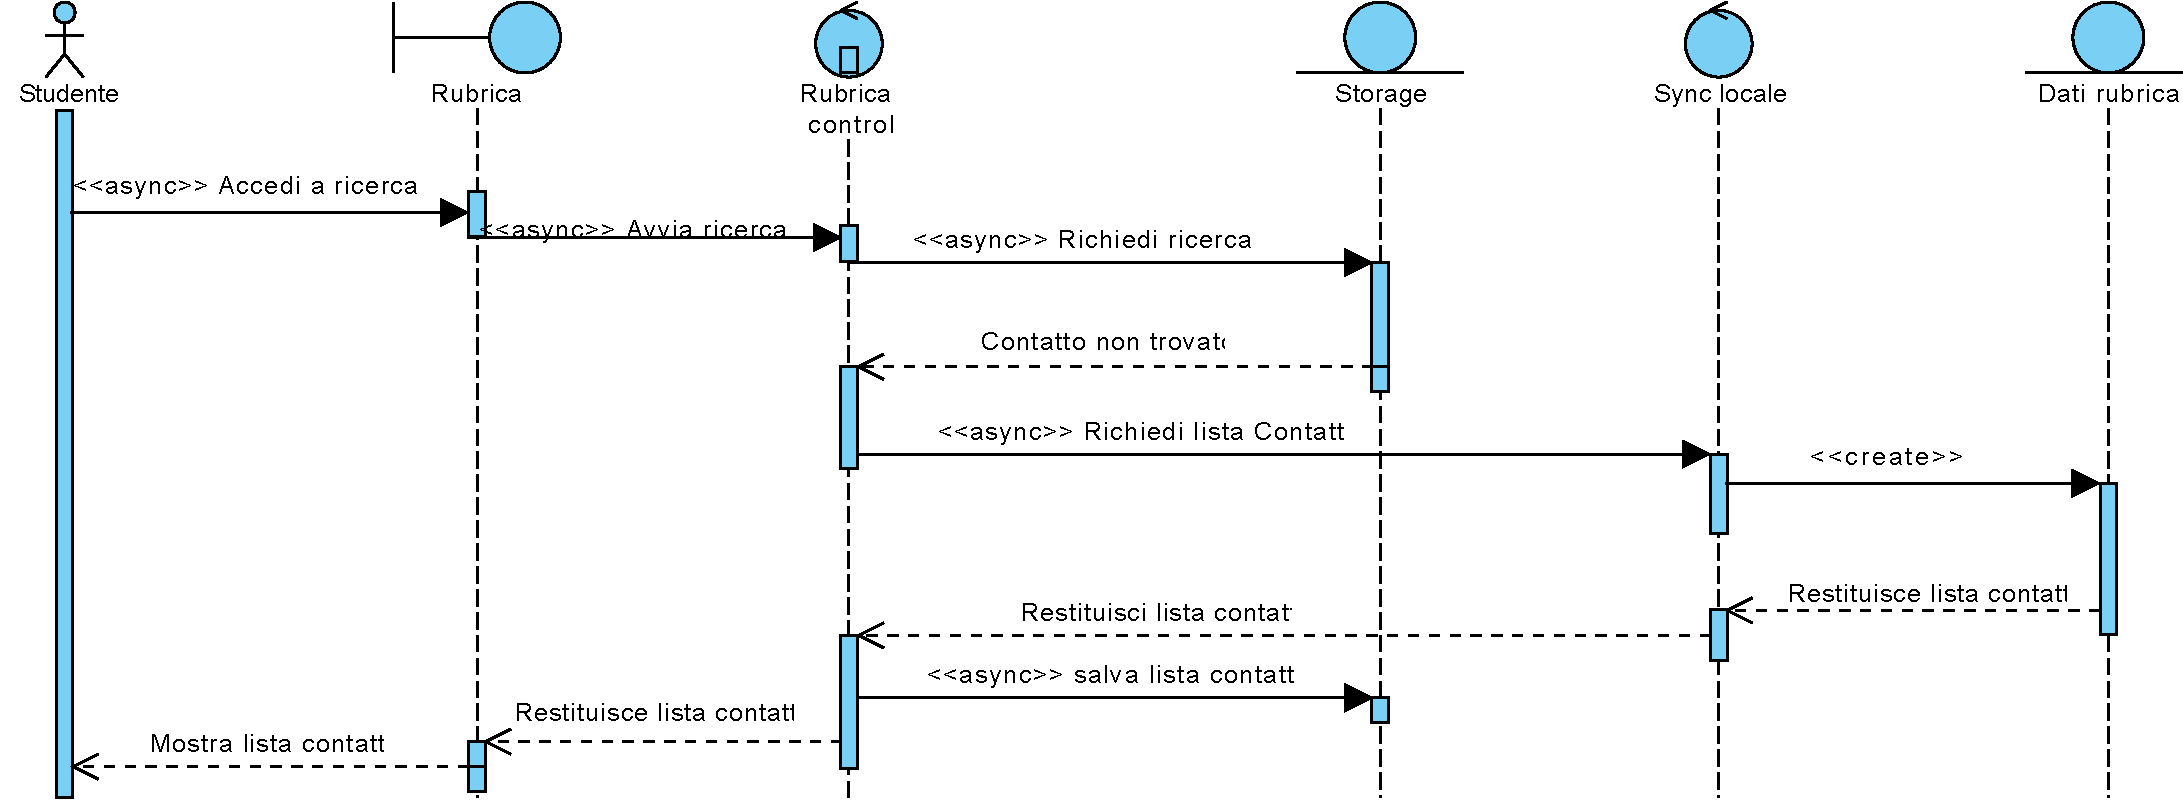
\includegraphics[height=3in,width=5in]{imgs/gruppo5/sequence1.pdf}
	\caption{Rubrica - Ricerca non filtarta}
	\label{fig:prova}
\end{figure}

\begin{figure}
	\centering
	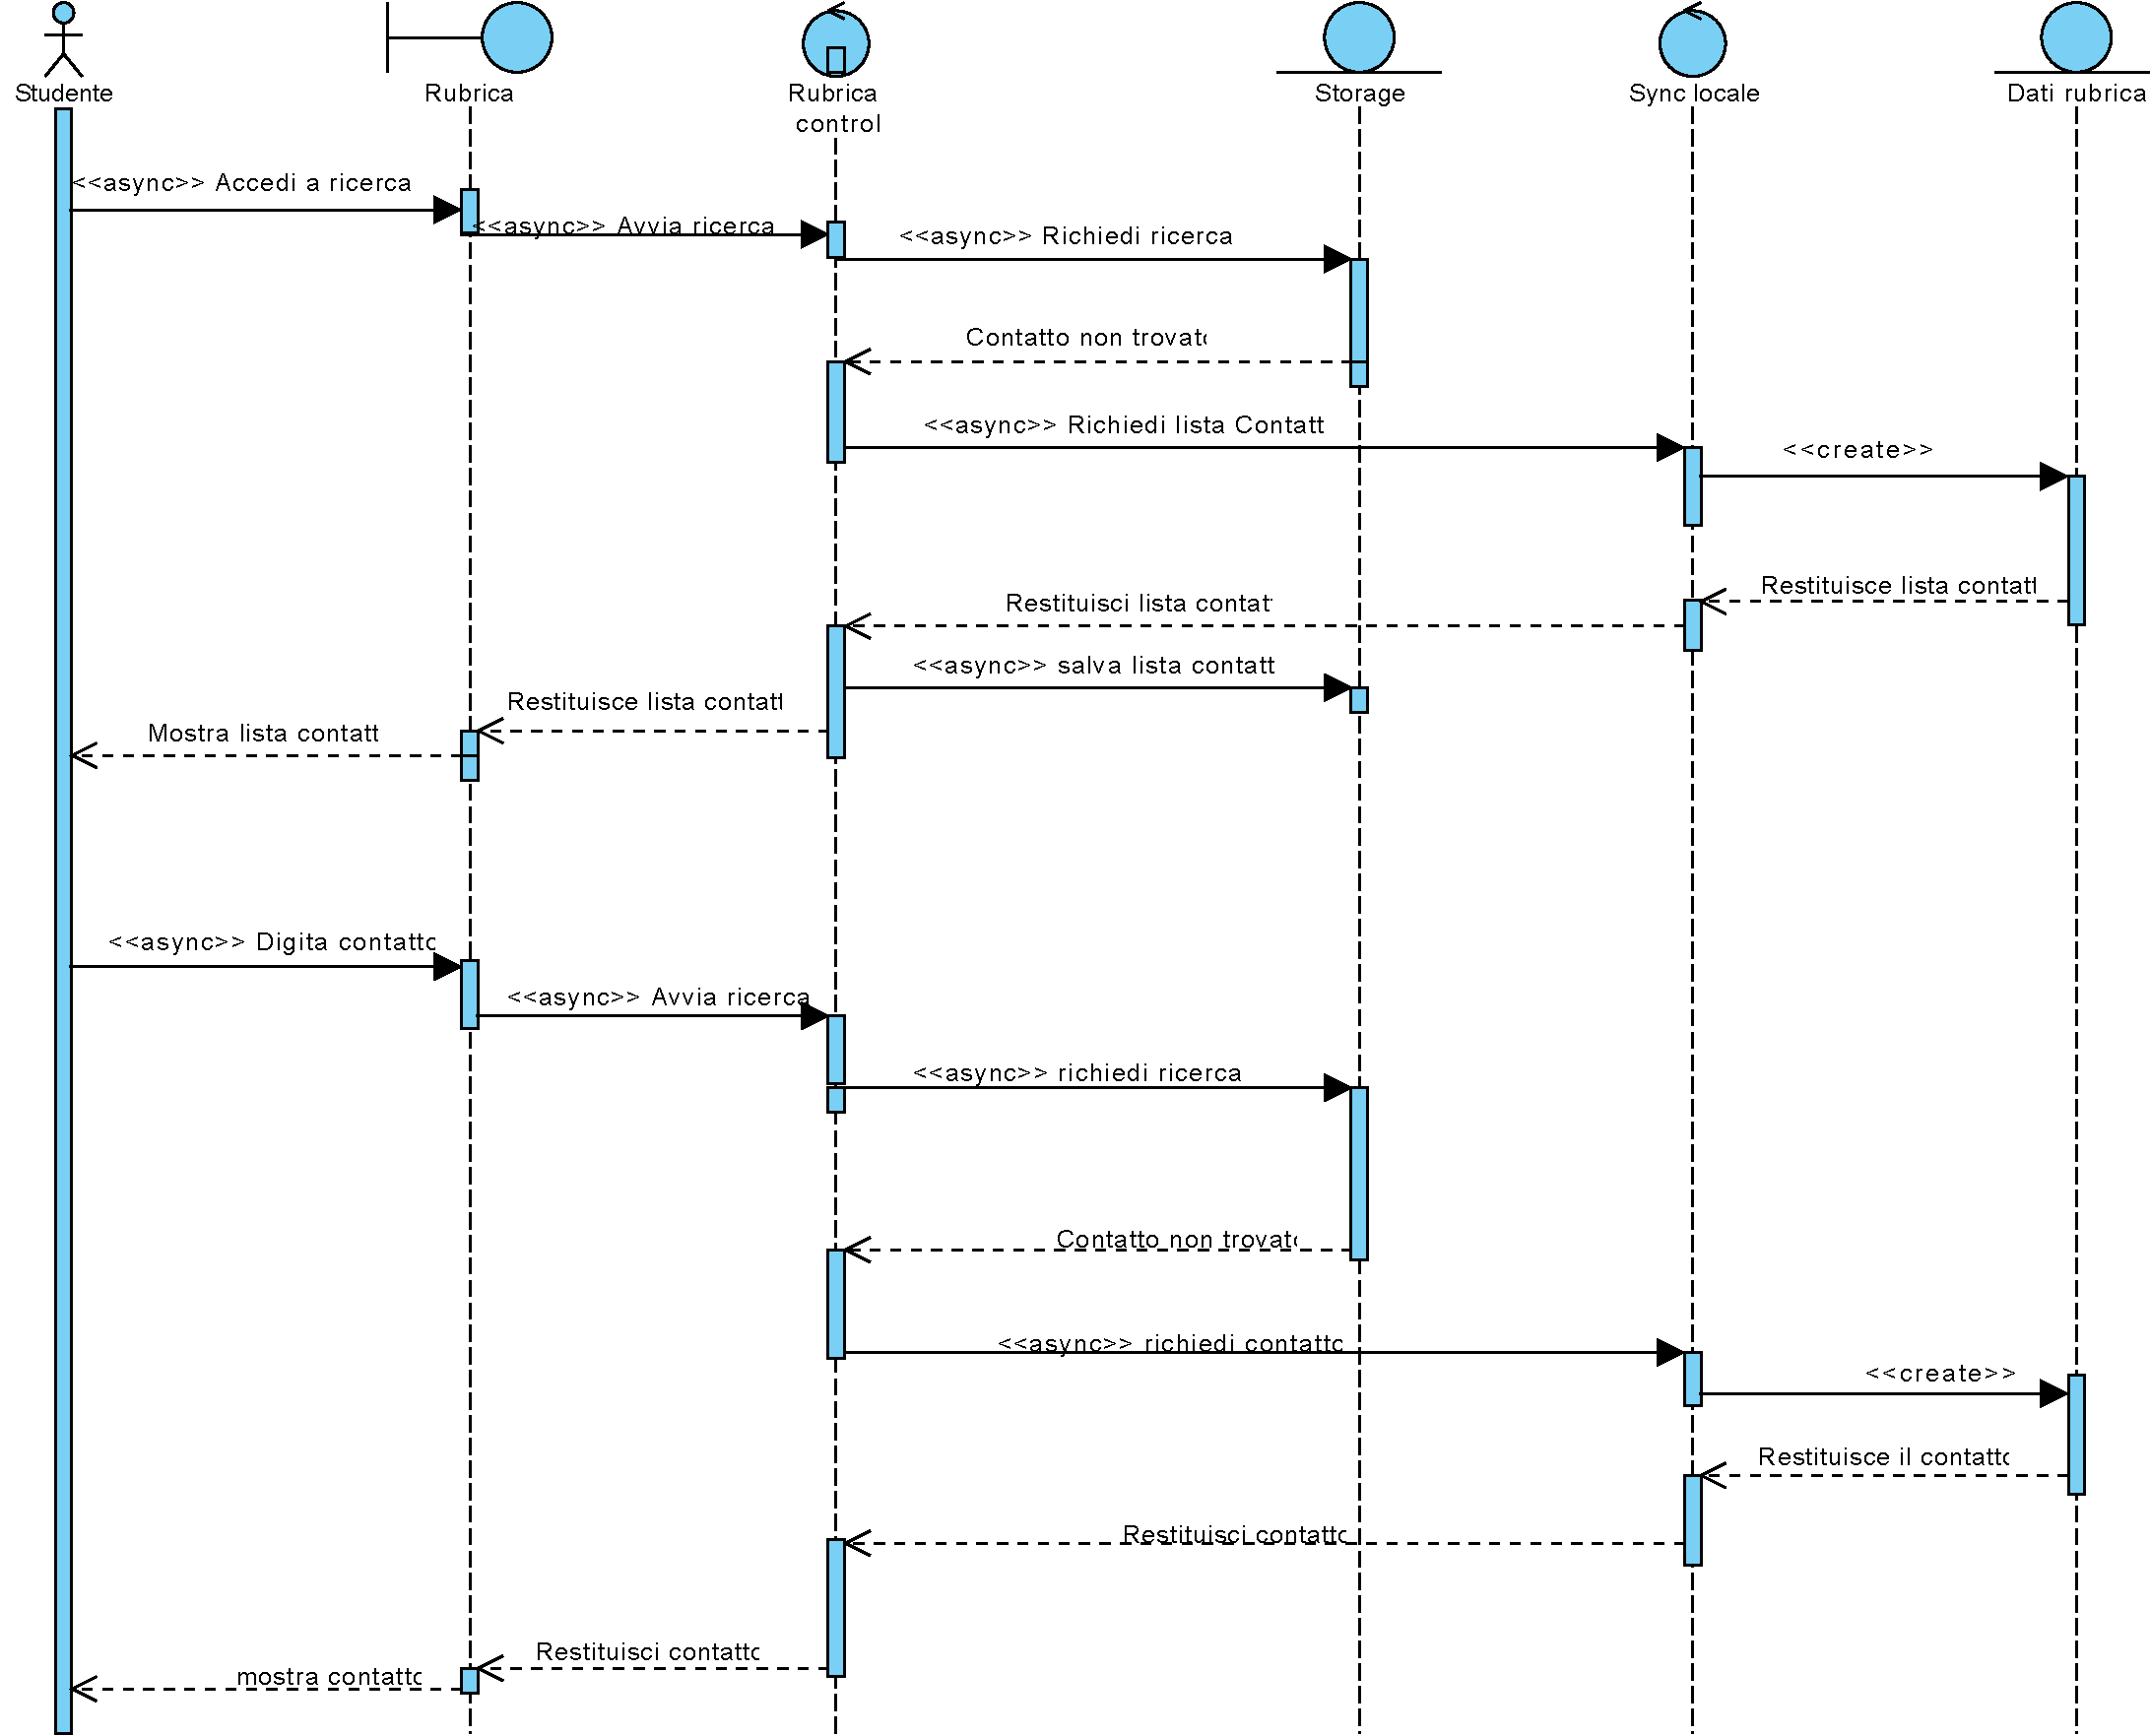
\includegraphics[height=3in,width=5in]{imgs/gruppo5/sequence2.pdf}
	\caption{Rubrica - Ricerca filtarta}
	\label{fig:prova}
\end{figure}

\begin{figure}
	\centering
	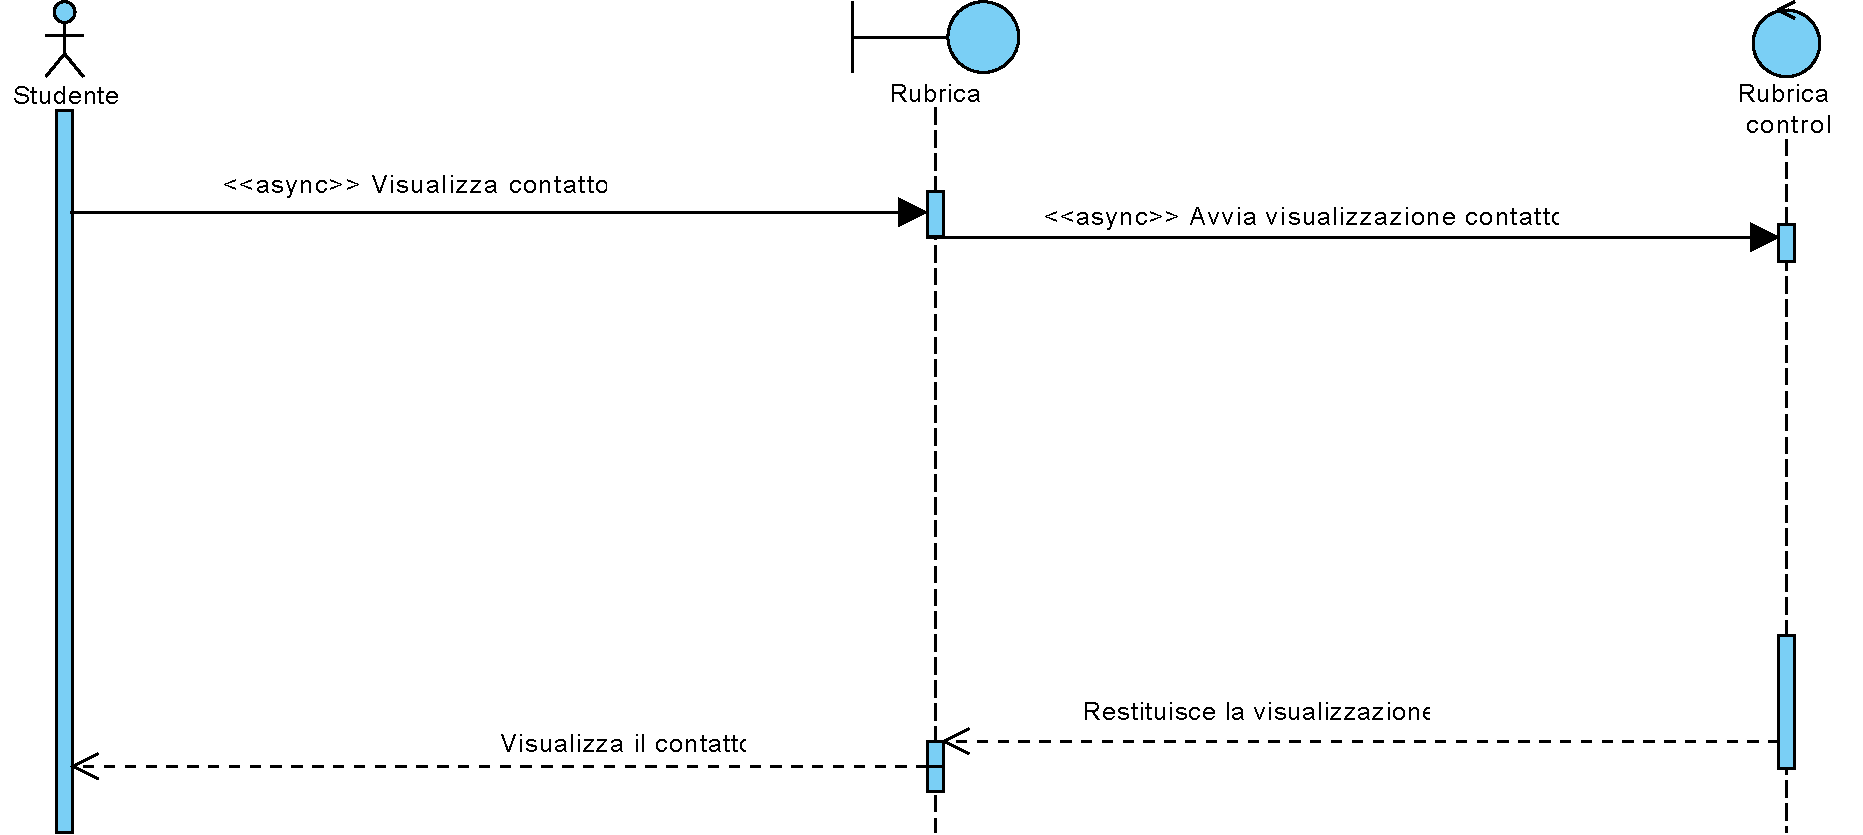
\includegraphics[height=3in,width=5in]{imgs/gruppo5/sequence3.pdf}
	\caption{Rubrica - Visualizza contatto}
	\label{fig:prova}
\end{figure}

\clearpage

\section{Diagramma delle attività}

\begin{figure}[!h]
	\centering
	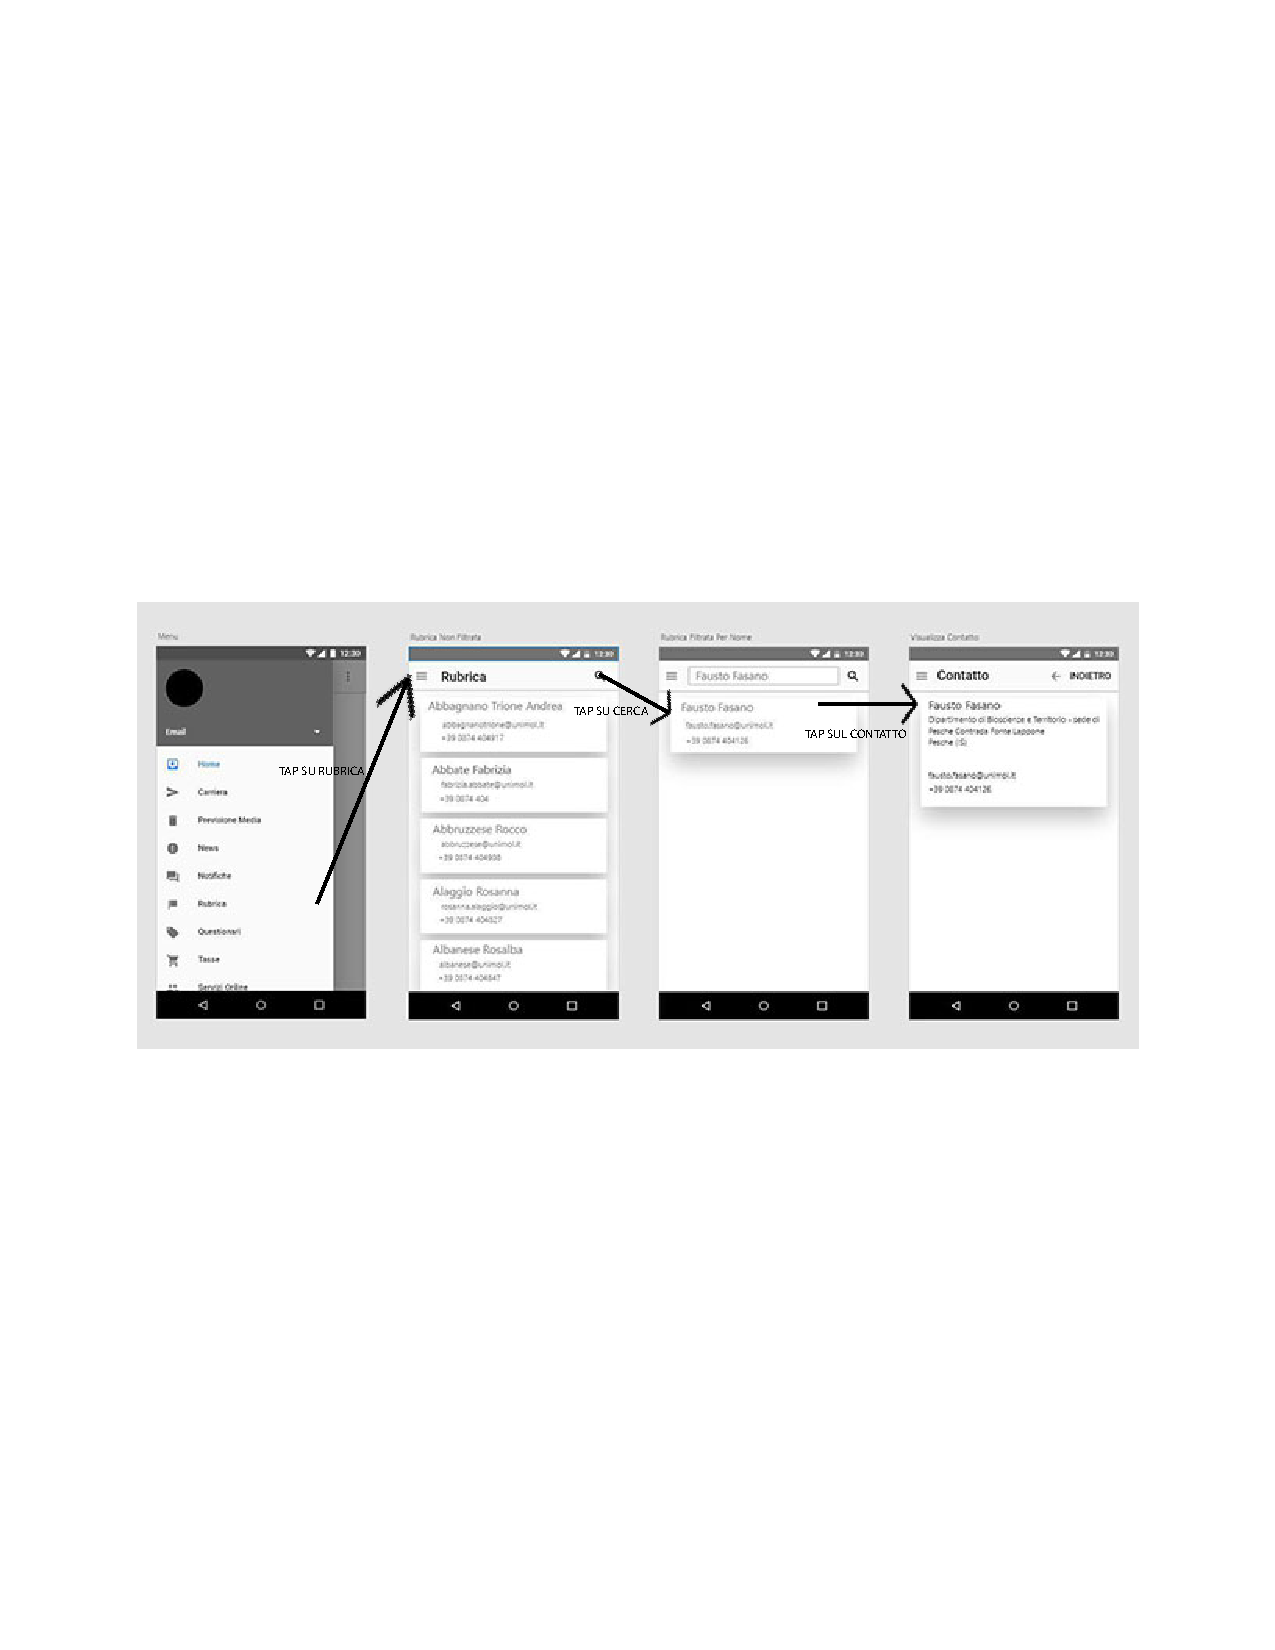
\includegraphics[height=8in,width=6in]{imgs/gruppo5/activity.pdf}
	\caption{Rubrica}
	\label{fig:prova}
\end{figure}

\clearpage
	%%%%%%%%%%%%%%%%%%%%%%%%%%%%%%%%%%%%%%%%%%%%%%%%%%%%%%%%%%%

\chapter{Modello del sistema - gruppo 6}
\label{ref:modSistemaGruppo6}

%%% Il gruppo 6 scriverà il suo modello del sistema. Esso dovrà includere: attori, casi d'uso (descrizione e tabella), scenari, diagrammi dei casi d'uso, diagrammi di sequenza, diagramma delle attività, screen mockups della funzionalità %%%

\section{Attori}
Descrivere gli attori che partecipano ai seguenti caso d'uso.

%%%%%%%%%%%%%%%PER QUANTO RIGUARDA IL NOSTRO ATTORE STUDENTE, VERRà INTEGRATO CON QUELLO DI TUTTI FACENDO UNA REF AD UNA LABEL
%N.B.:
%Per quanto riguarda la funzionalità chat \ref{nome-label} l'attore %studente ha in aggiunta le seguenti caratteristiche: ...

\section{Scenari}
Inserire qui gli scenari che sono un'istanza dei casi d'uso: gli scenari danno dei valori al flusso degli eventi dei casi d'uso. Esempio di caso d'uso "visualizza libretto": l'utente Antonio - che ha effettuato il login con username "Antonio" e password "antonioilmigliore" - accede alla sezione "libretto" e visualizza gli esami sostenuti Programmazione e Inglese con le votazioni rispettive di 25 e 30.

\section{Casi d'uso}
Per ogni caso d'uso inserire descrizione e tabella. Se il tuo caso d'uso prevede più attori di quelli che sono nella tabella sottostante di esempio, aggiungi una colonna nella sezione flusso degli eventi!

\paragraph{Caso d'uso 1 (sostituire con nome caso d'uso) \\} 

%%%%%%%%%%%%%% METTERE LABEL AI NOSTRI CASI D'USO
%\label{nome-label}

Lorem ipsum dolor sit amet... (sostituire con descrizione caso d'uso)

\begin{table}
%\normalsize % Dimensione testo normale
\small % Dimensione testo piccola
%\footnotesize % Dimensione testo piccolissima
%\scriptsize % Dimensione del testo ulteriormente più piccola
%\caption{} % Didascalia tabella
%\label{} % Etichetta per riferimenti incrociati
\begin{tabular}{| p{\useCaseLeft} | p{\useCaseNum} | p{\useCaseTwoCol} | p{\useCaseTwoCol} |}
	\hline
	\textbf{Nome caso d'uso} & \multicolumn{3}{p{\useCaseMulticol} |}{\textbf{Login}} \\
	\hline
	\textbf{Attori partecipanti} & \multicolumn{3}{p{\useCaseMulticol} |}{Inizializzato da \textbf{Utente}.} \\
	\hline
	\textbf{Condizioni d'ingresso} & \multicolumn{3}{p{\useCaseMulticol} |}{L'utente ha cliccato sul bottone di login.} \\
	\hline
	\textbf{Flusso degli eventi} & \textbf{\#} & \textbf{Utente} & \textbf{Sistema} \\
	\hline
	\textbf{} & \textbf{1} & \textbf{} & Propone una schermata per l'inserimento dei dati necessari per il login, e-mail e password dell'utente \\
	\hline
	\textbf{} & \textbf{2} & Inserisce i dati e sottomette la richiesta & \textbf{} \\
	\hline
	\textbf{} & \textbf{3} & \textbf{} & Controlla che siano stati inseriti entrambi i campi e avvia le operazioni di visualizzazione \\
	\hline
	\textbf{Eccezioni} & \multicolumn{3}{p{\useCaseMulticol} |}{3.1 Uno o entrambi i campi sono vuoti.\newline 3.2 Le credenziali inserite non sono valide (una o entrambe).} \\
	\hline
	\textbf{Condizioni d'uscita} & \multicolumn{3}{p{\useCaseMulticol} |}{Il sistema completa la login e dà accesso all'app o, in caso contrario, visualizza un messaggio di errore se non sono stati inseriti tutti i dati obbligatori, se le credenziali non sono corrette o se si verifica un insuccesso dell'operazione.} \\
	\hline
\end{tabular}
\end{table}

\section{Diagramma dei casi d'uso}

Inserire immagine del diagramma. Le immagini vanno caricate nella cartella imgs, va inserito il path corrispondente (nomefile.estensione) dopo il tag includegraphics e va cambiata la descrizione dell'immagine (caption) con un'etichetta opportuna. Sostituire l'immagine file-comuni-ai-gruppi/useCaseEsempio.png con quella desiderata.

\begin{figure}
	\centering
	\includegraphics[height=3in]{imgs/file-comuni-ai-gruppi/useCaseEsempio.png}
	\caption{Inserire descrizione}
	\label{fig:prova}
\end{figure}

\section{Diagramma di sequenza}
Inserire immagine del diagramma. Le immagini vanno caricate nella cartella imgs, va inserito il path corrispondente (nomefile.estensione) dopo il tag includegraphics e va cambiata la descrizione dell'immagine (caption) con un'etichetta opportuna. Sostituire l'immagine file-comuni-ai-gruppi/useCaseEsempio.png con quella desiderata.

\begin{figure}
	\centering
	\includegraphics[height=3in,width=5in]{imgs/file-comuni-ai-gruppi/SequenceDgEsempio.png}
	\caption{Inserire descrizione}
	\label{fig:prova}
\end{figure}

\section{Diagramma delle attività}
%%% START activities chat studenti %%%
\begin{figure}
\subsection{Activities relative alla chat dell'App Studenti}
	\centering
	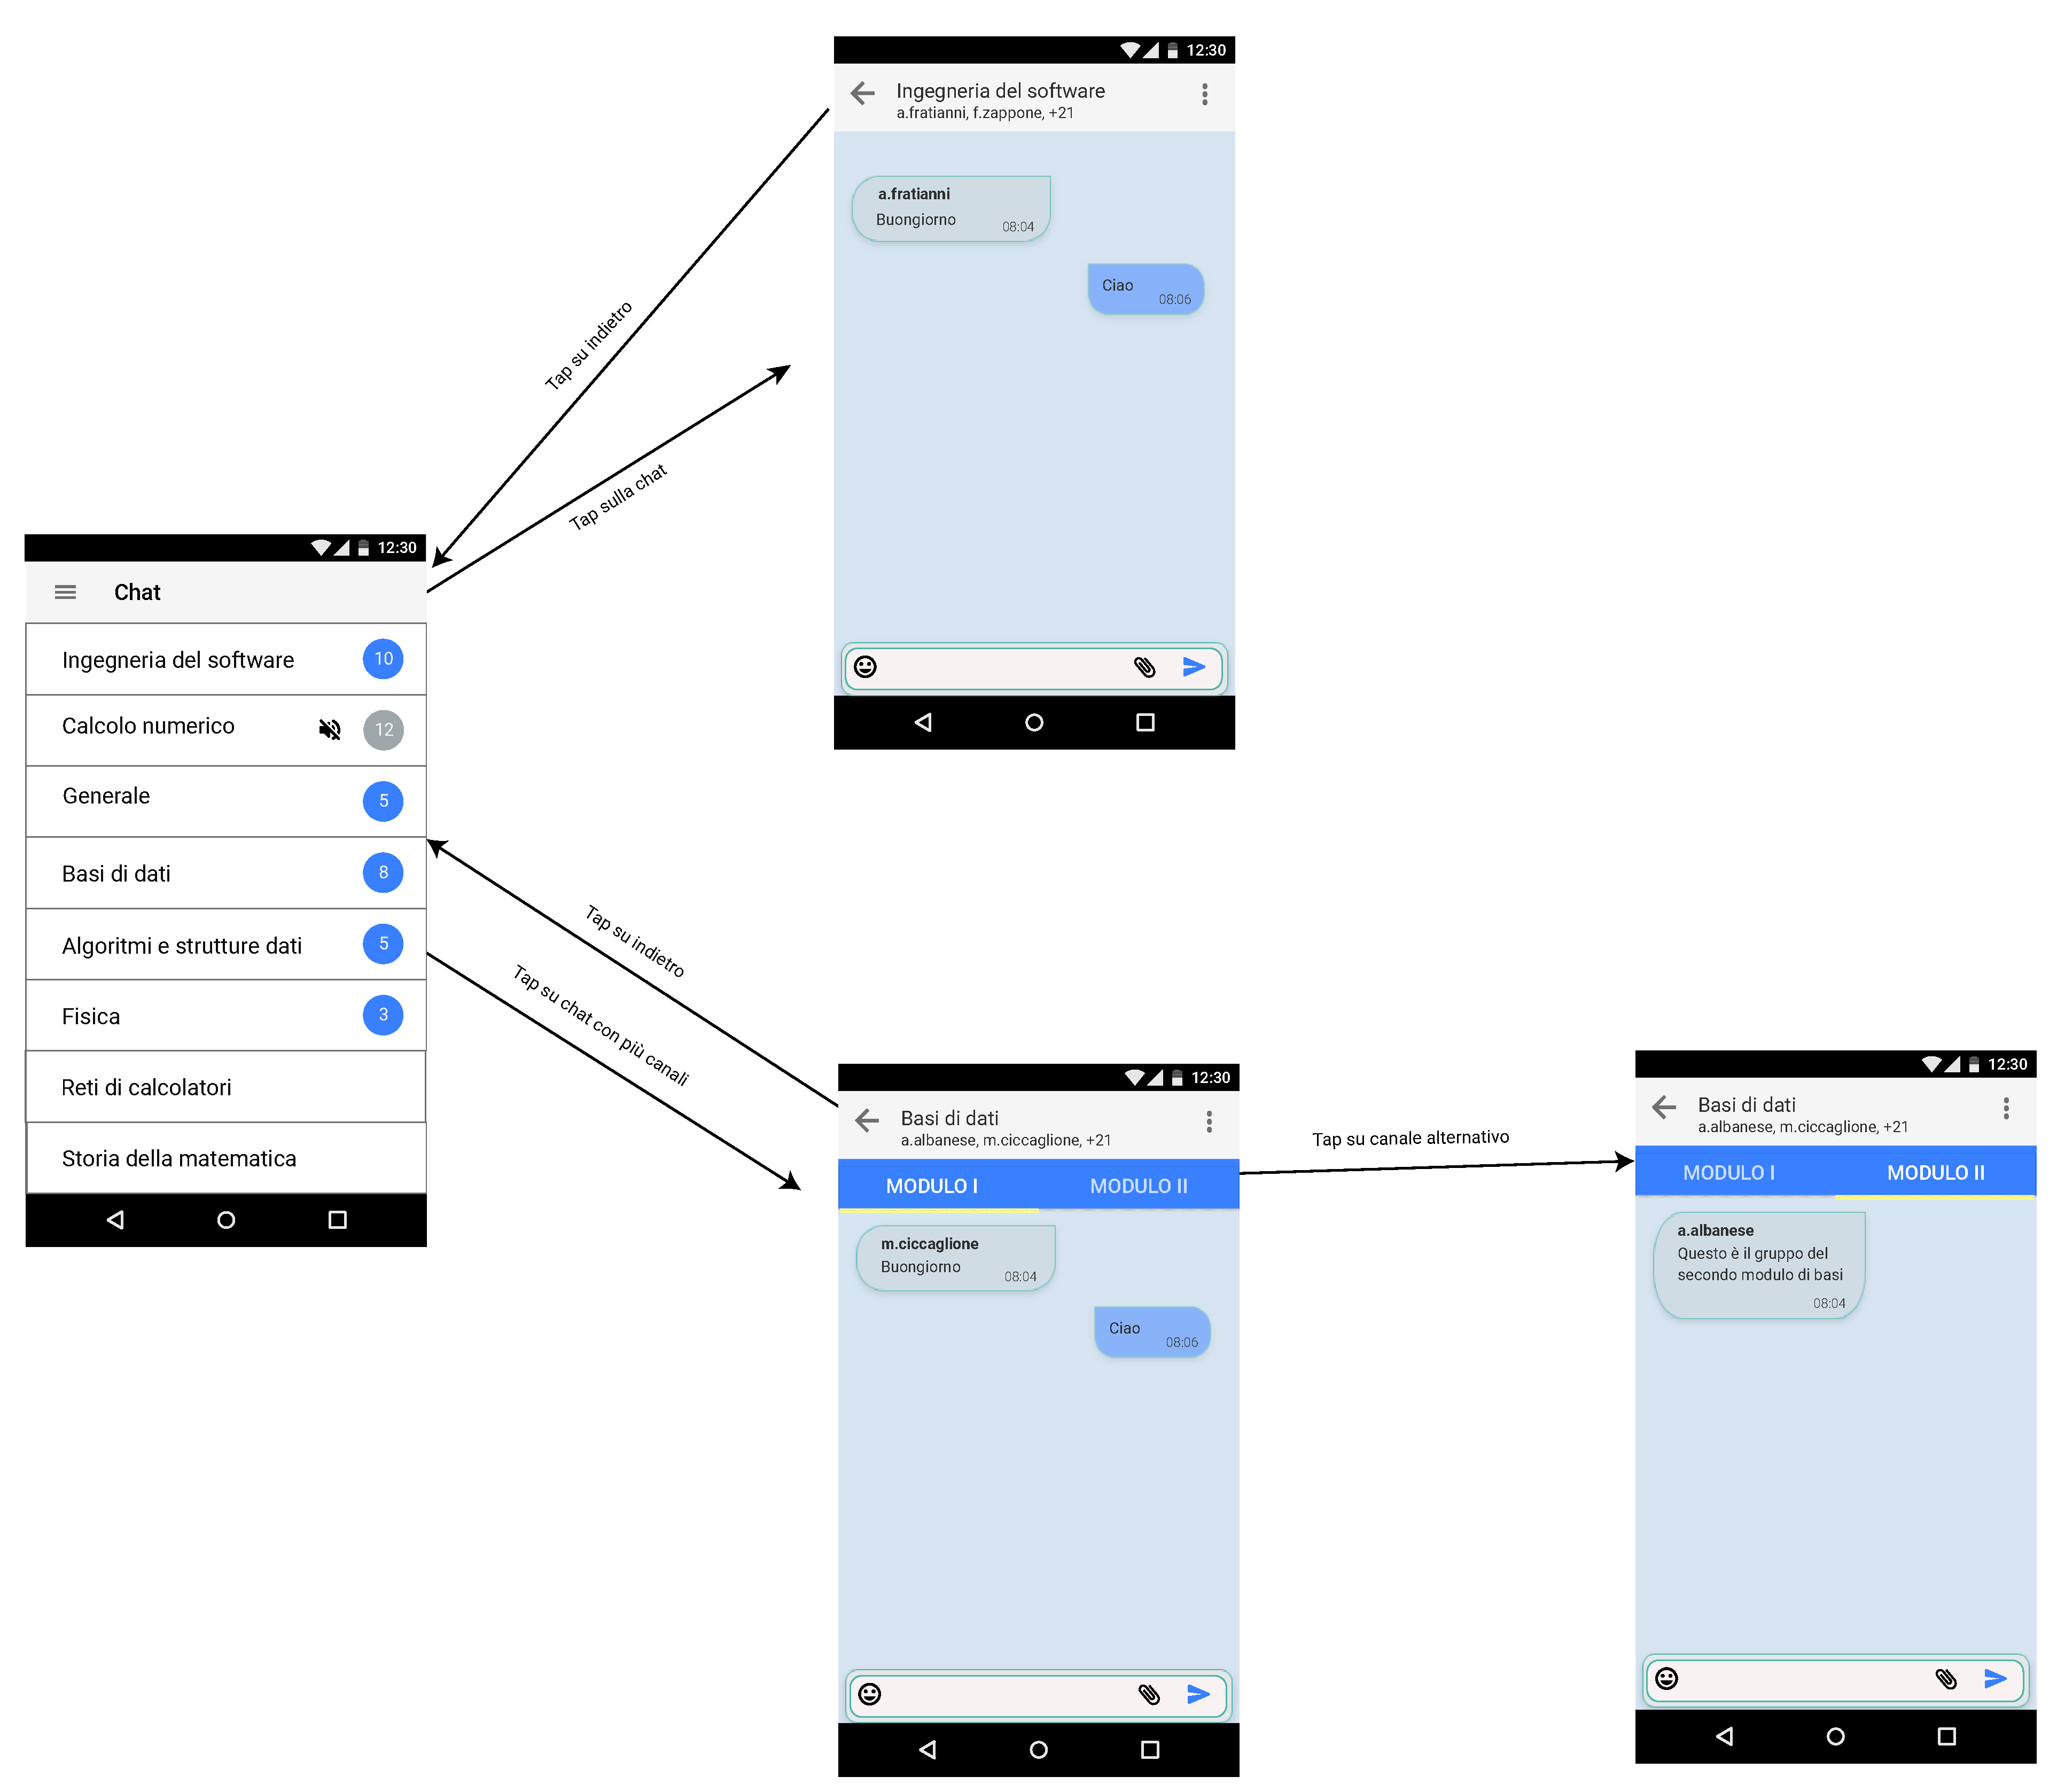
\includegraphics[width=0.9\textwidth]{imgs/gruppo6/activities/act_cus1_visualizza_canale.pdf}
	\caption{CUS 1 - Visualizza canale}
	\label{fig:cus1}
\end{figure}

\begin{figure}
	\centering
	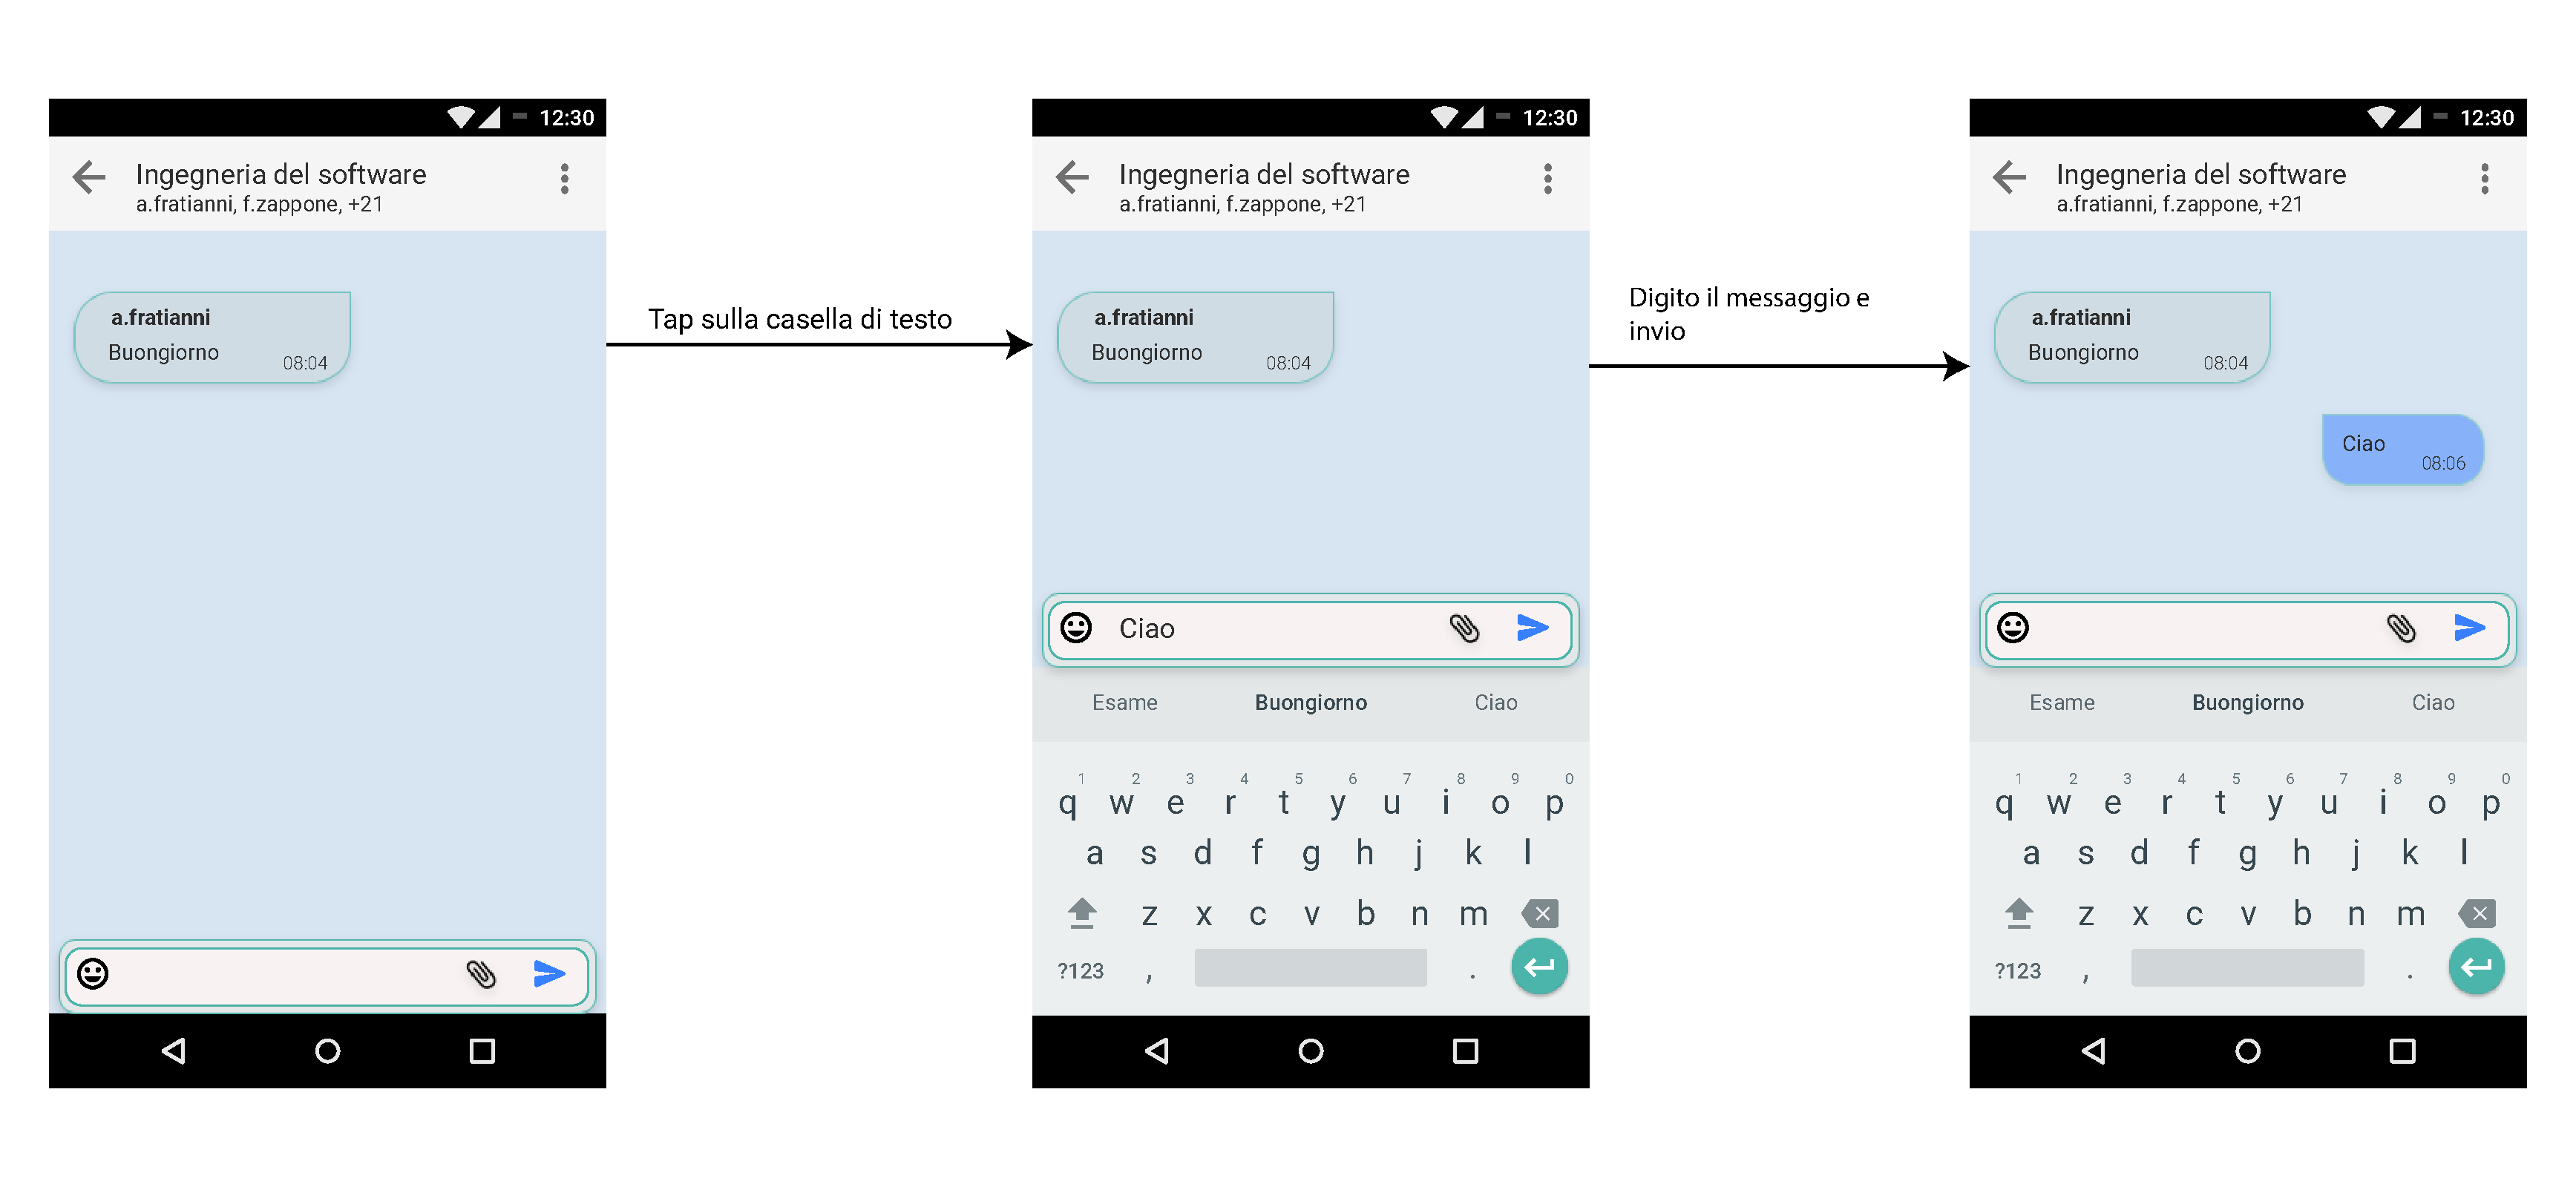
\includegraphics[width=0.9\textwidth]{imgs/gruppo6/activities/act_cus2_invio_messaggio.pdf}
	\caption{CUS2 - Invio messaggio}
	\label{fig:cus2}
\end{figure}

\begin{figure}
	\centering
	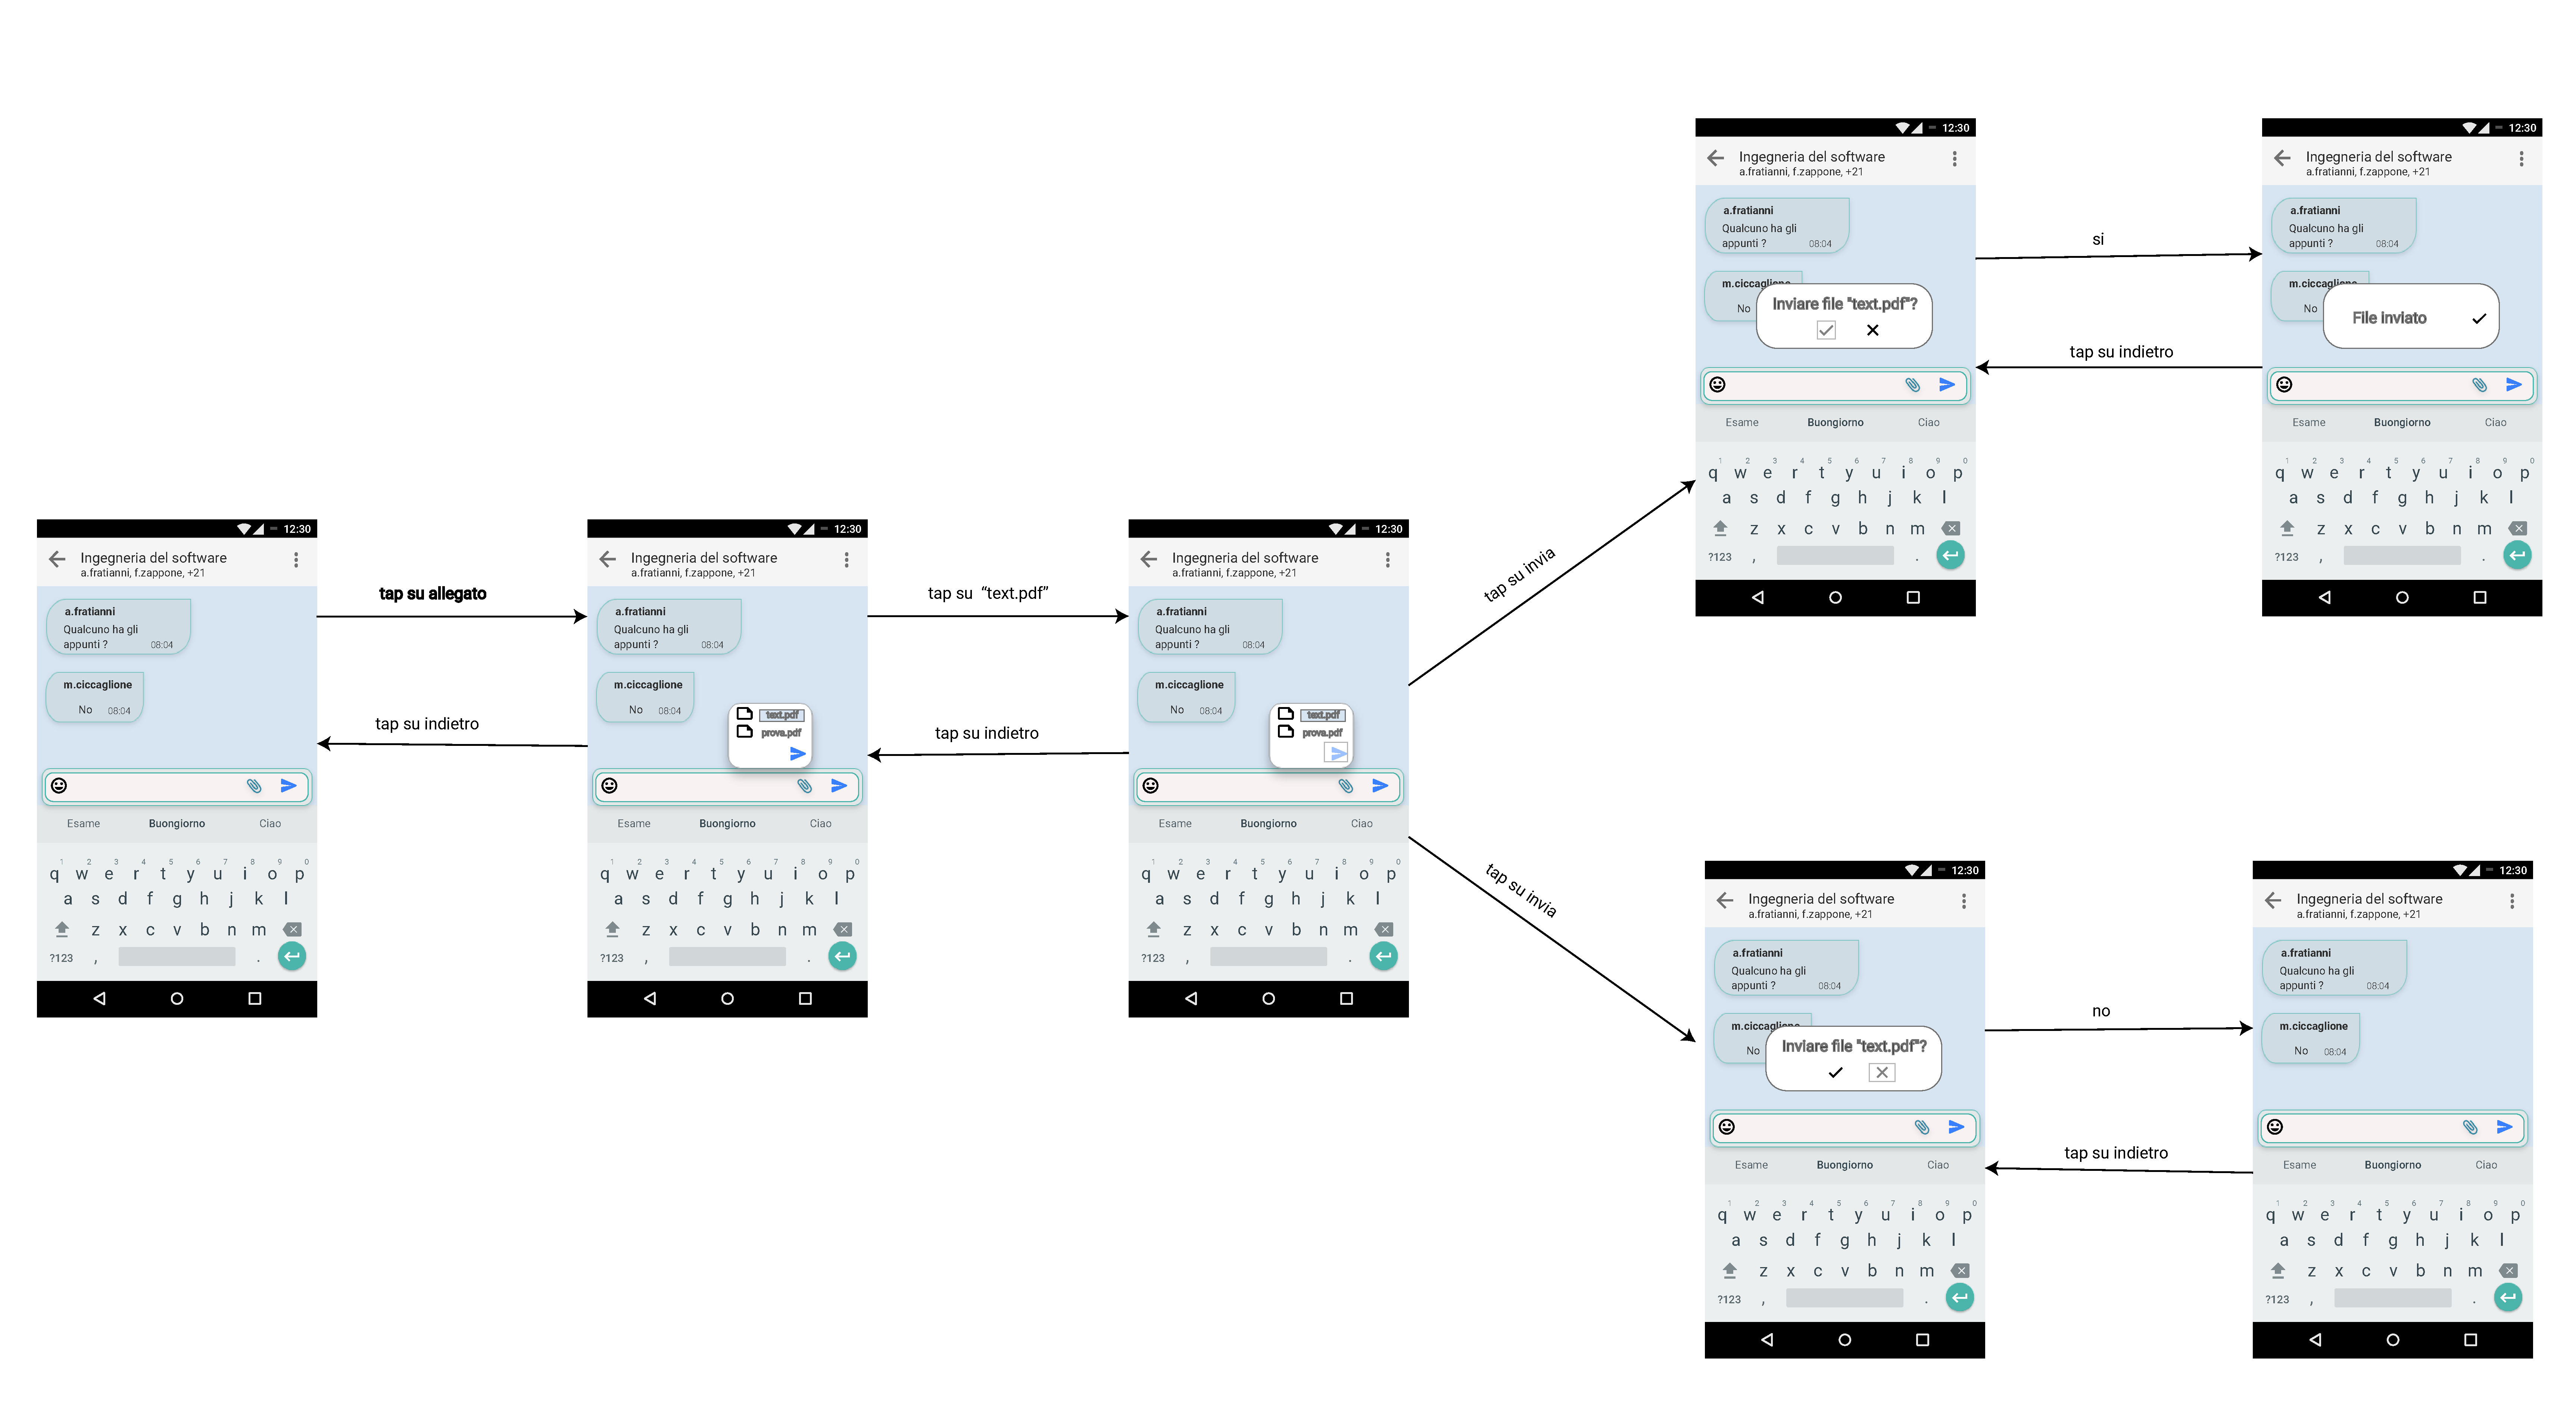
\includegraphics[width=0.9\textwidth]{imgs/gruppo6/activities/act_cus3_invia_allegato.pdf}
	\caption{CUS3 - Invio Allegato}
	\label{fig:cus3-1}
\end{figure}

\begin{figure}
	\centering
	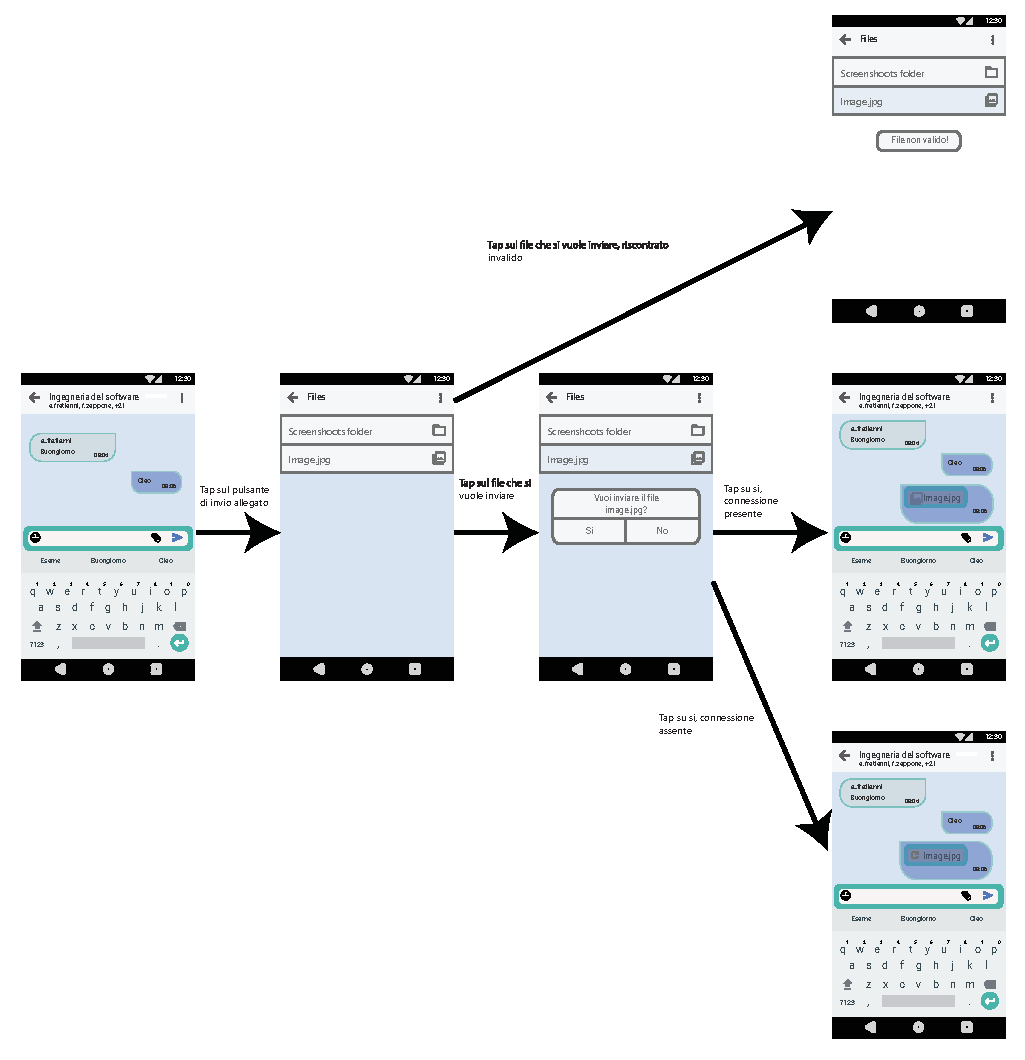
\includegraphics[width=0.9\textwidth]{imgs/gruppo6/activities/act_cus3_invio_allegato2.pdf}
	\caption{CUS3 - Invio Allegato (es. 2)}
	\label{fig:cus3-2}
\end{figure}

\begin{figure}
	\centering
	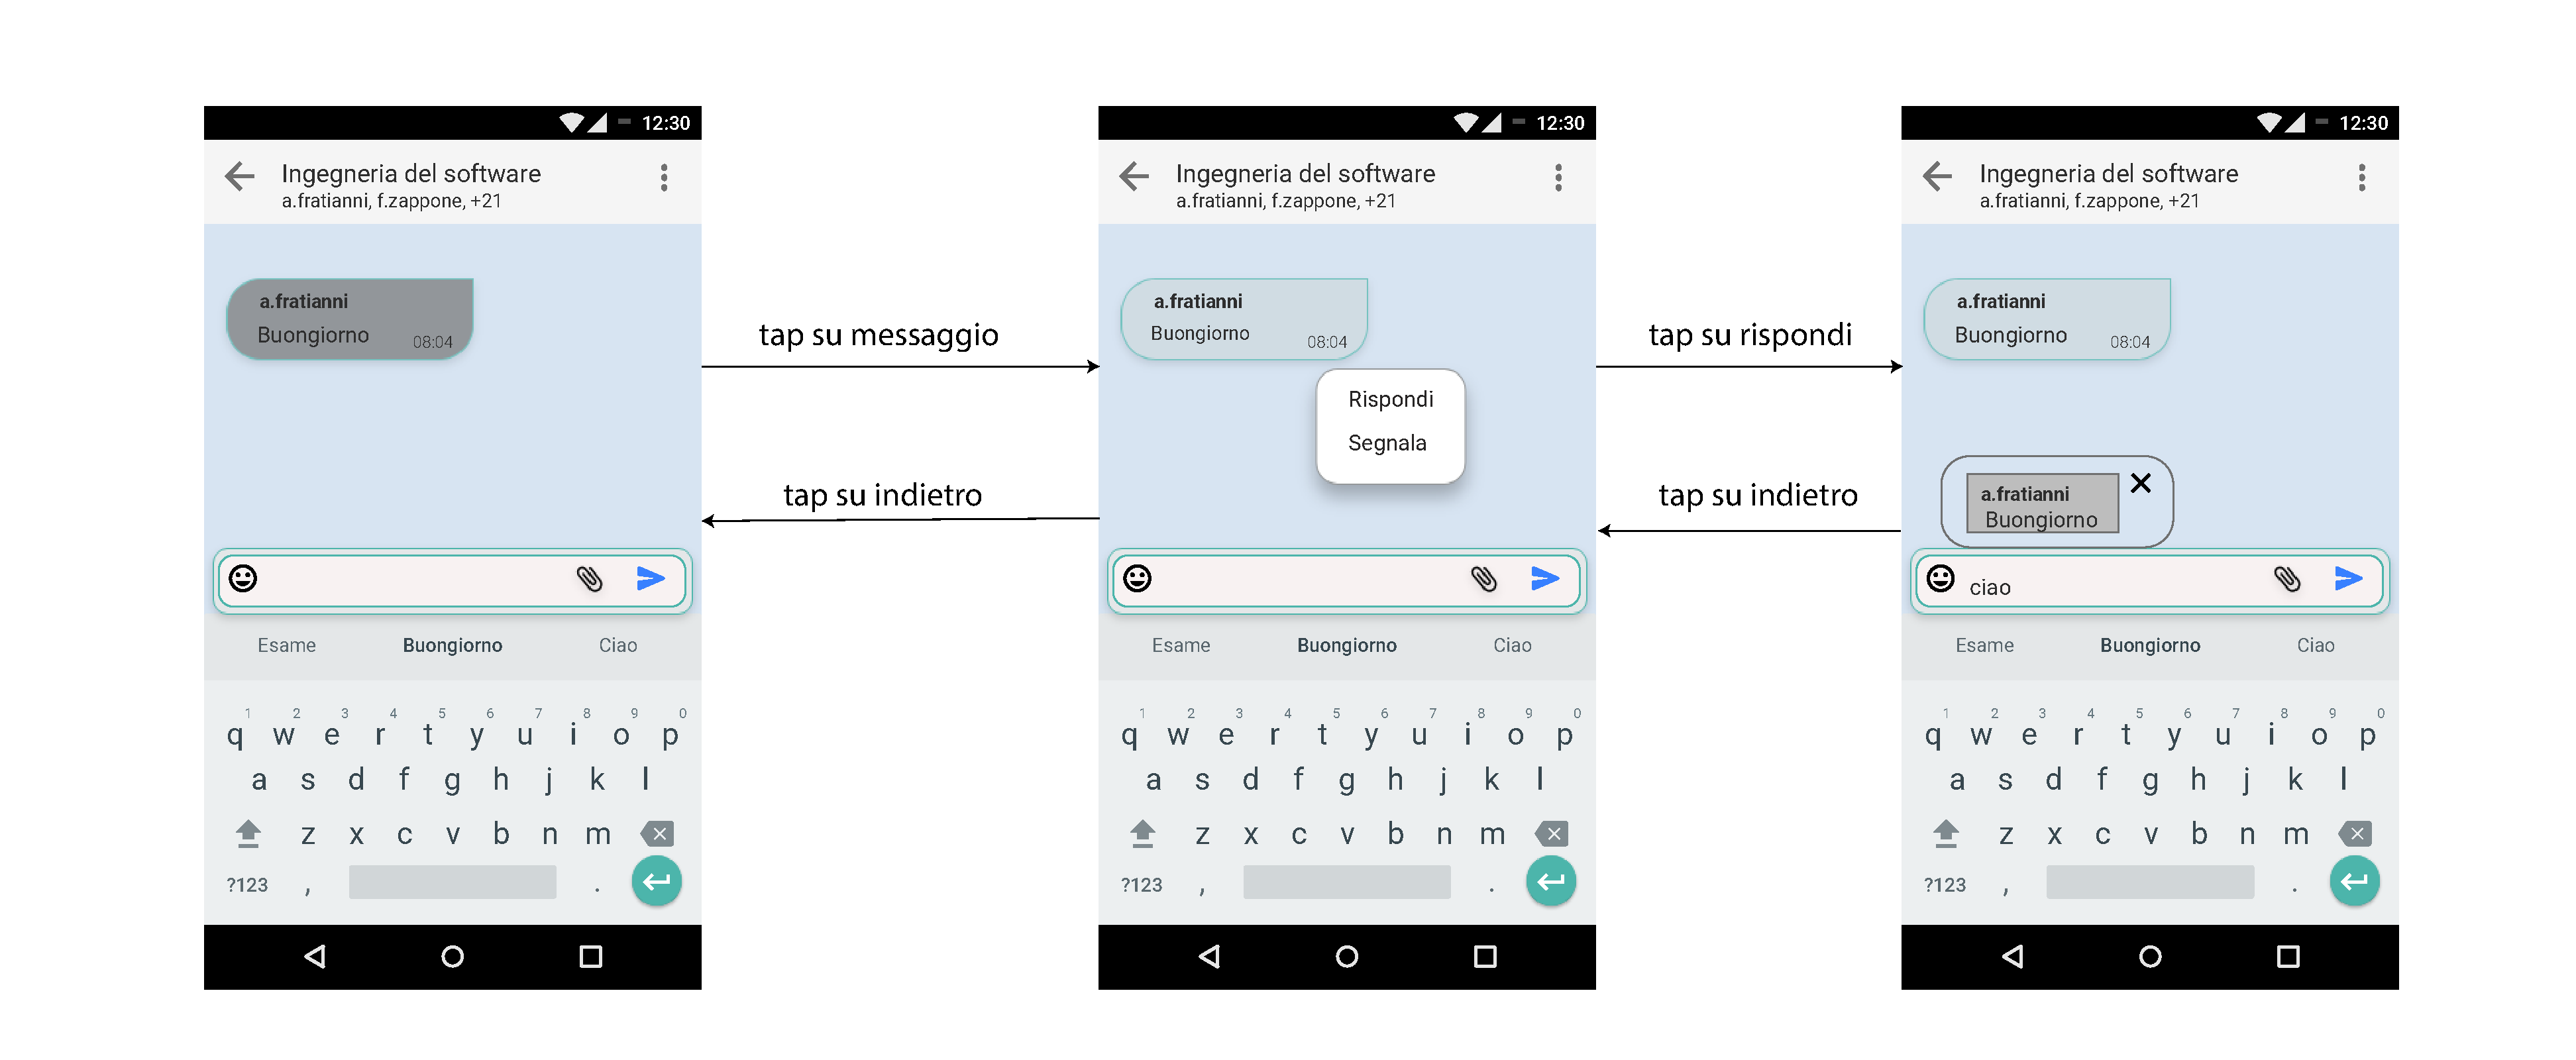
\includegraphics[width=0.9\textwidth]{imgs/gruppo6/activities/act_cus4_rispondi_singolo_messaggio.pdf}
	\caption{CUS4 - Rispondi al messaggio}
	\label{fig:cus4}
\end{figure}

\begin{figure}
	\centering
	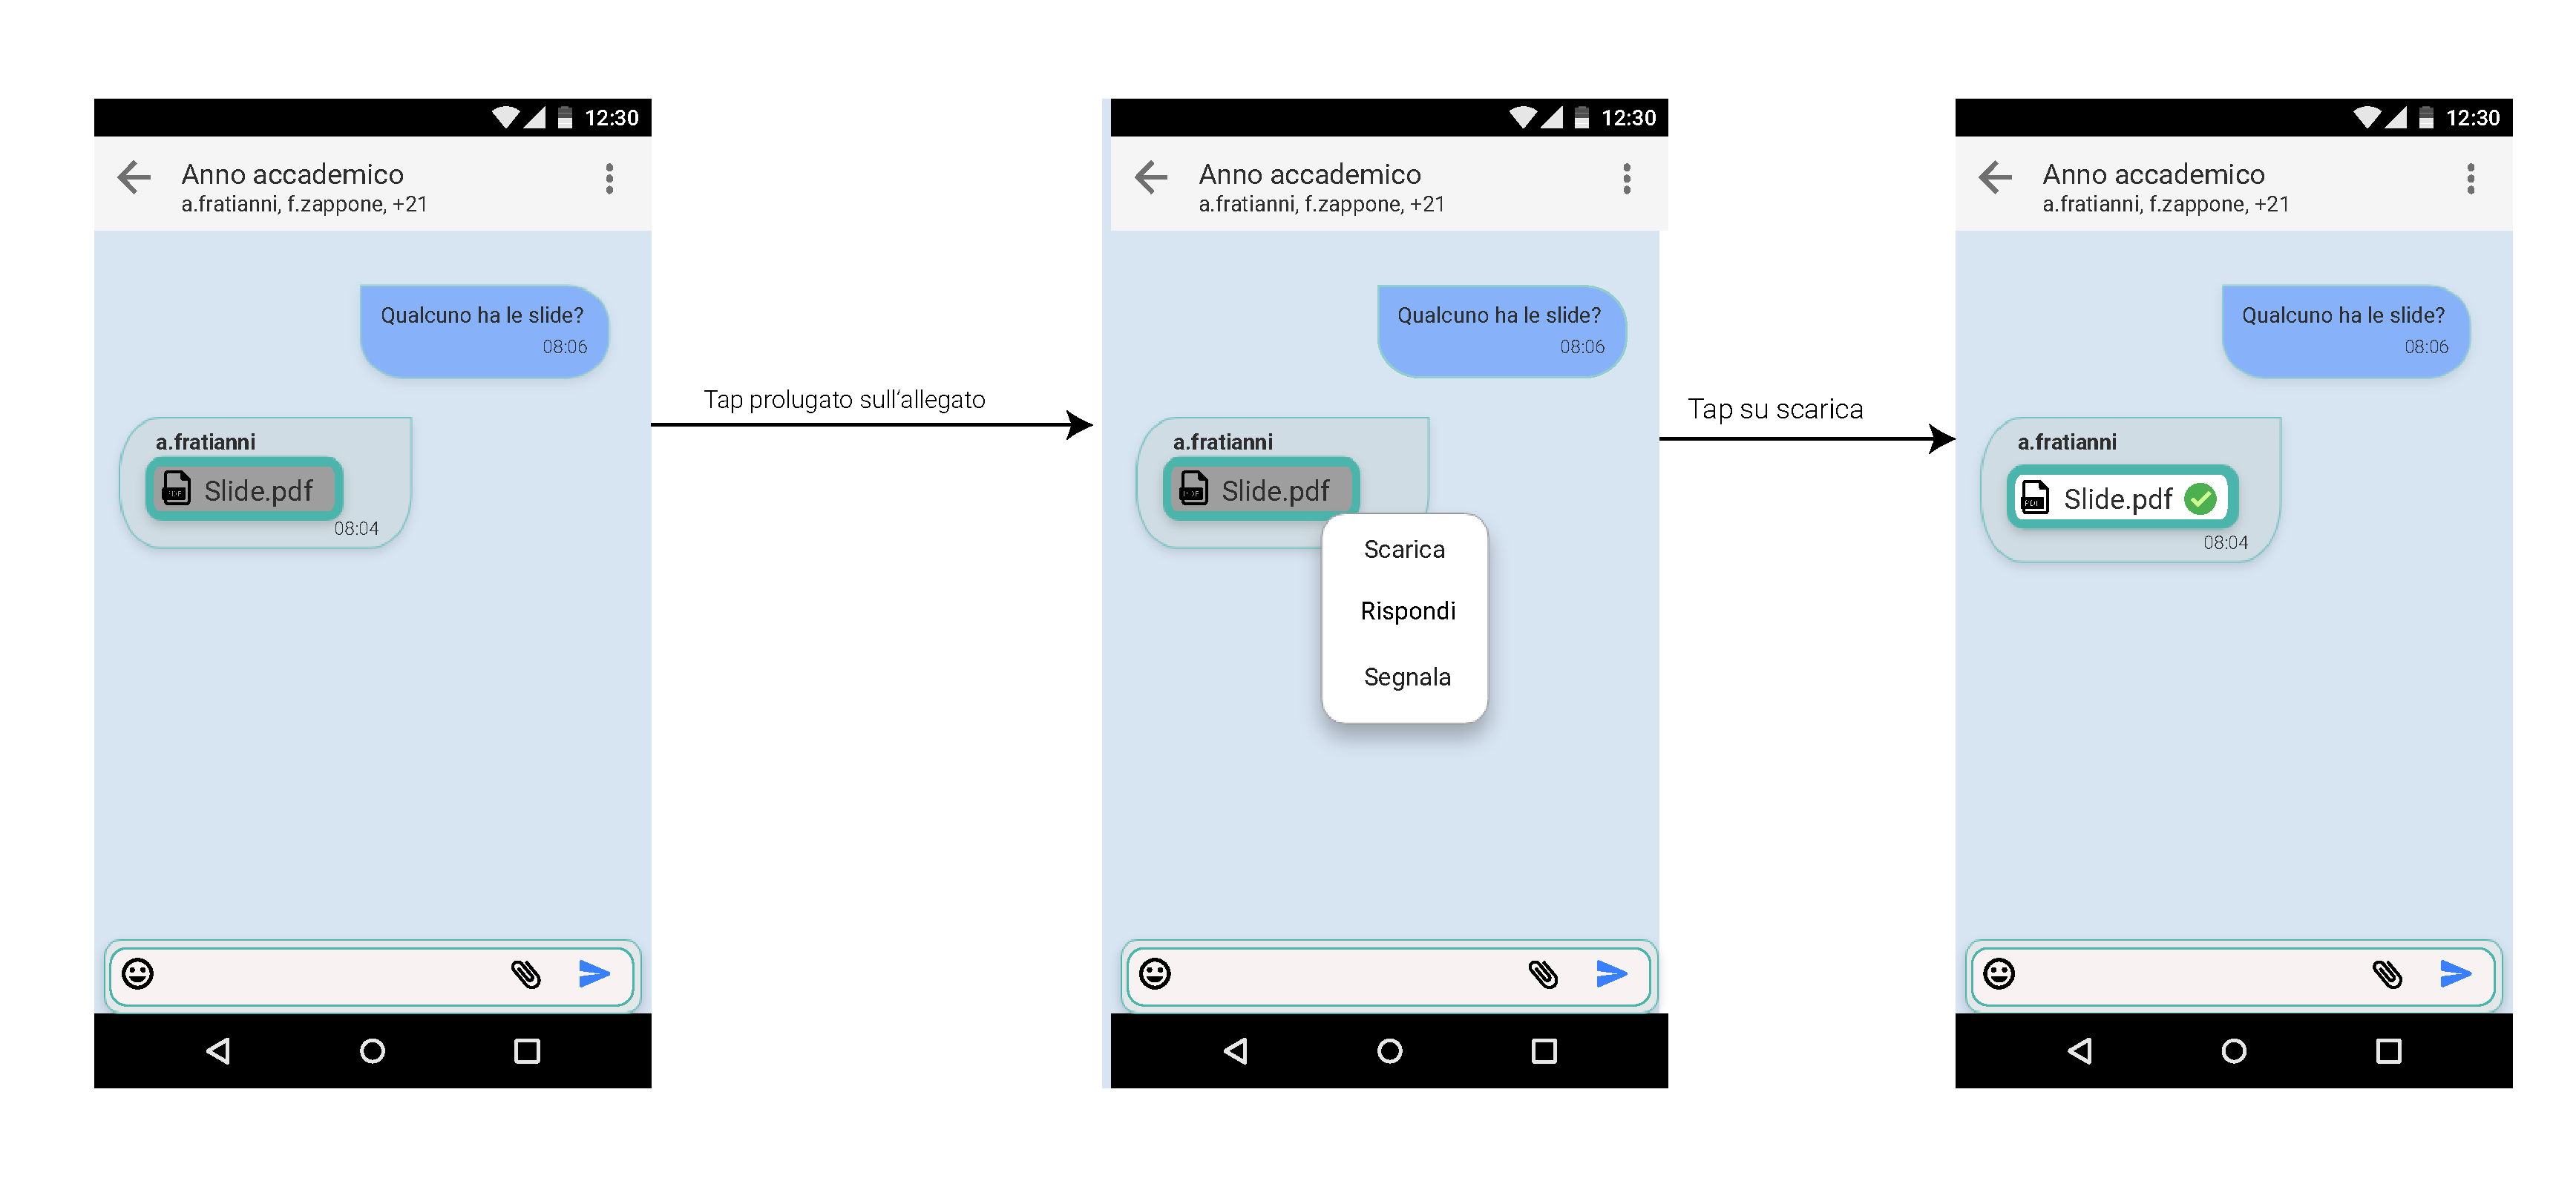
\includegraphics[width=0.9\textwidth]{imgs/gruppo6/activities/act_cus5_scarica_allegato.pdf}
	\caption{CUS5 - Scarica allegato}
	\label{fig:cus5}
\end{figure}

\begin{figure}
	\centering
	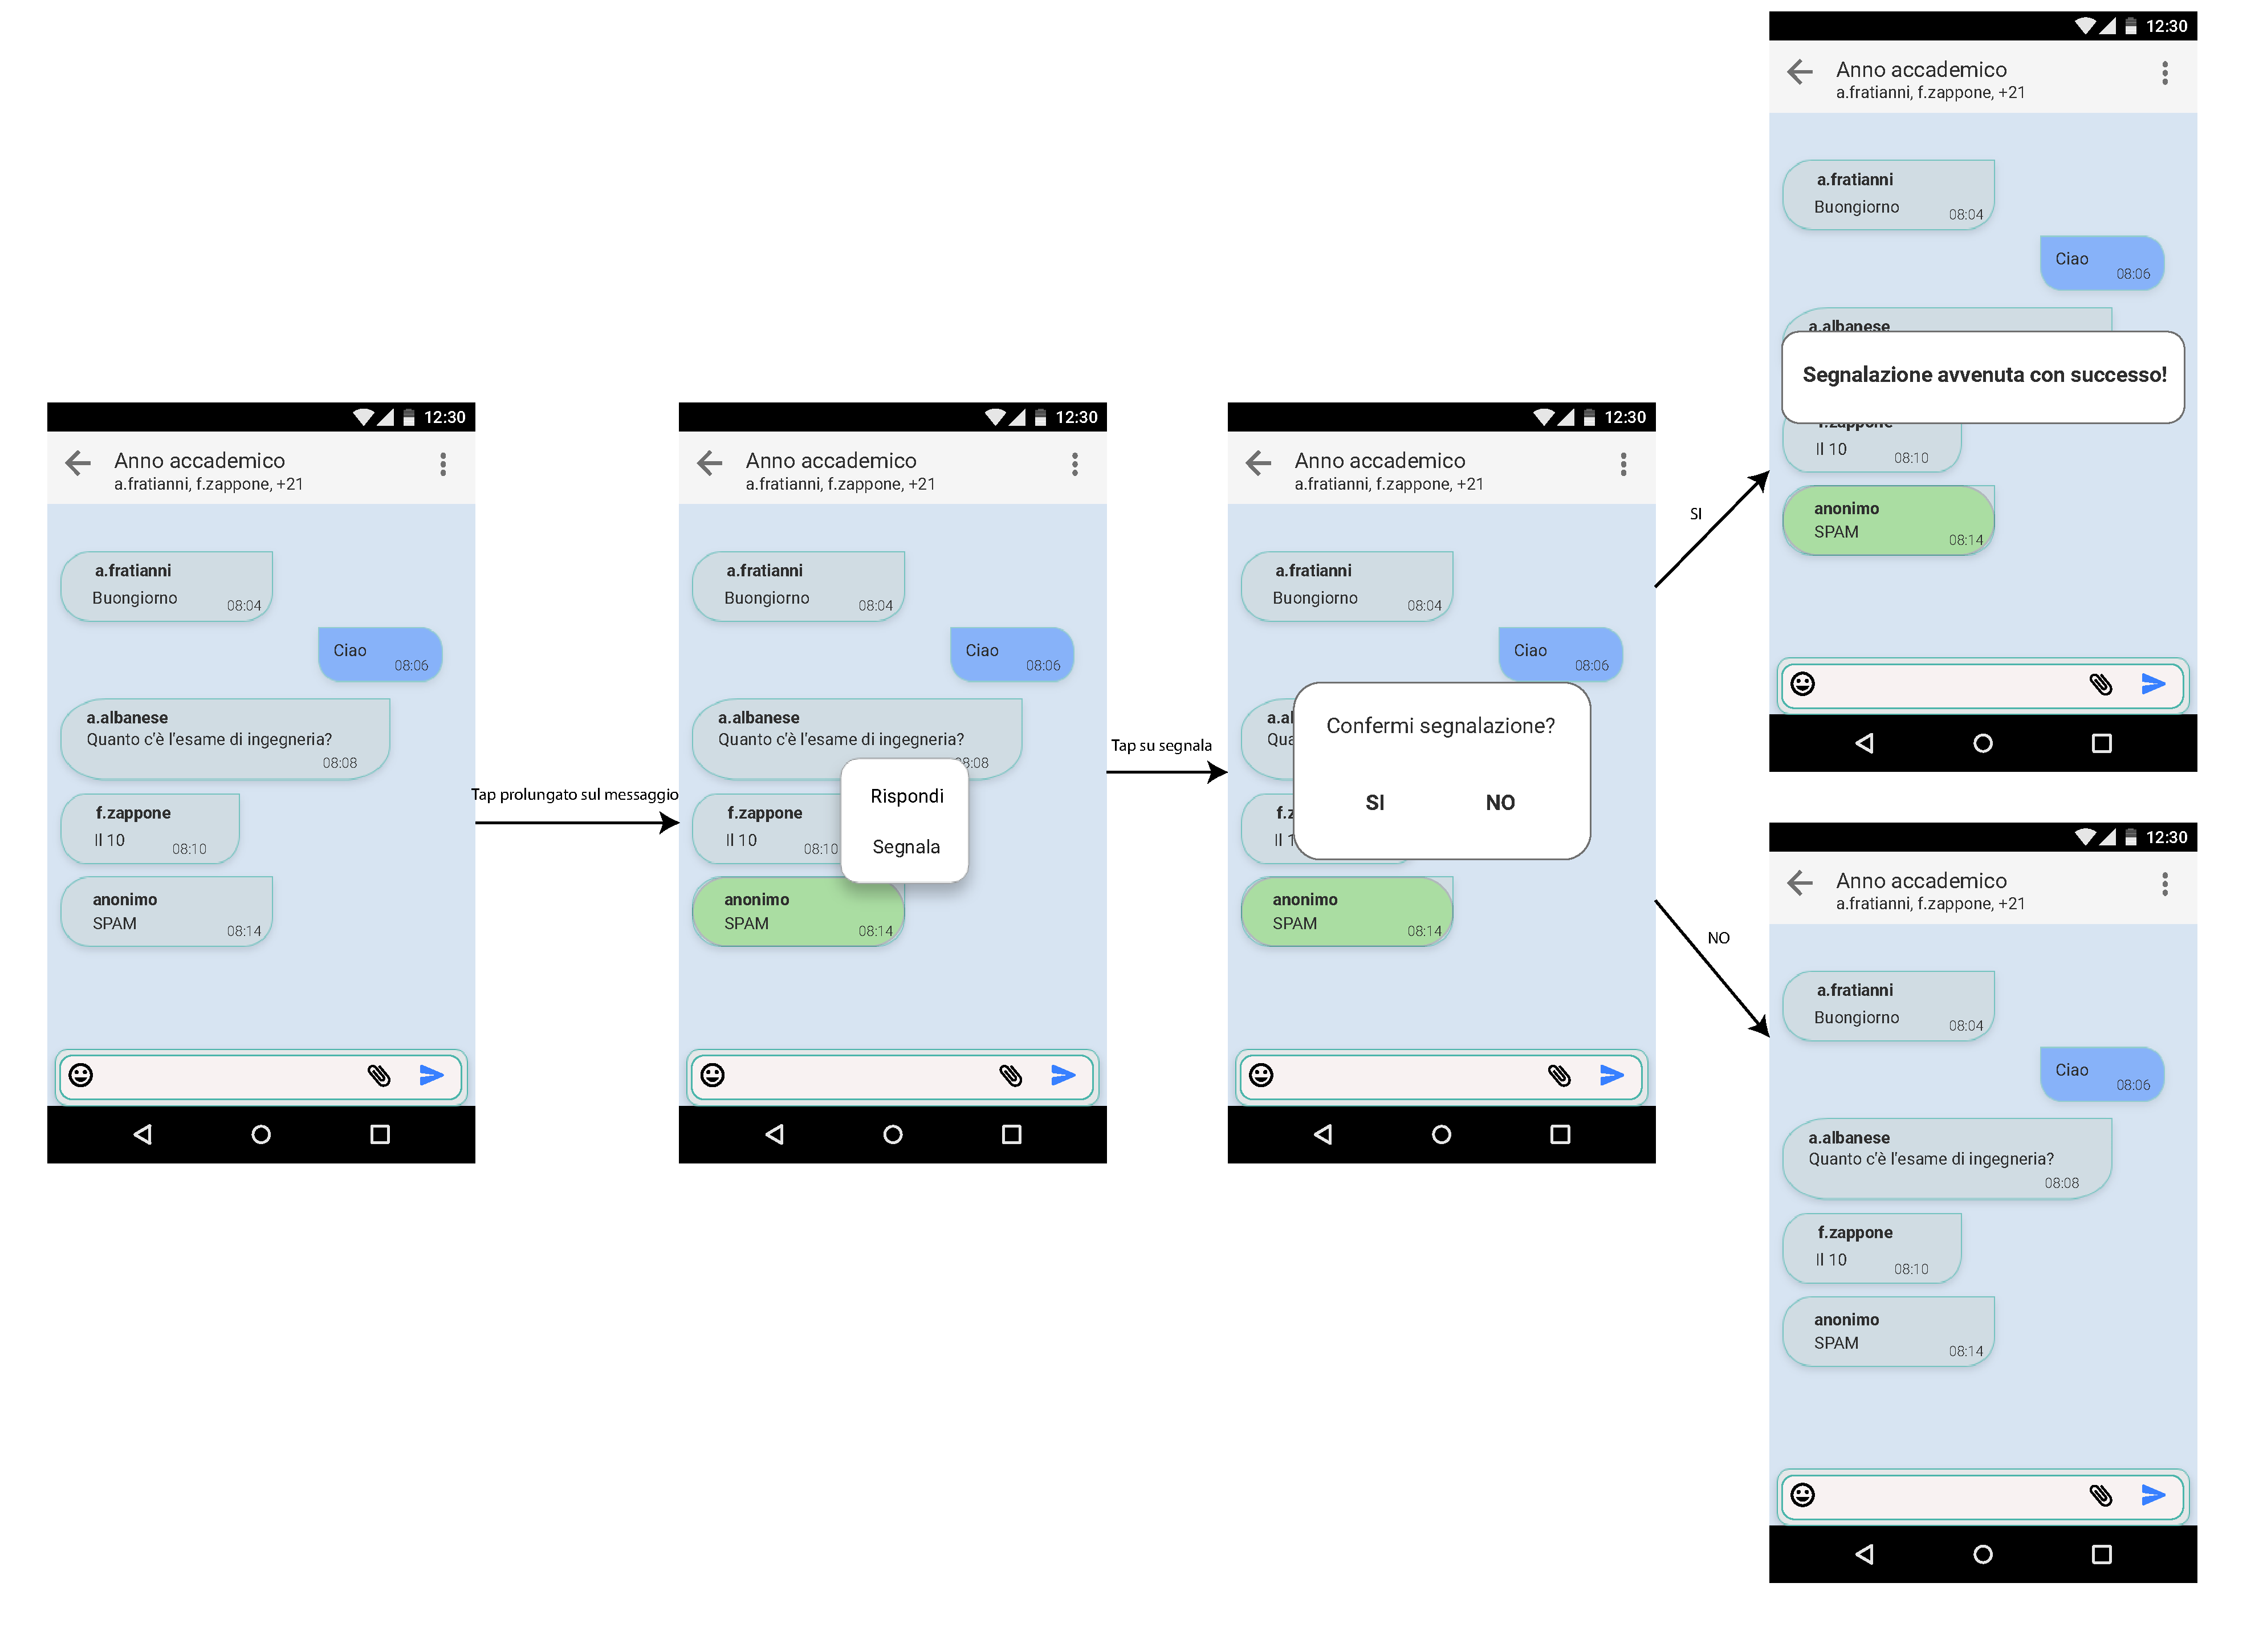
\includegraphics[width=0.9\textwidth]{imgs/gruppo6/activities/act_cus6_segnalazione_messaggio.pdf}
	\caption{CUS6 - Segnalazione messaggio}
	\label{fig:cus6}
\end{figure}

\begin{figure}
	\centering
	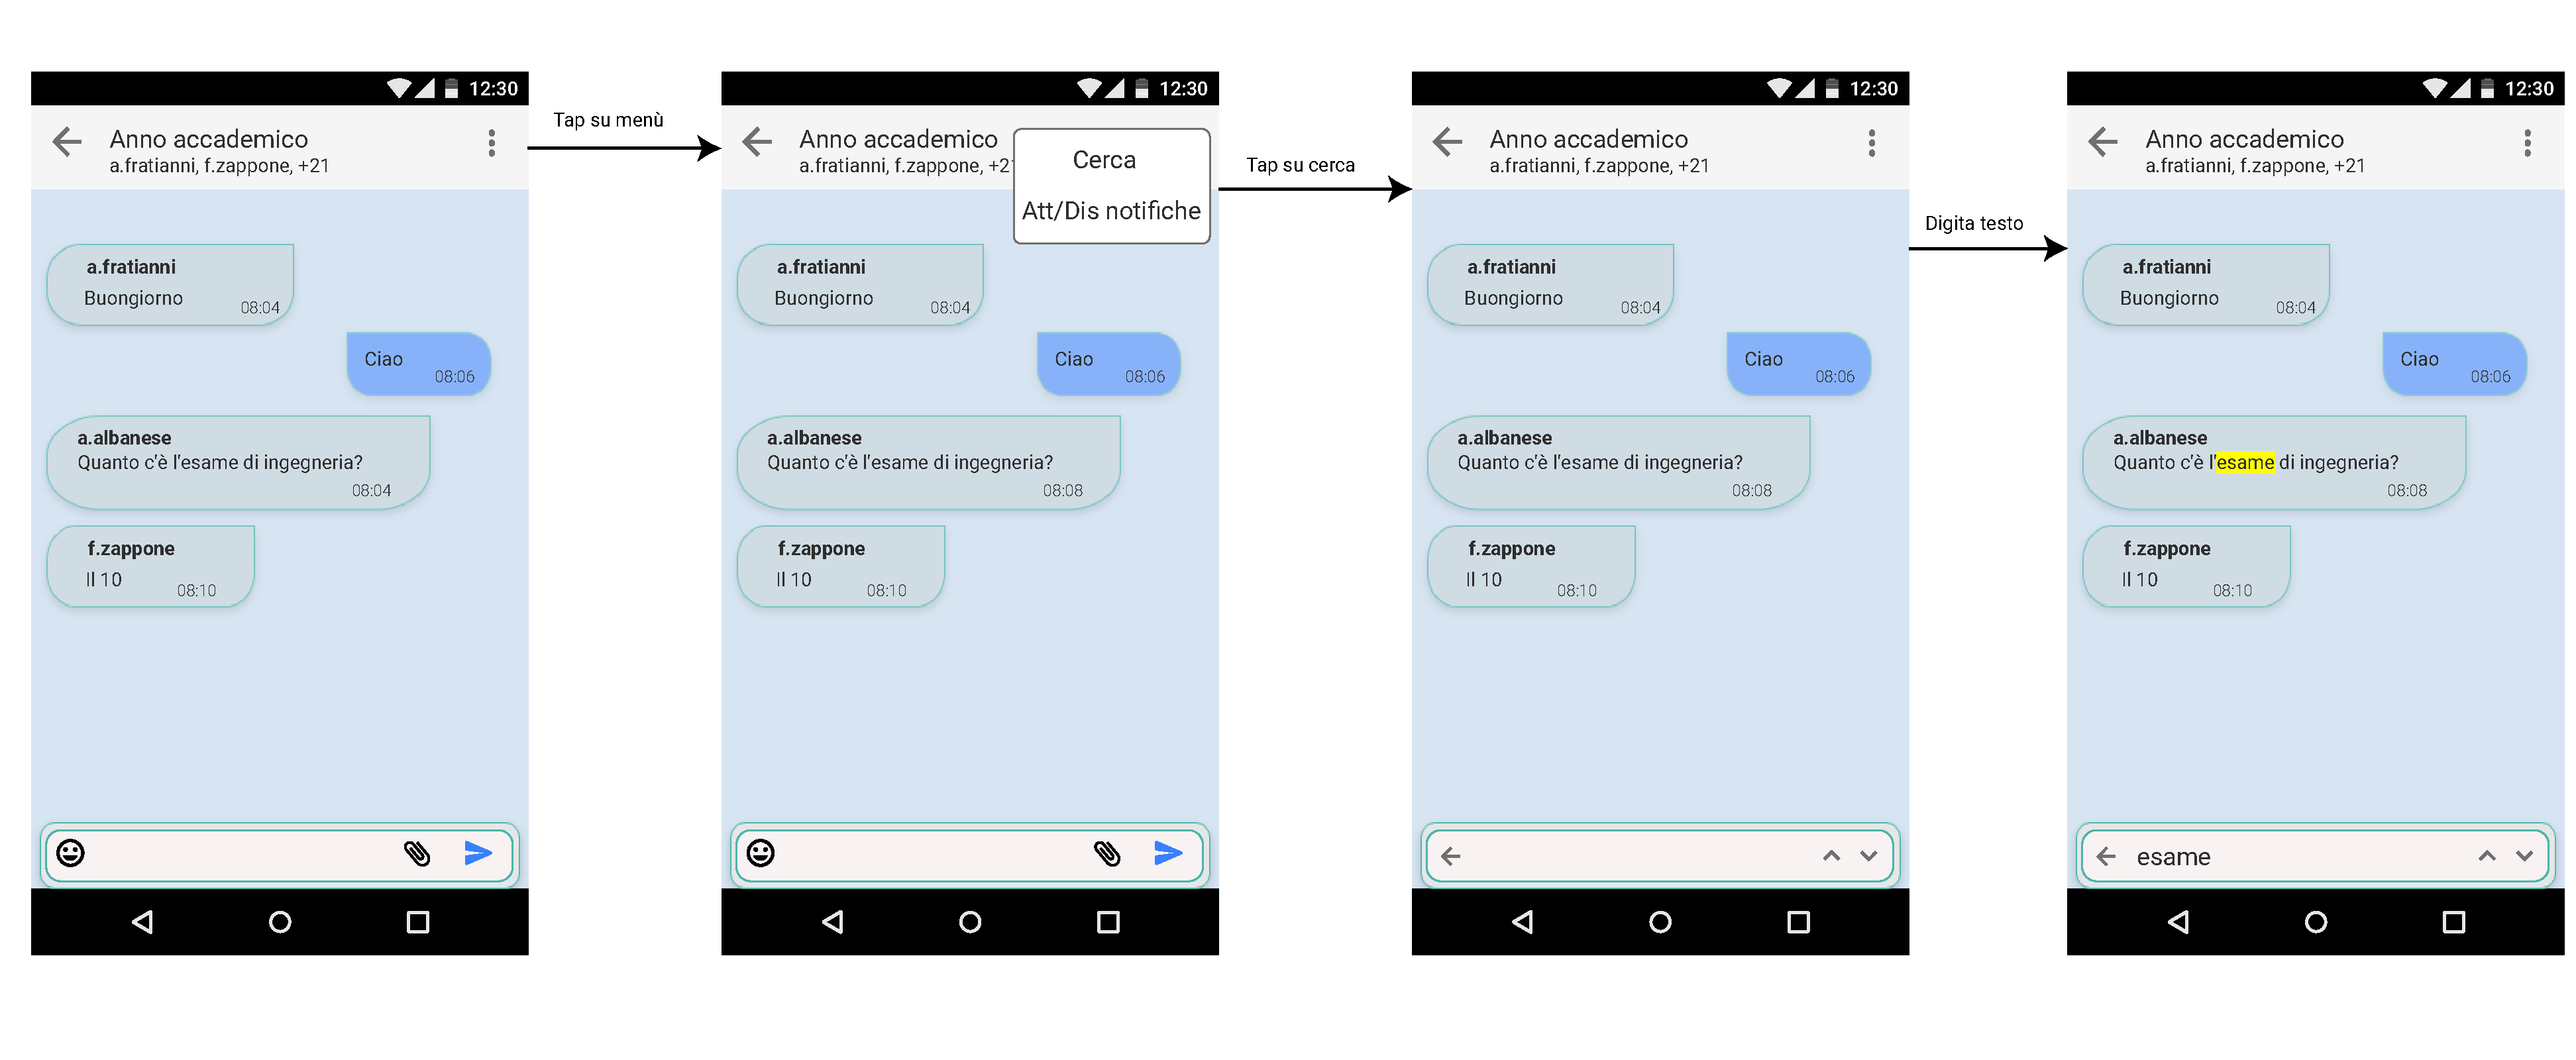
\includegraphics[width=0.9\textwidth]{imgs/gruppo6/activities/act_cus7_ricerca_testo_nella_chat.pdf}
	\caption{CUS7 - Ricerca testo nella chat}
	\label{fig:cus7}
\end{figure}

\begin{figure}
	\centering
	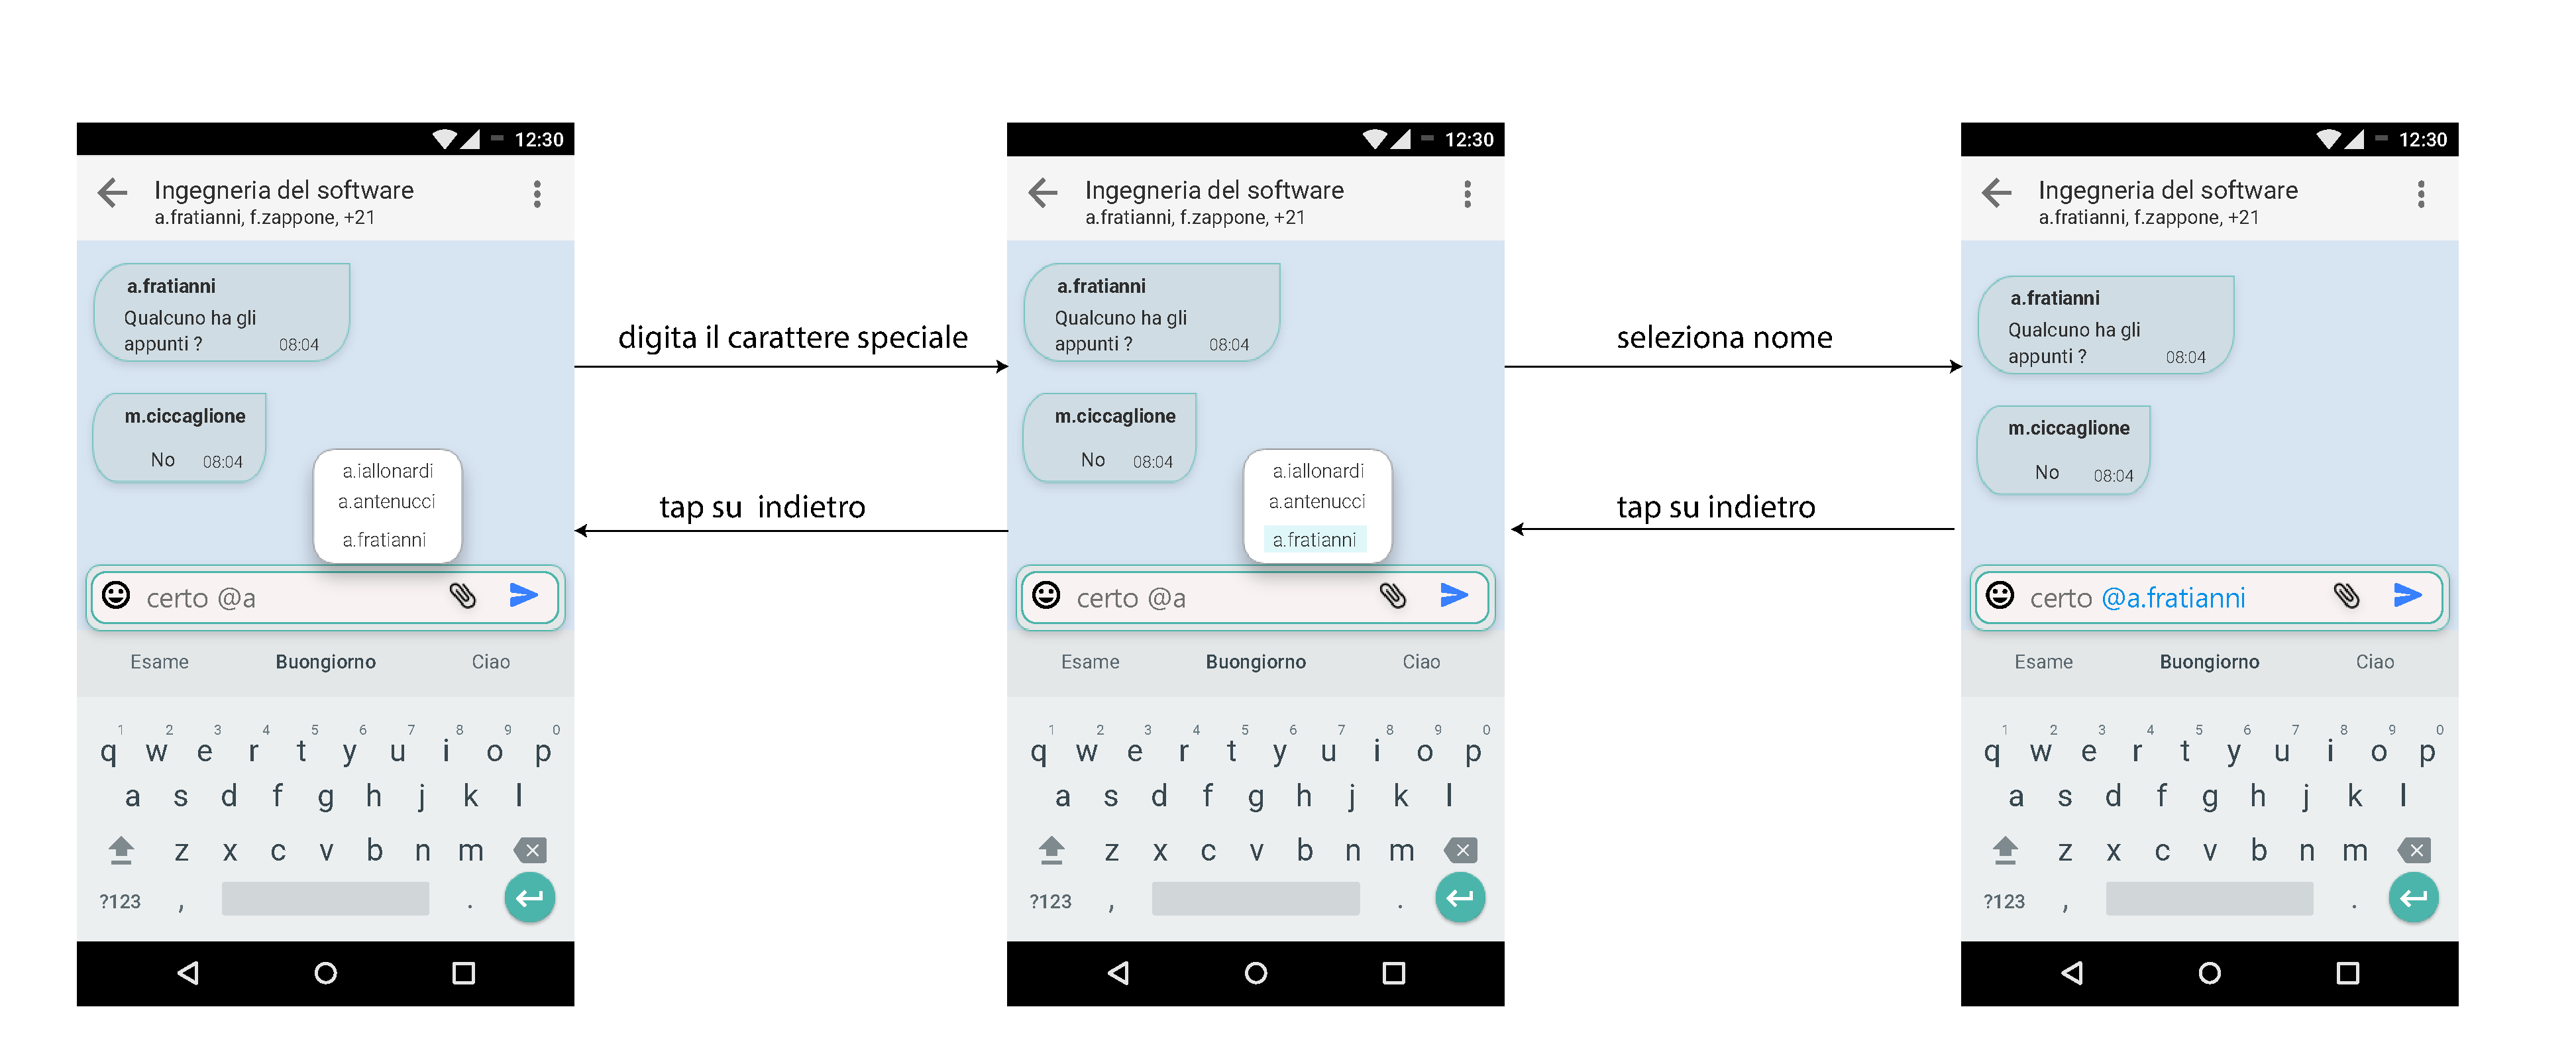
\includegraphics[width=0.9\textwidth]{imgs/gruppo6/activities/act_cus8_tag_membro_messaggio.pdf}
	\caption{CUS8 - Tag membro in messaggio}
	\label{fig:cus8}
\end{figure}

\begin{figure}
	\centering
	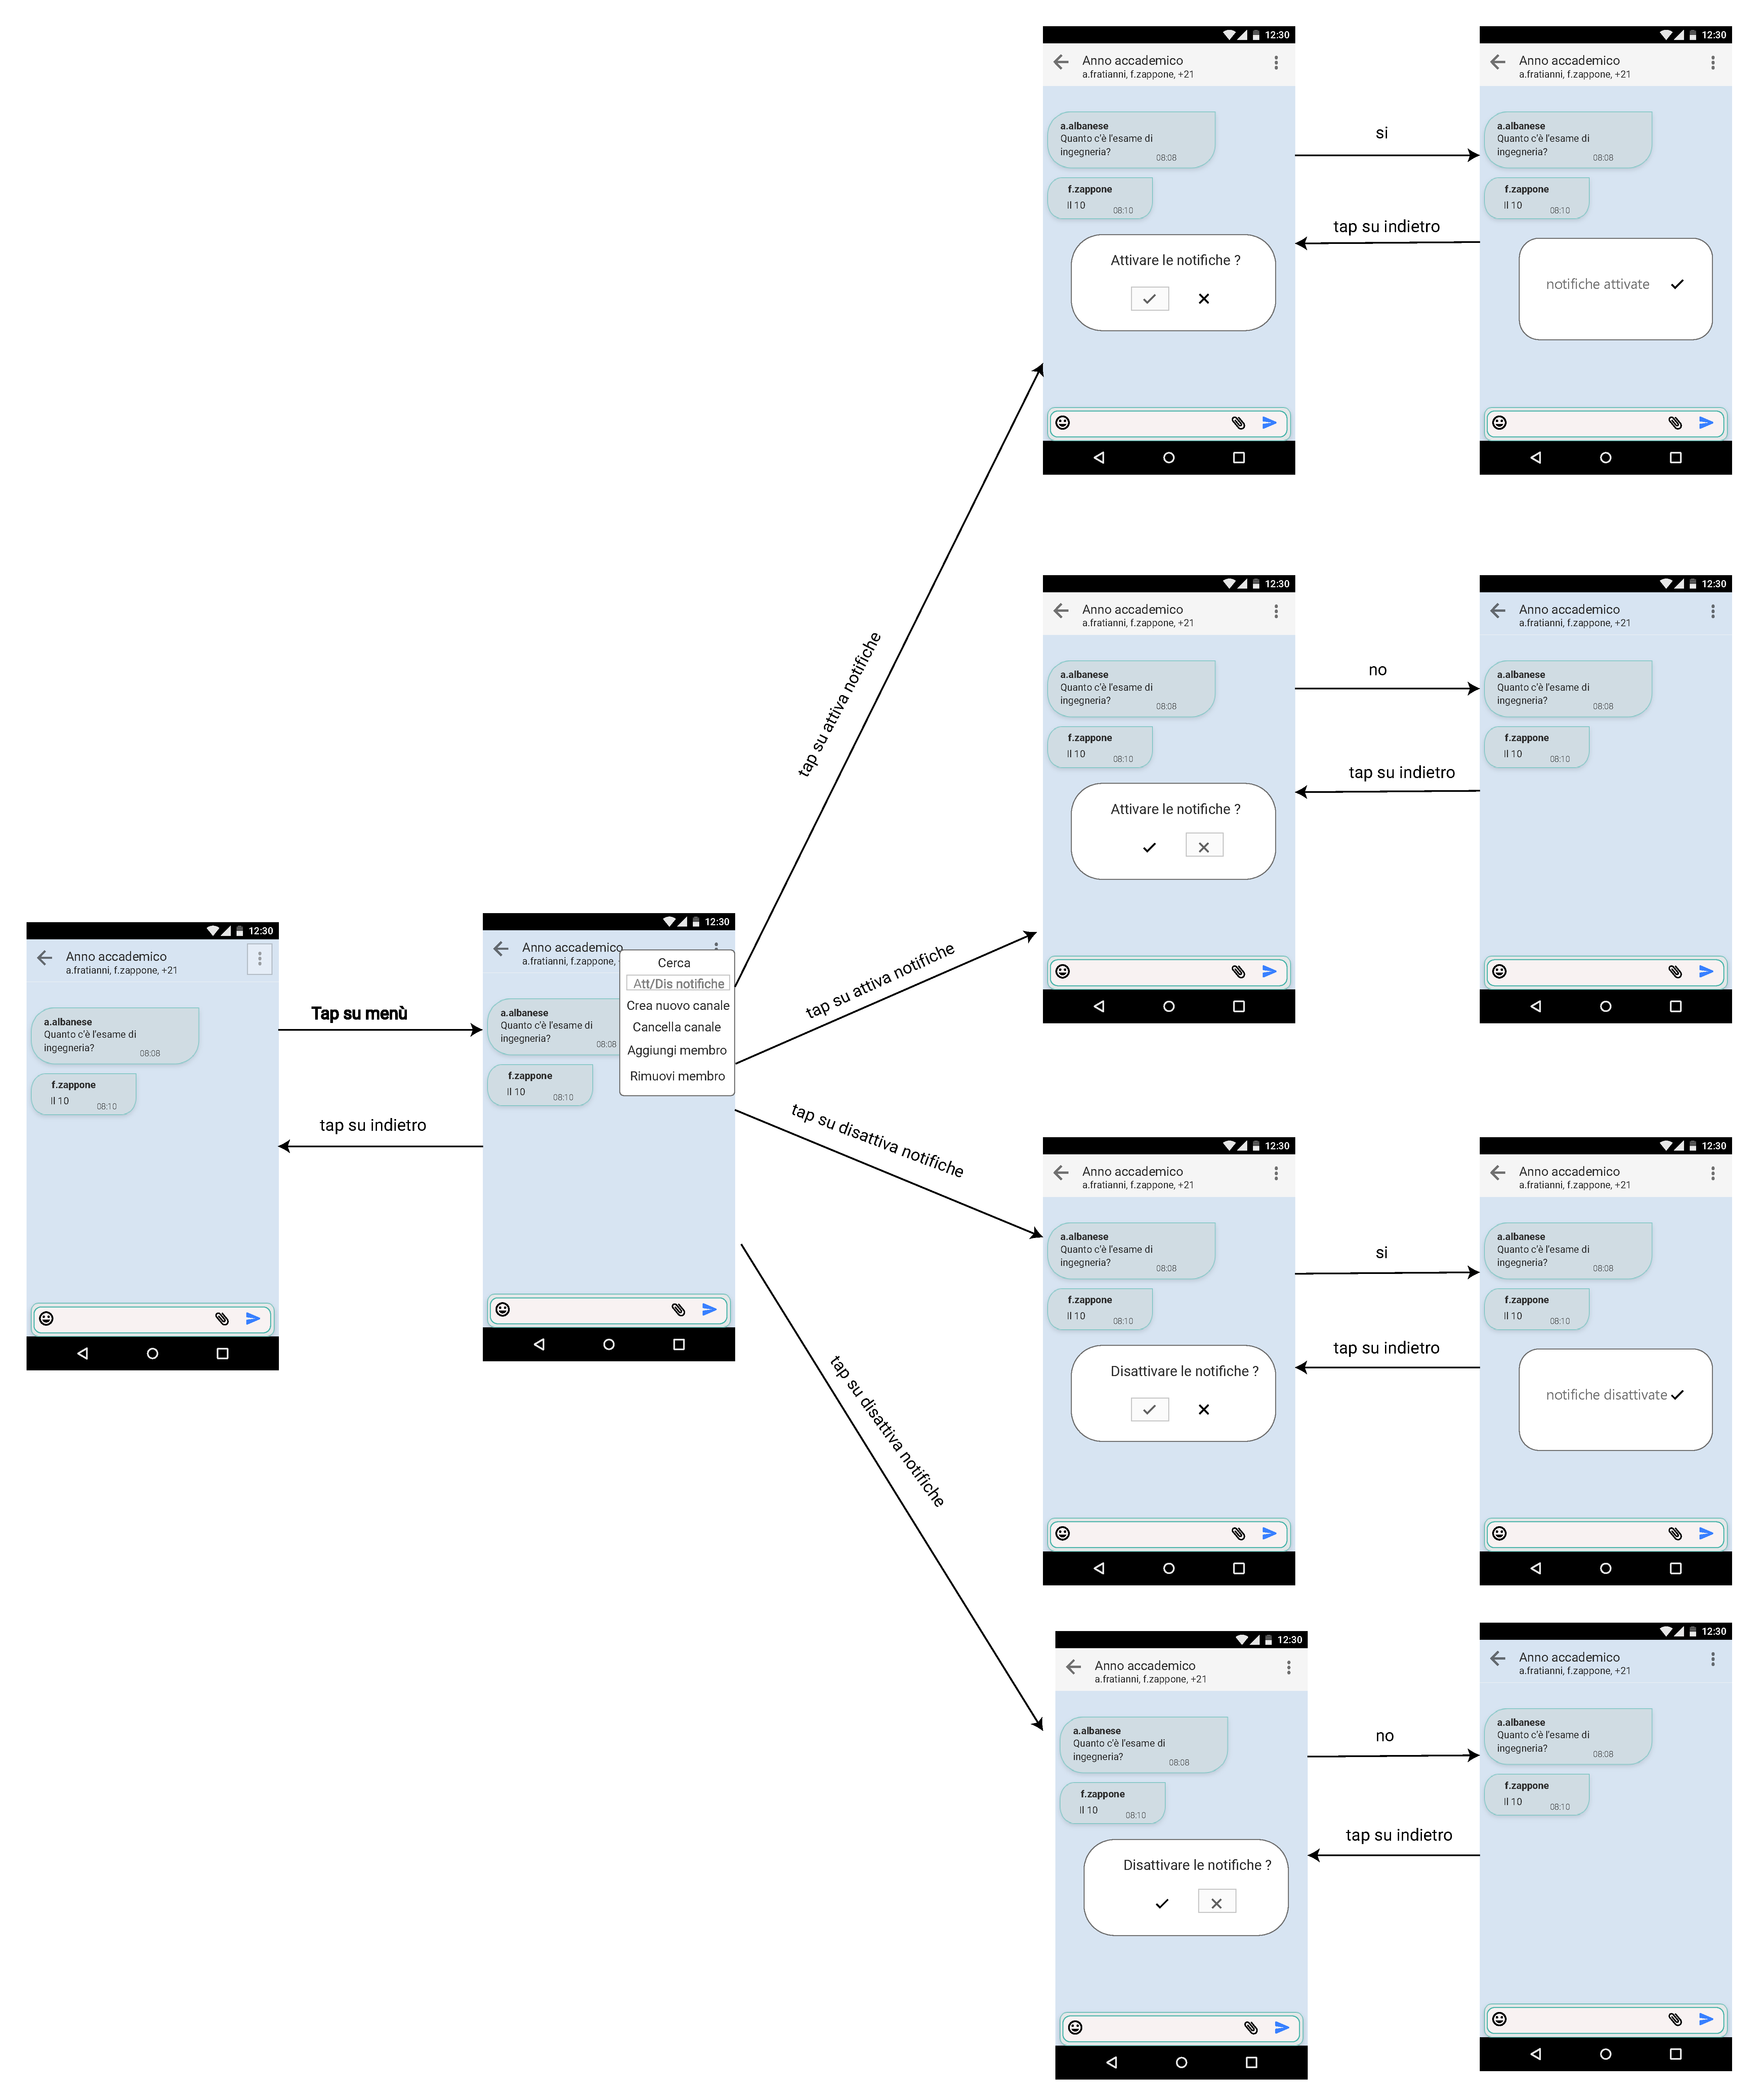
\includegraphics[width=0.9\textwidth]{imgs/gruppo6/activities/act_cus9_gestisci_notifiche_chat.pdf}
	\caption{CUS9 - Gestisci notifiche chat}
	\label{fig:cus9}
\end{figure}

\begin{figure}
	\centering
	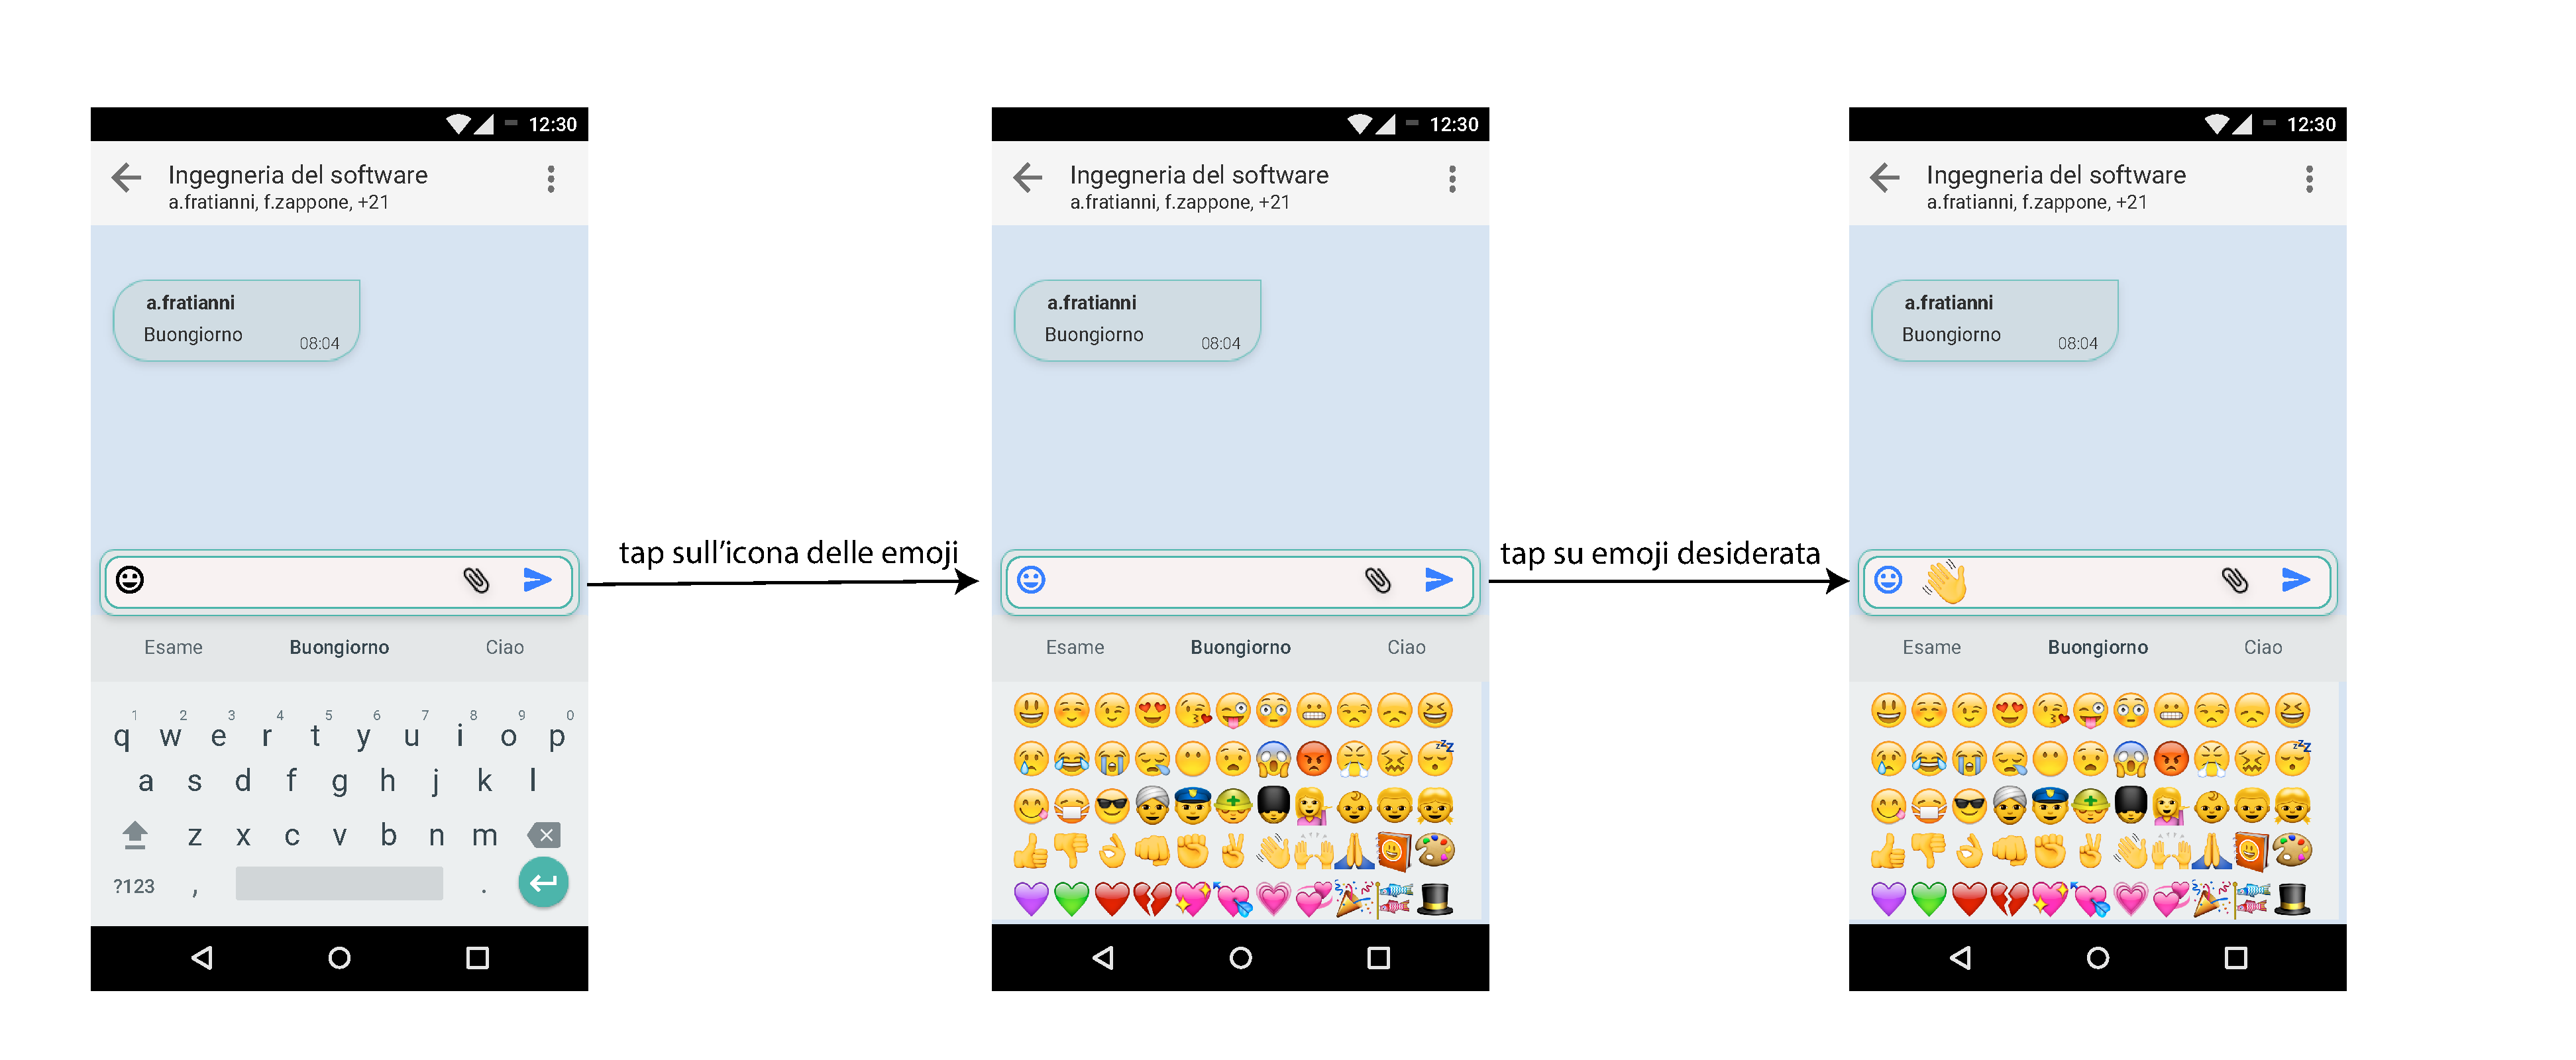
\includegraphics[width=0.9\textwidth]{imgs/gruppo6/activities/act_cus10_seleziona_emoji.pdf}
	\caption{CUS10 - Selezione emoji}
	\label{fig:cus10}
\end{figure}

\begin{figure}
	\centering
	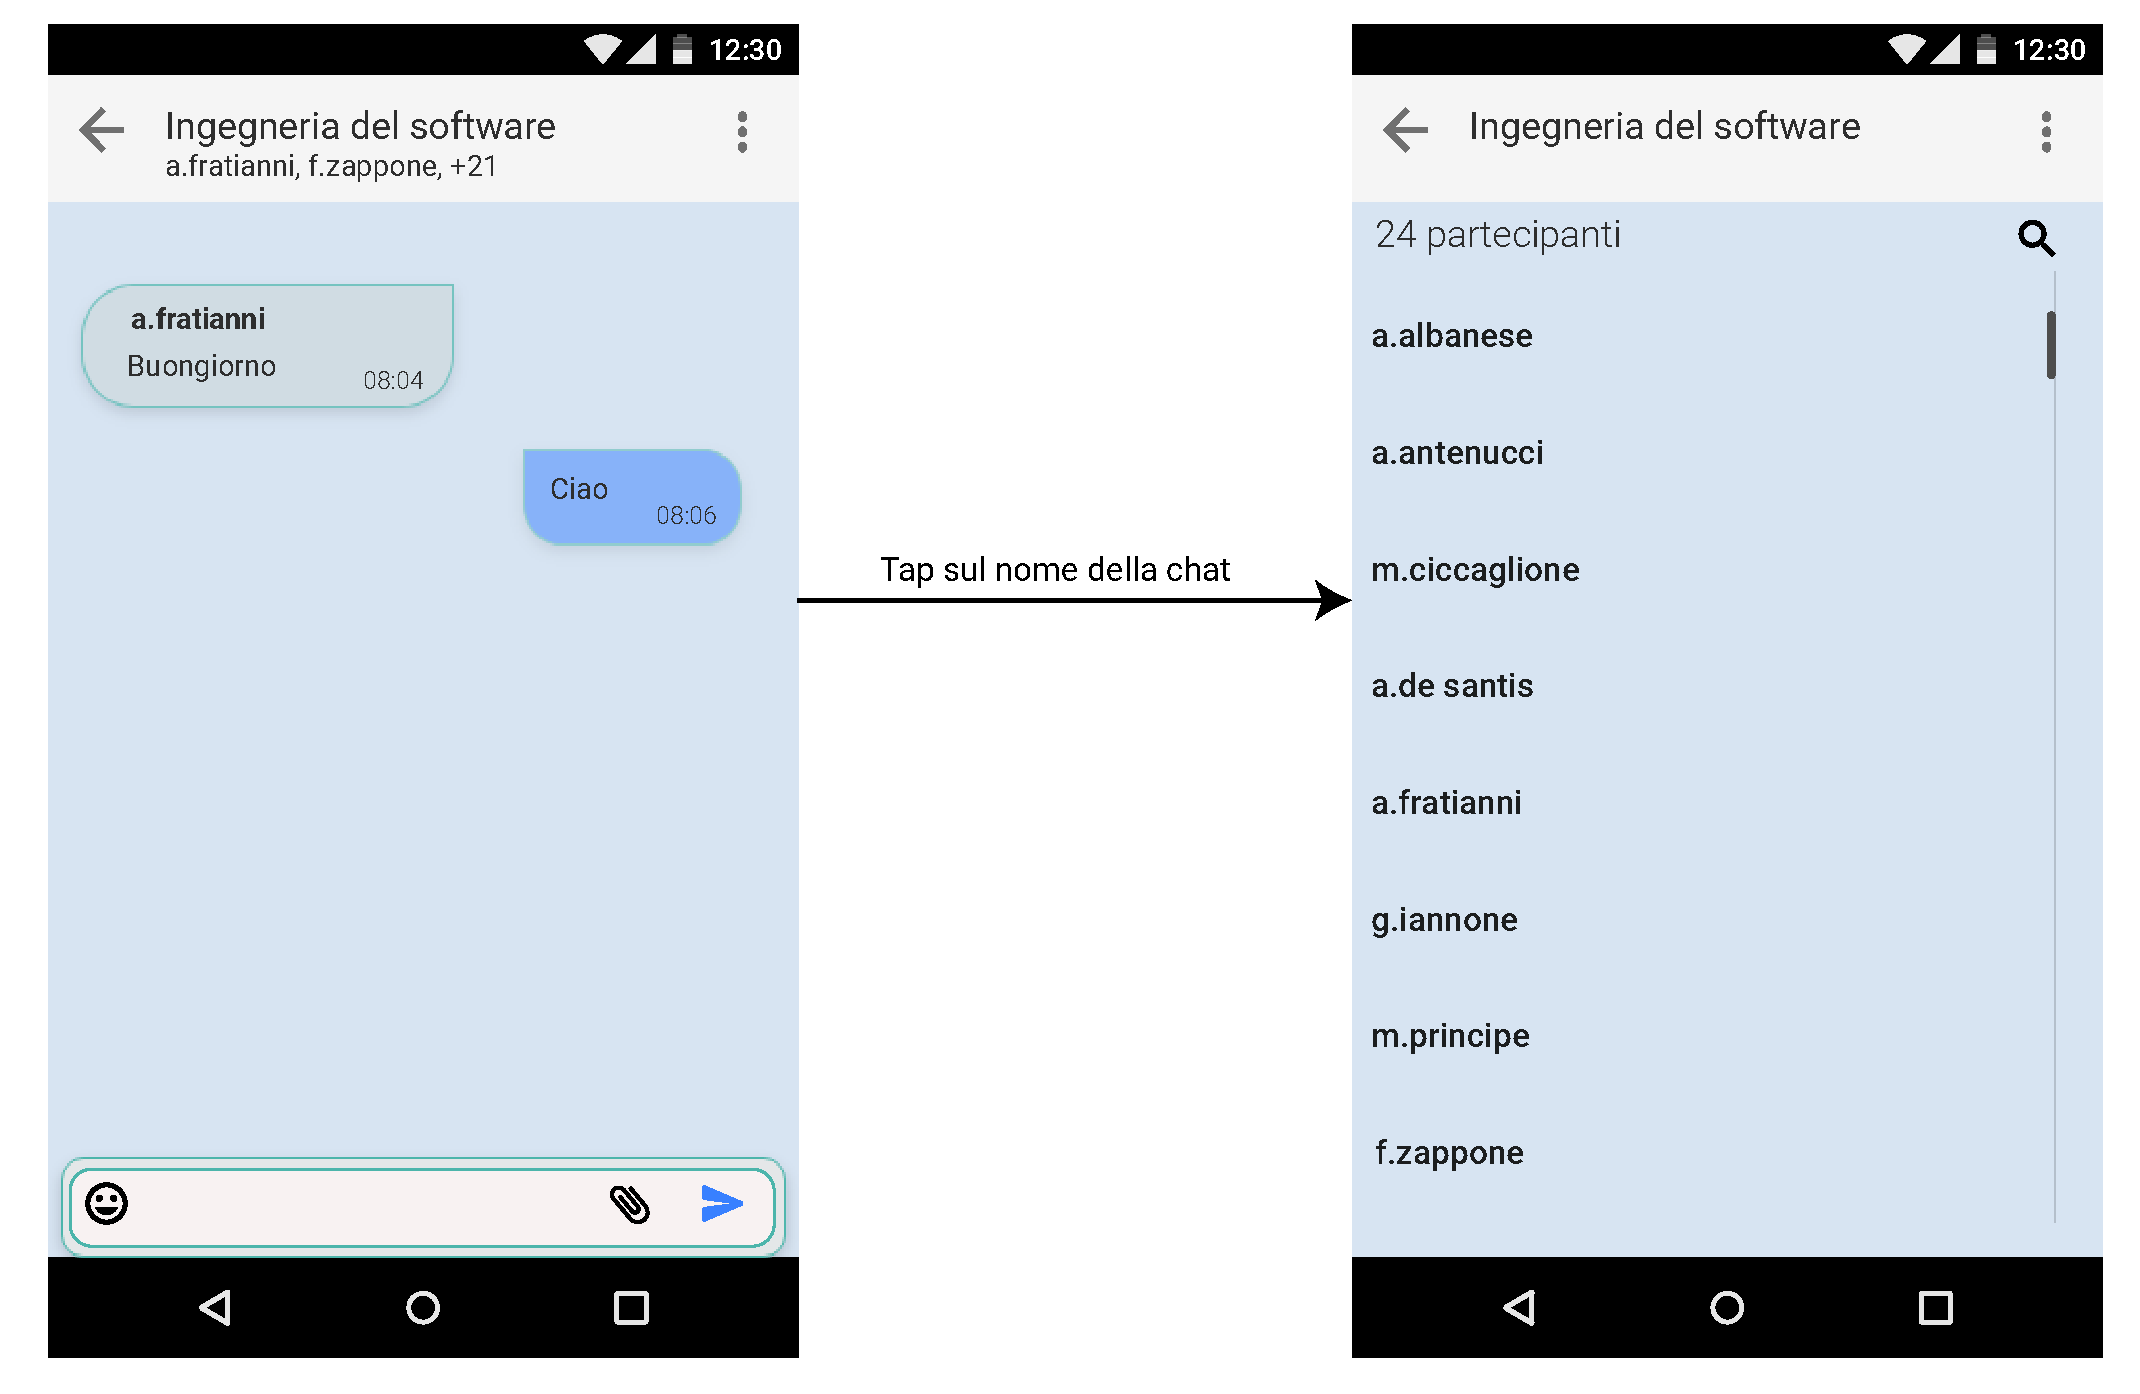
\includegraphics[width=0.9\textwidth]{imgs/gruppo6/activities/act_cus11_elenco_membri.pdf}
	\caption{CUS11 - Visualizza elenco membri chat}
	\label{fig:cus11}
\end{figure}
%%% END activities chat studenti %%%

%%% START activities chat docenti %%%
\pagebreak
\begin{figure}
\subsection{Activities relative alla chat dell'App Docenti}
	\centering
	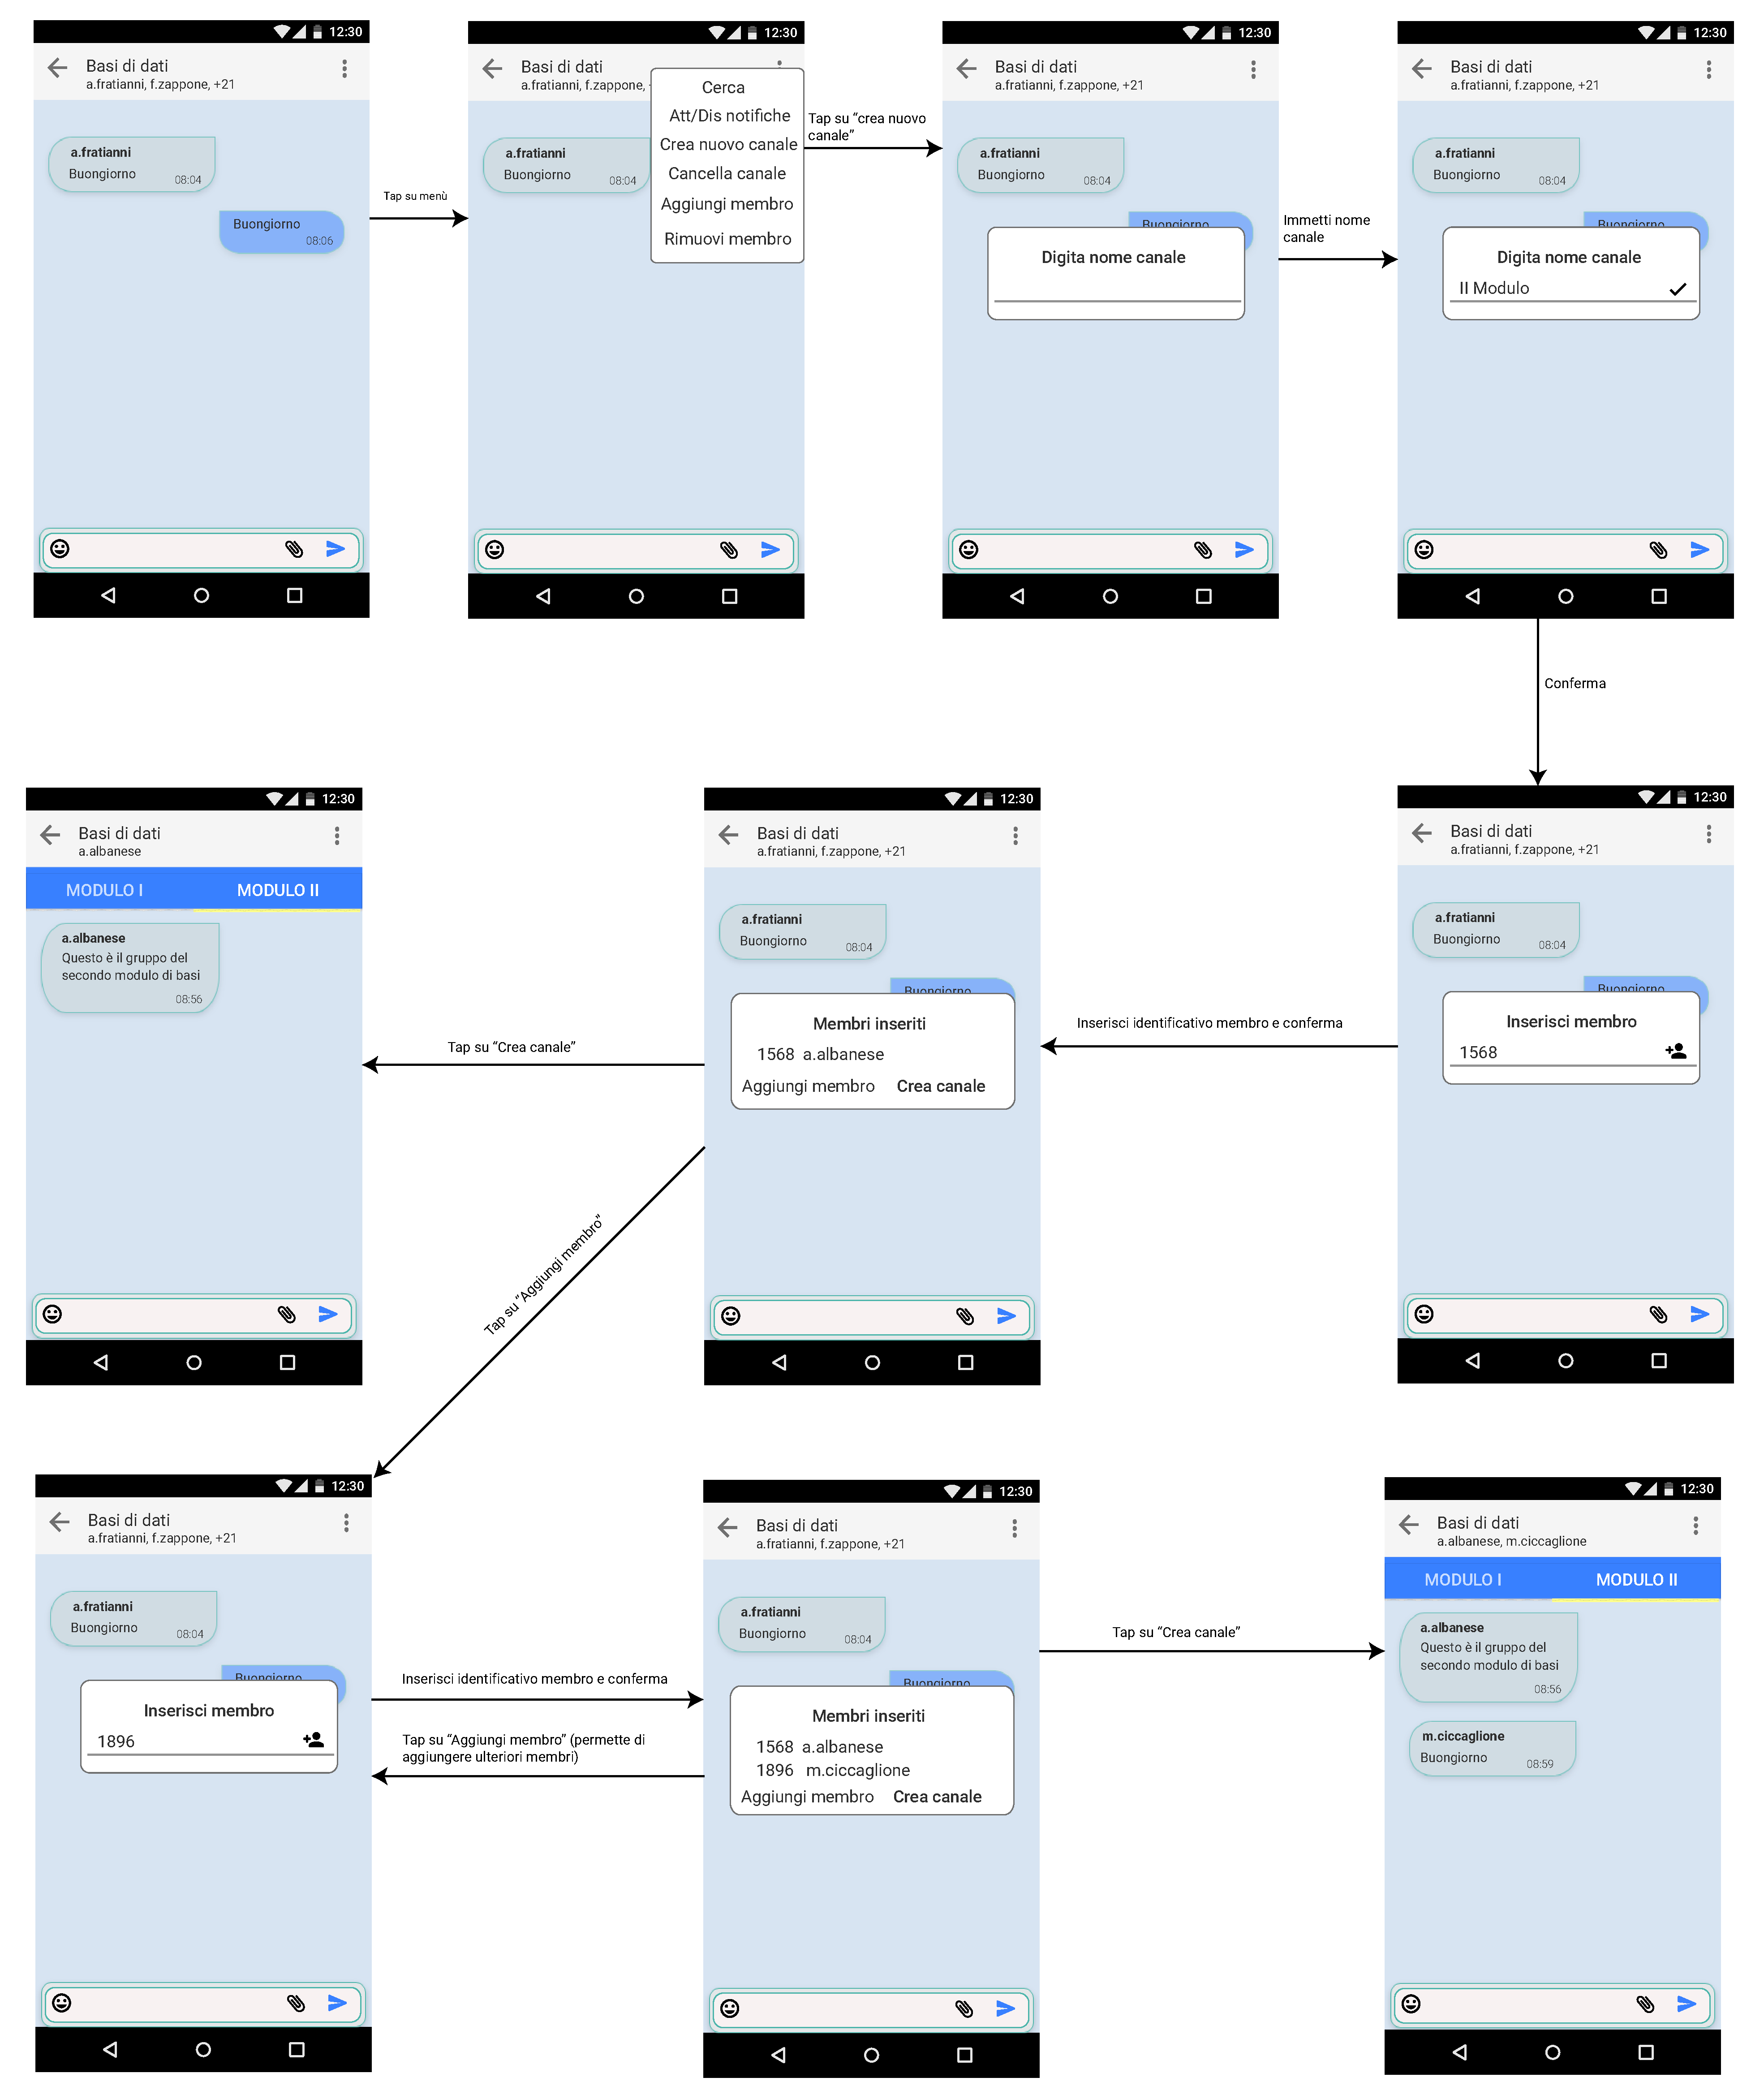
\includegraphics[width=0.9\textwidth]{imgs/gruppo6/activities/act_cud1_creazione_canale.pdf}
	\caption{CUD1 - Creazione canale}
	\label{fig:cud1}
\end{figure}

\begin{figure}
	\centering
	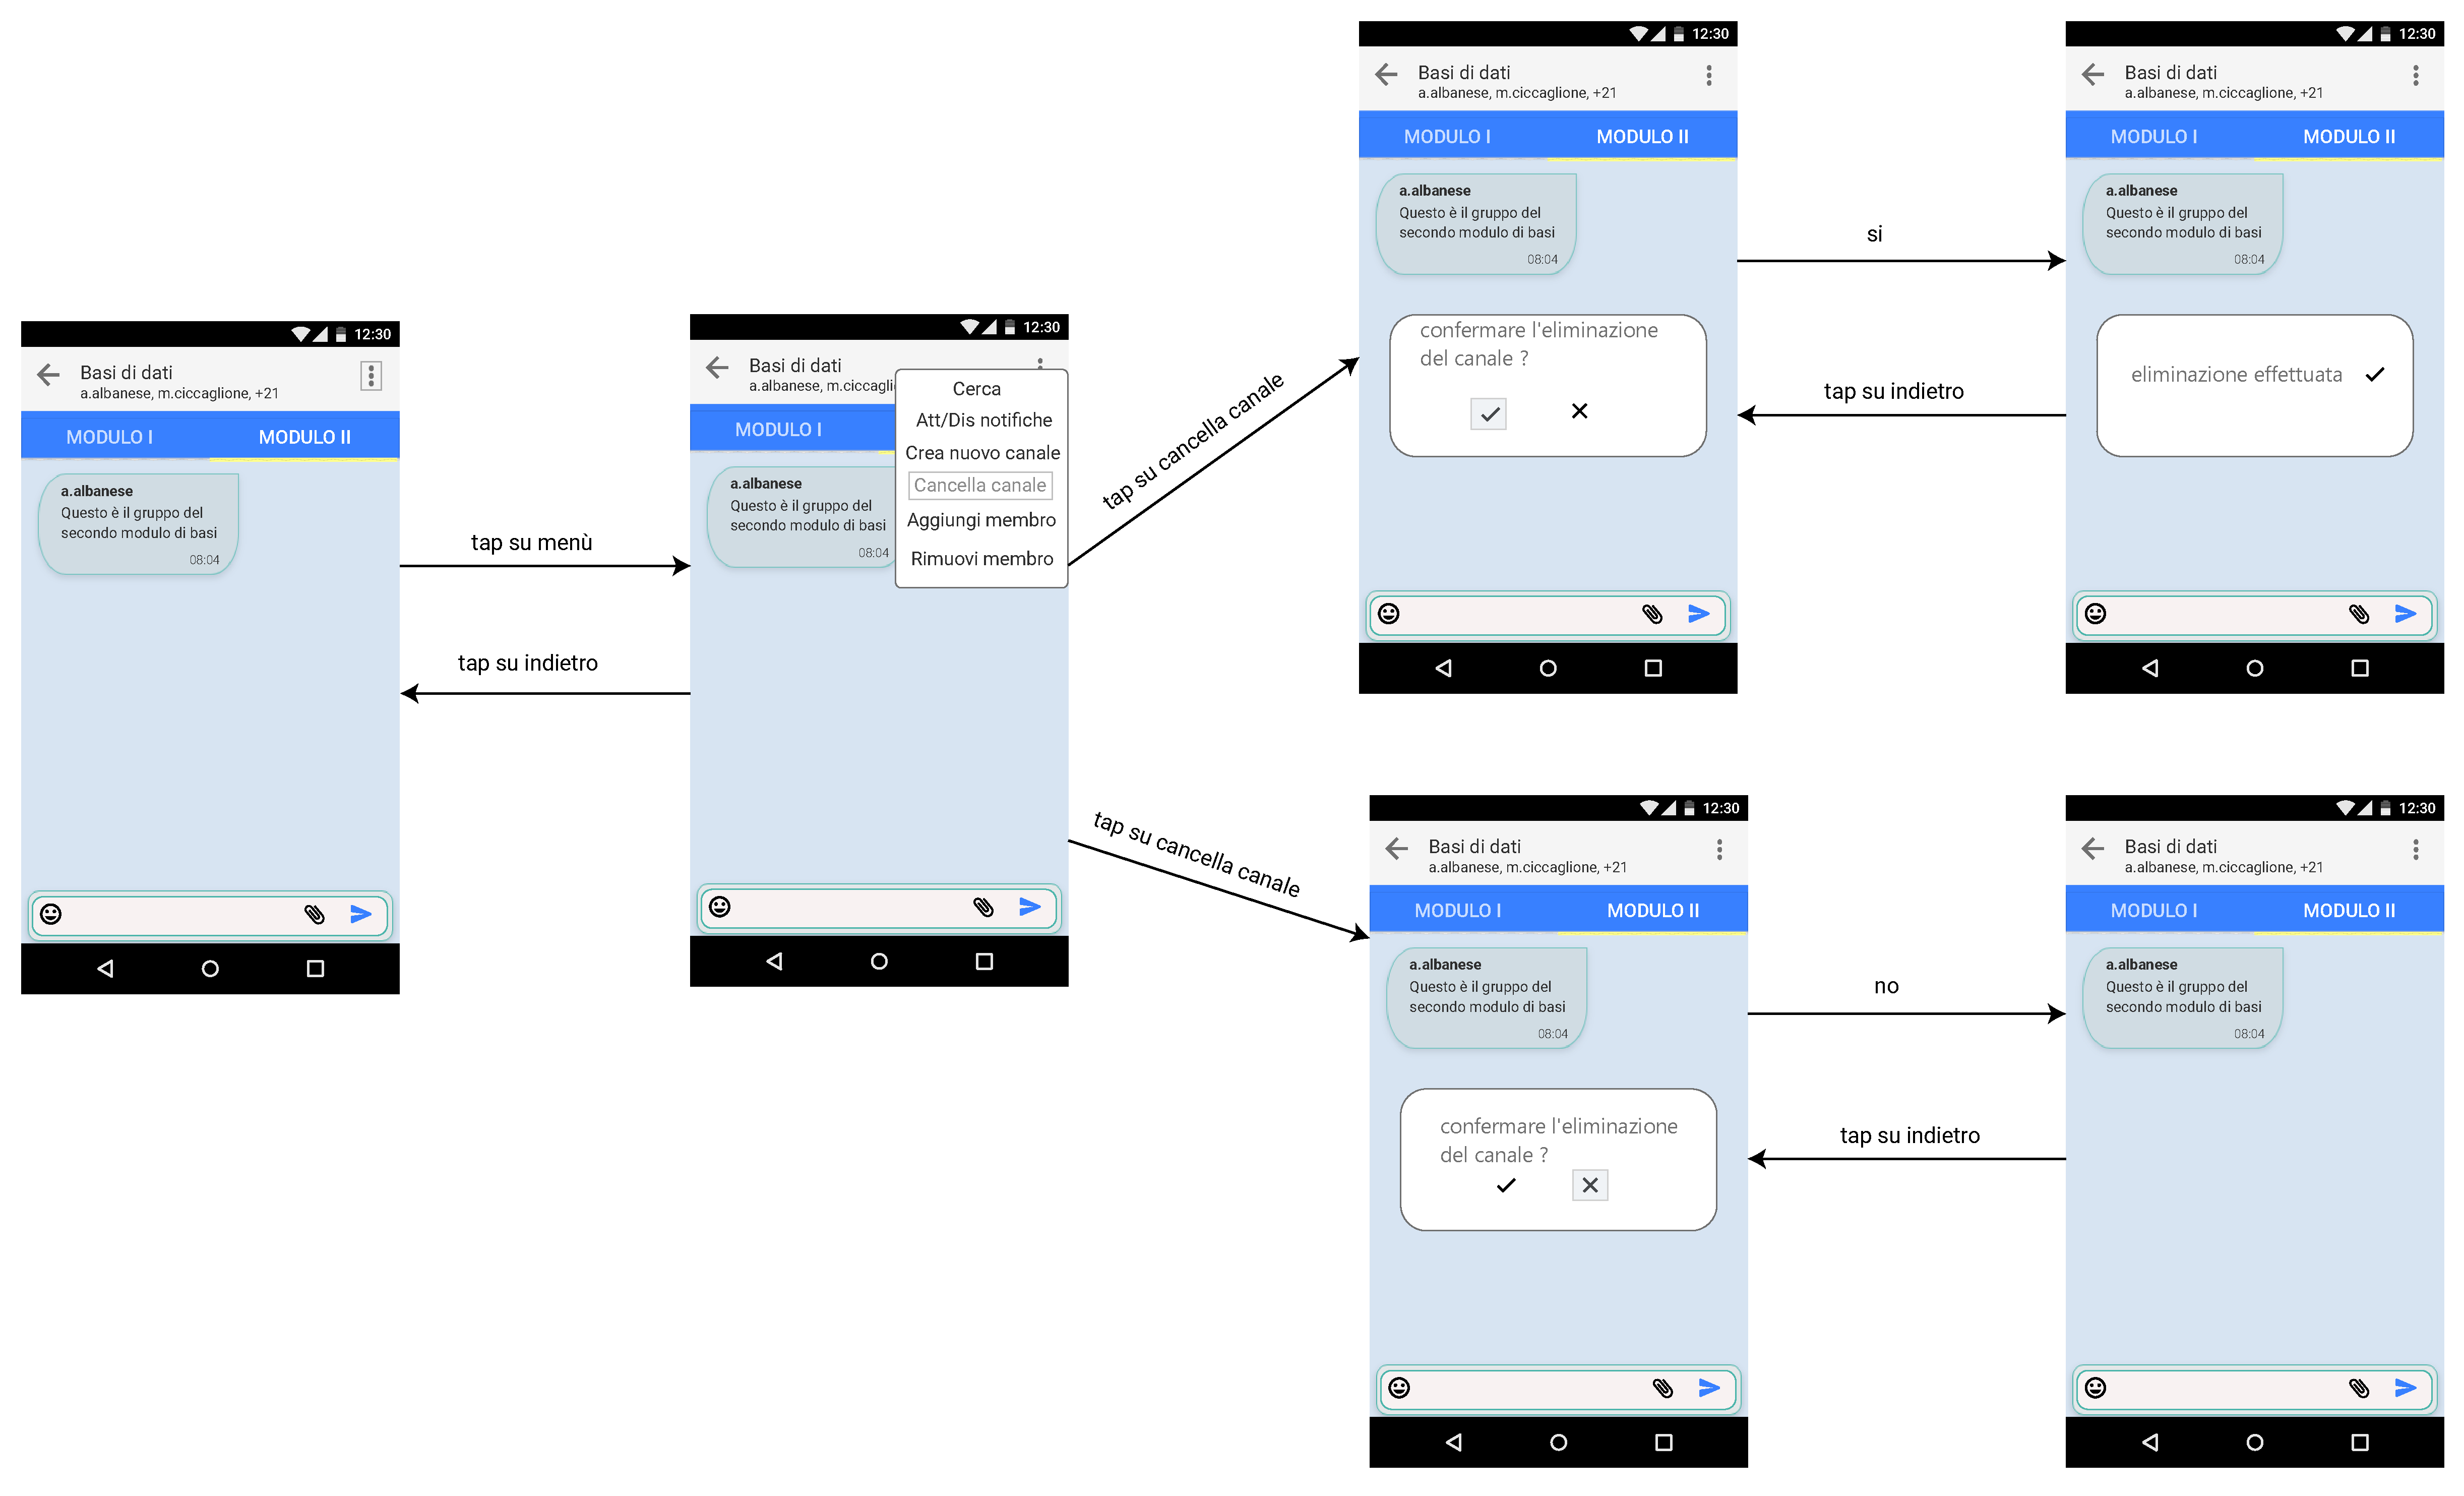
\includegraphics[width=0.9\textwidth]{imgs/gruppo6/activities/act_cud2_cancella_canale.pdf}
	\caption{CUD2 - Cancellazione canale}
	\label{fig:cud2}
\end{figure}

\begin{figure}
	\centering
	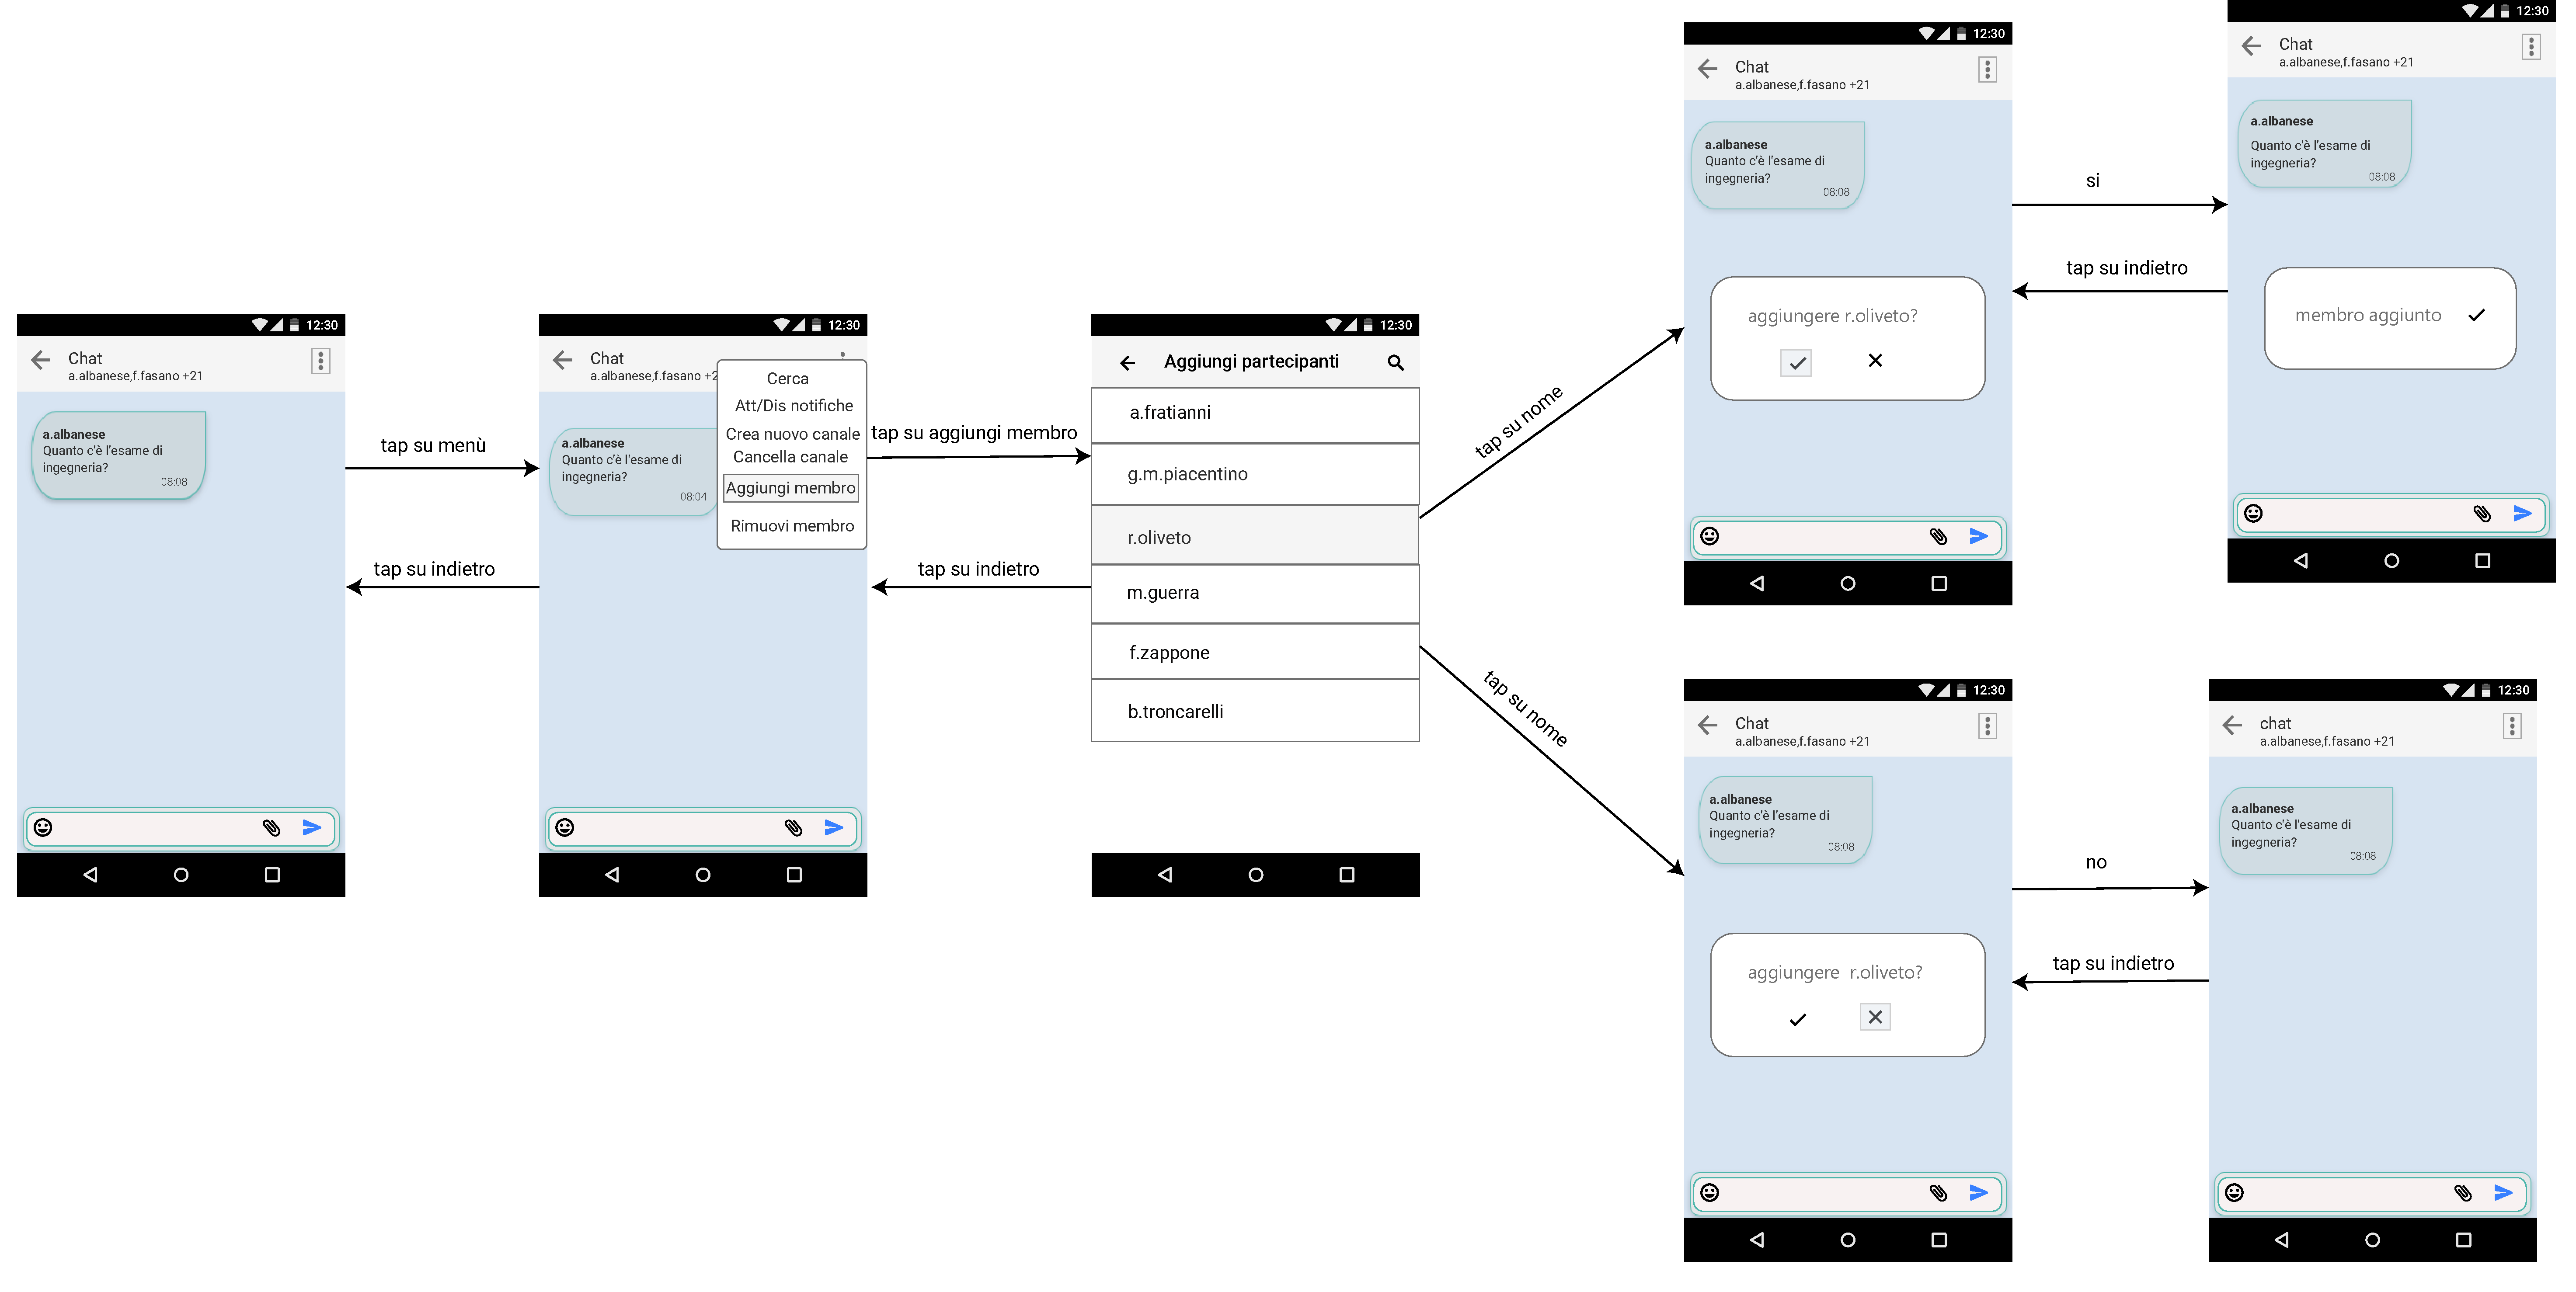
\includegraphics[width=0.9\textwidth]{imgs/gruppo6/activities/act_cud3_aggiungi_membro_chat.pdf}
	\caption{CUD3 - Aggiungi membro ad un canale}
	\label{fig:cud3}
\end{figure}

\begin{figure}
	\centering
	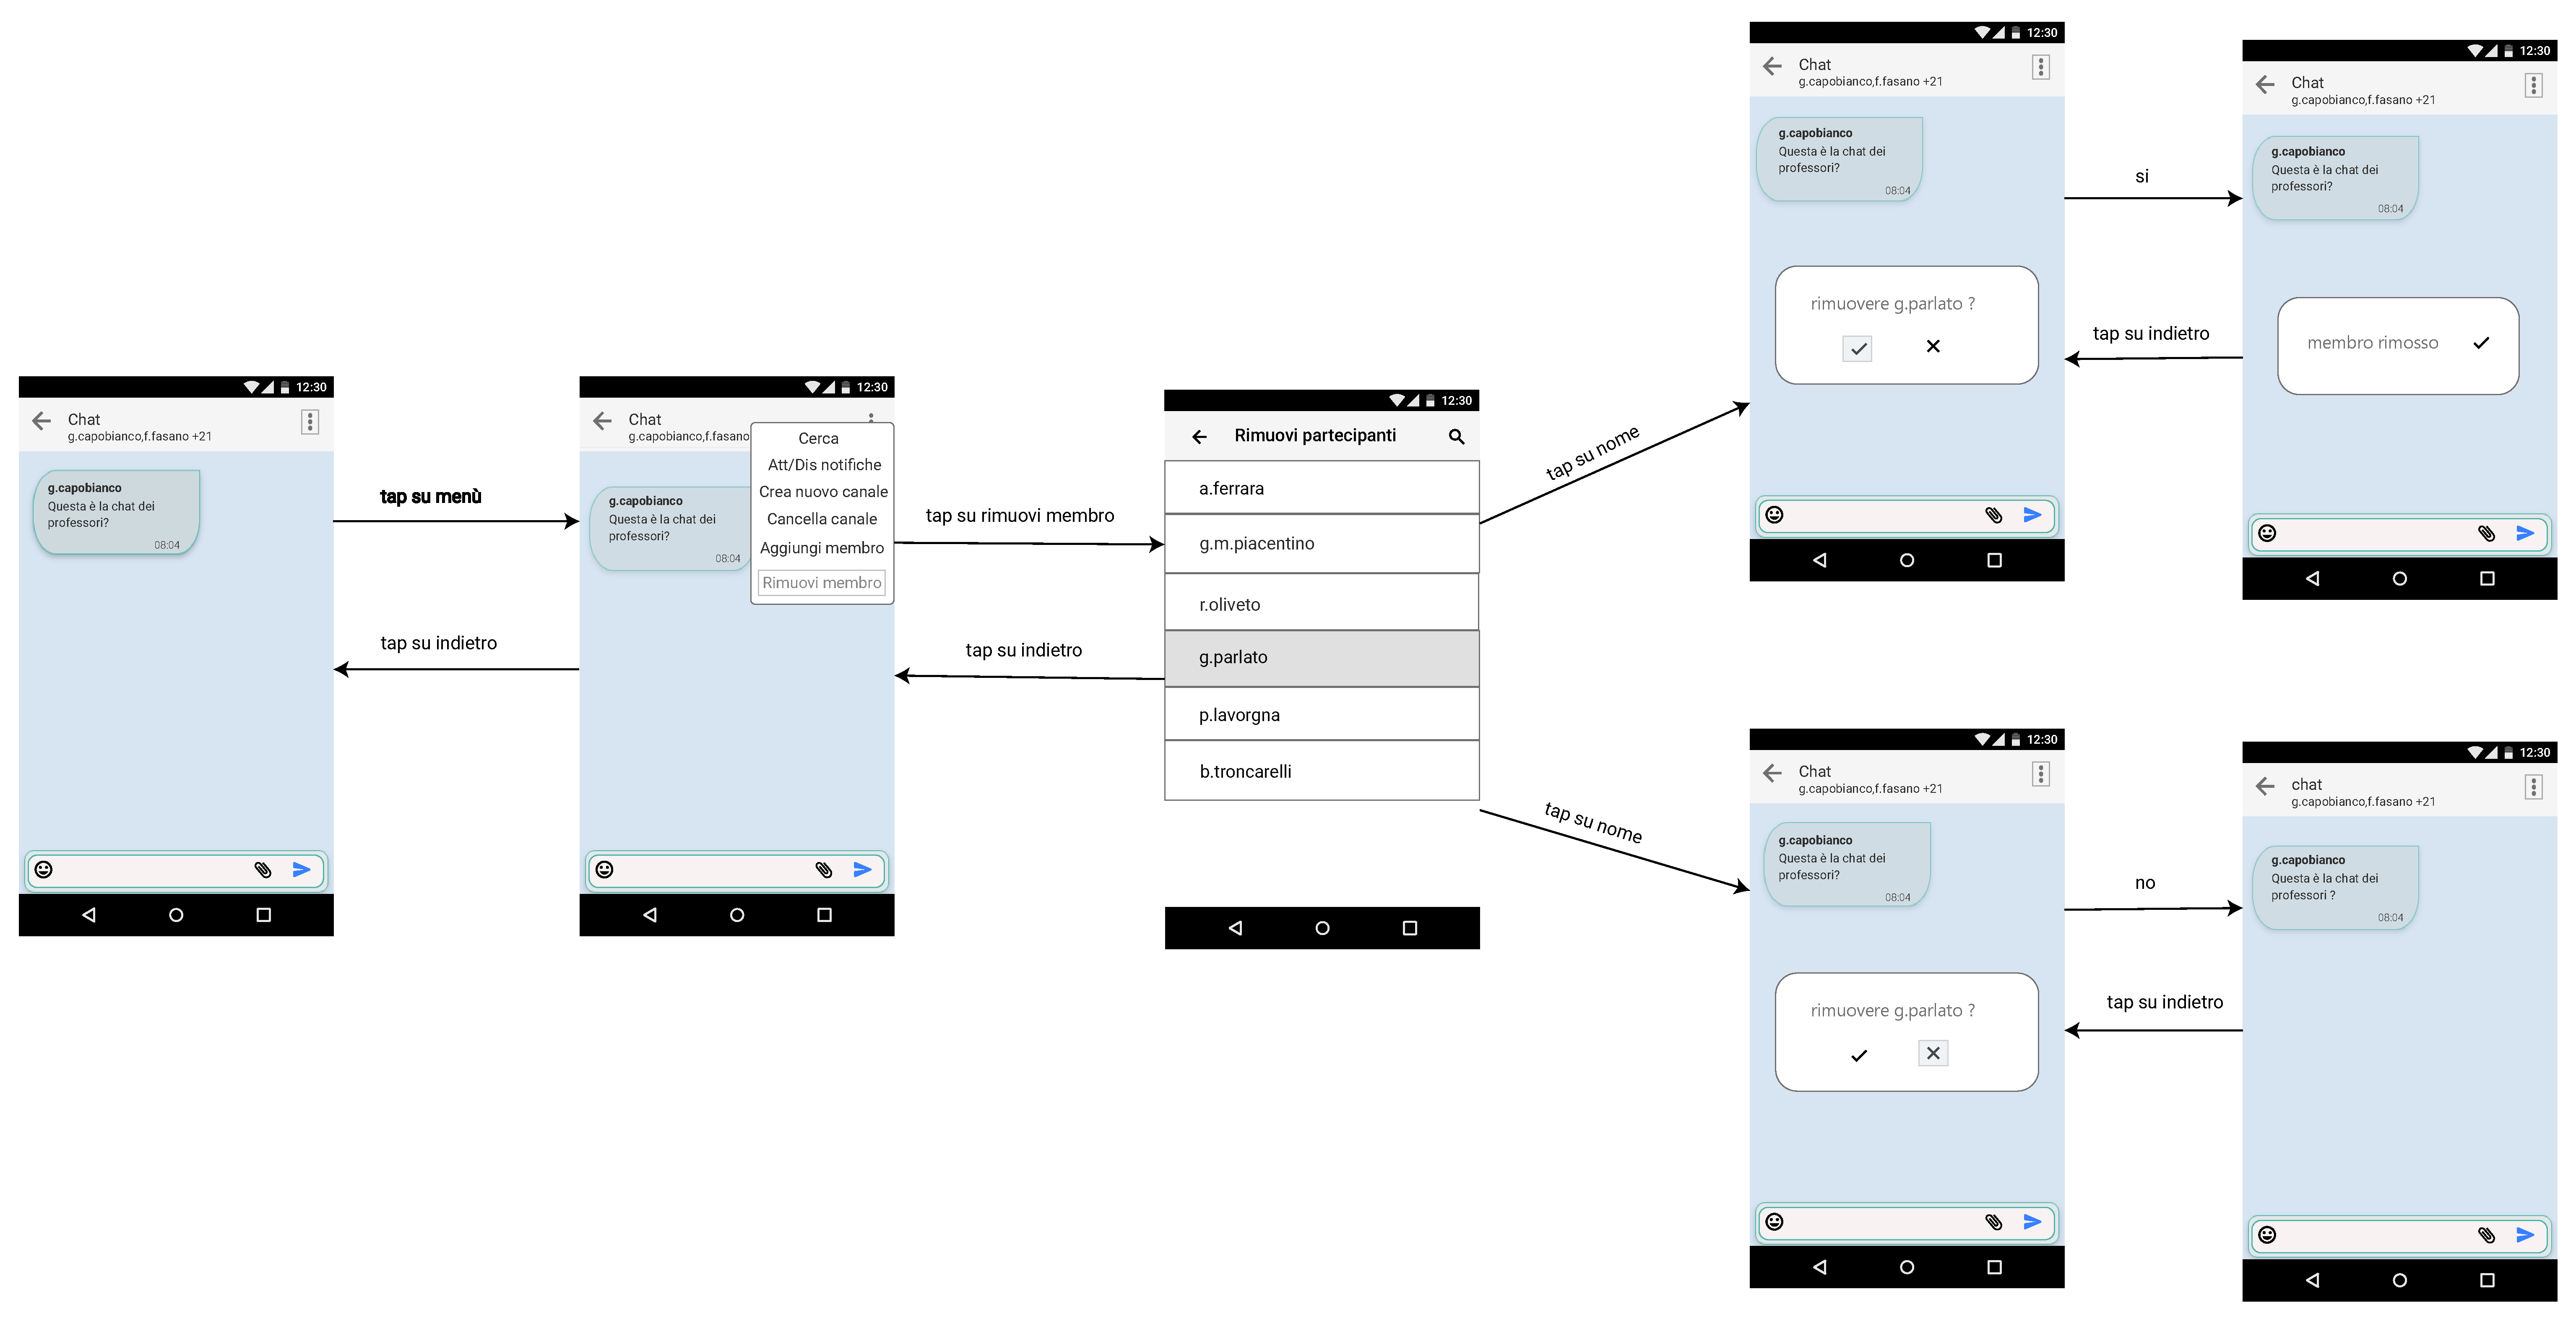
\includegraphics[width=0.9\textwidth]{imgs/gruppo6/activities/act_cud4_rimuovi_membro_da_canale.pdf}
	\caption{CUD4 - Rimuovi membro da un canale}
	\label{fig:cud4}
\end{figure}

\begin{figure}
	\centering
	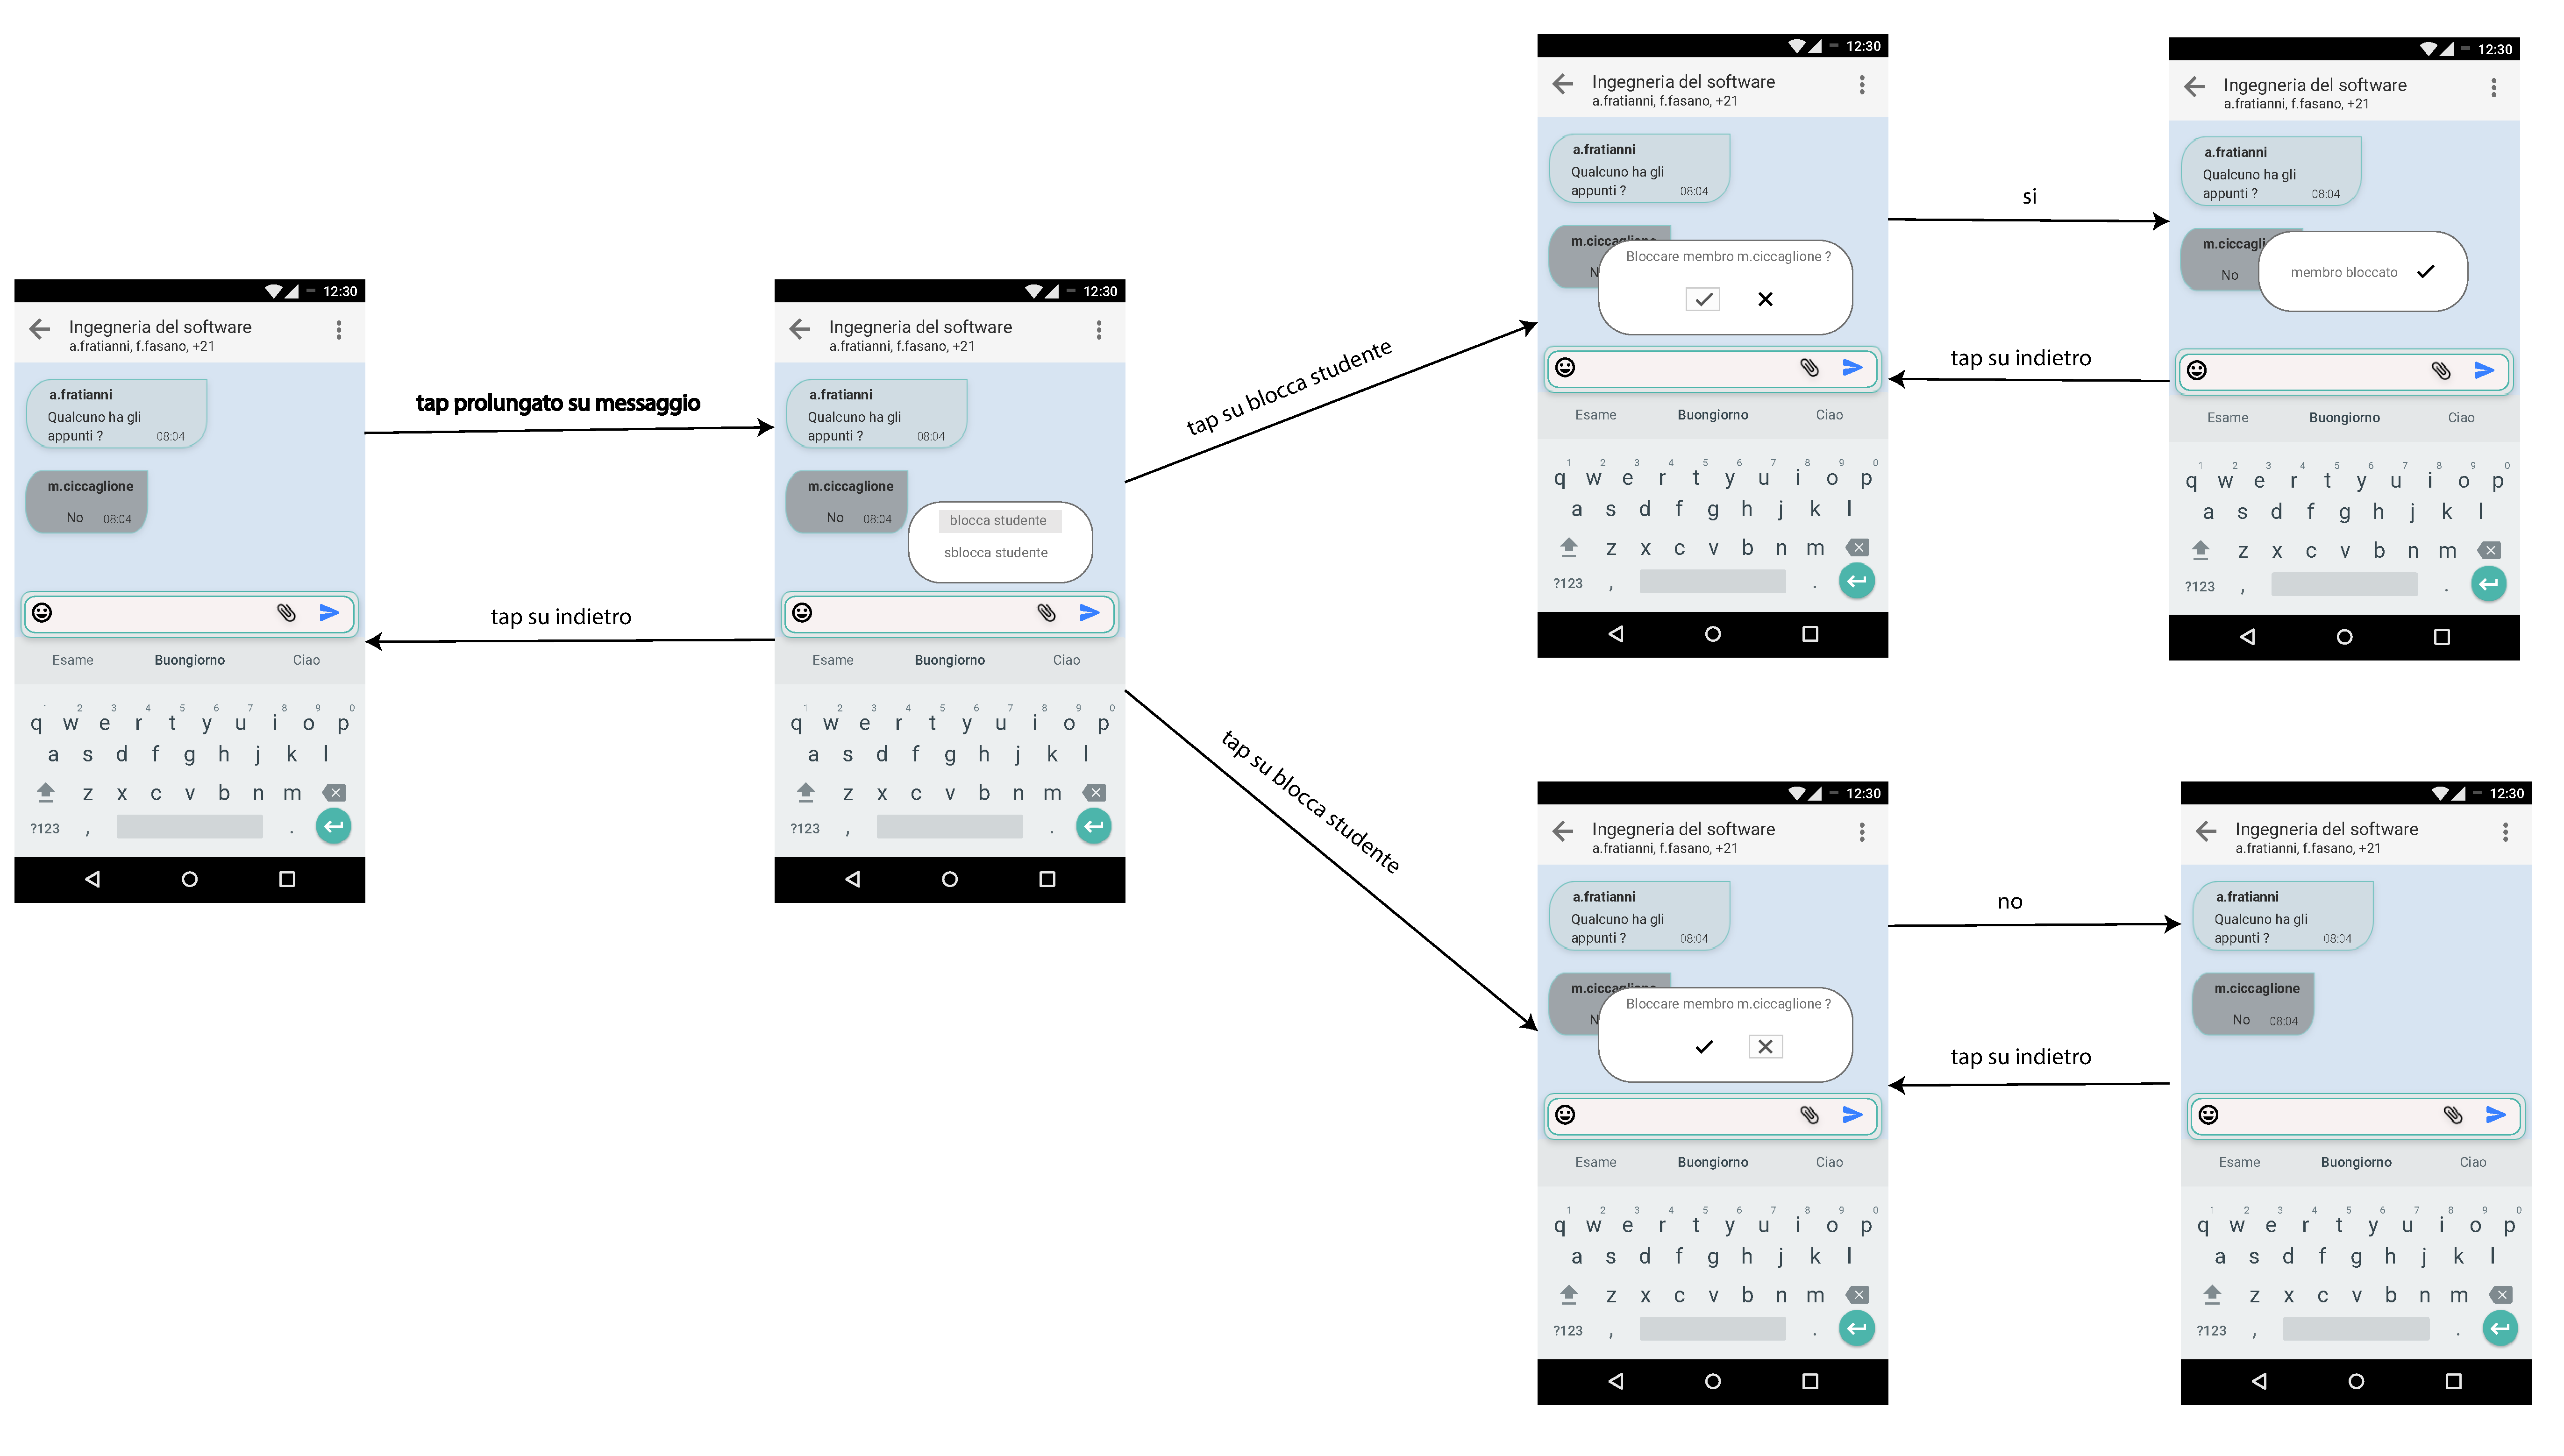
\includegraphics[width=0.9\textwidth]{imgs/gruppo6/activities/act_cud5_blocca_studente.pdf}
	\caption{CUD5 - Blocca Studente}
	\label{fig:cud5}
\end{figure}

\begin{figure}
	\centering
	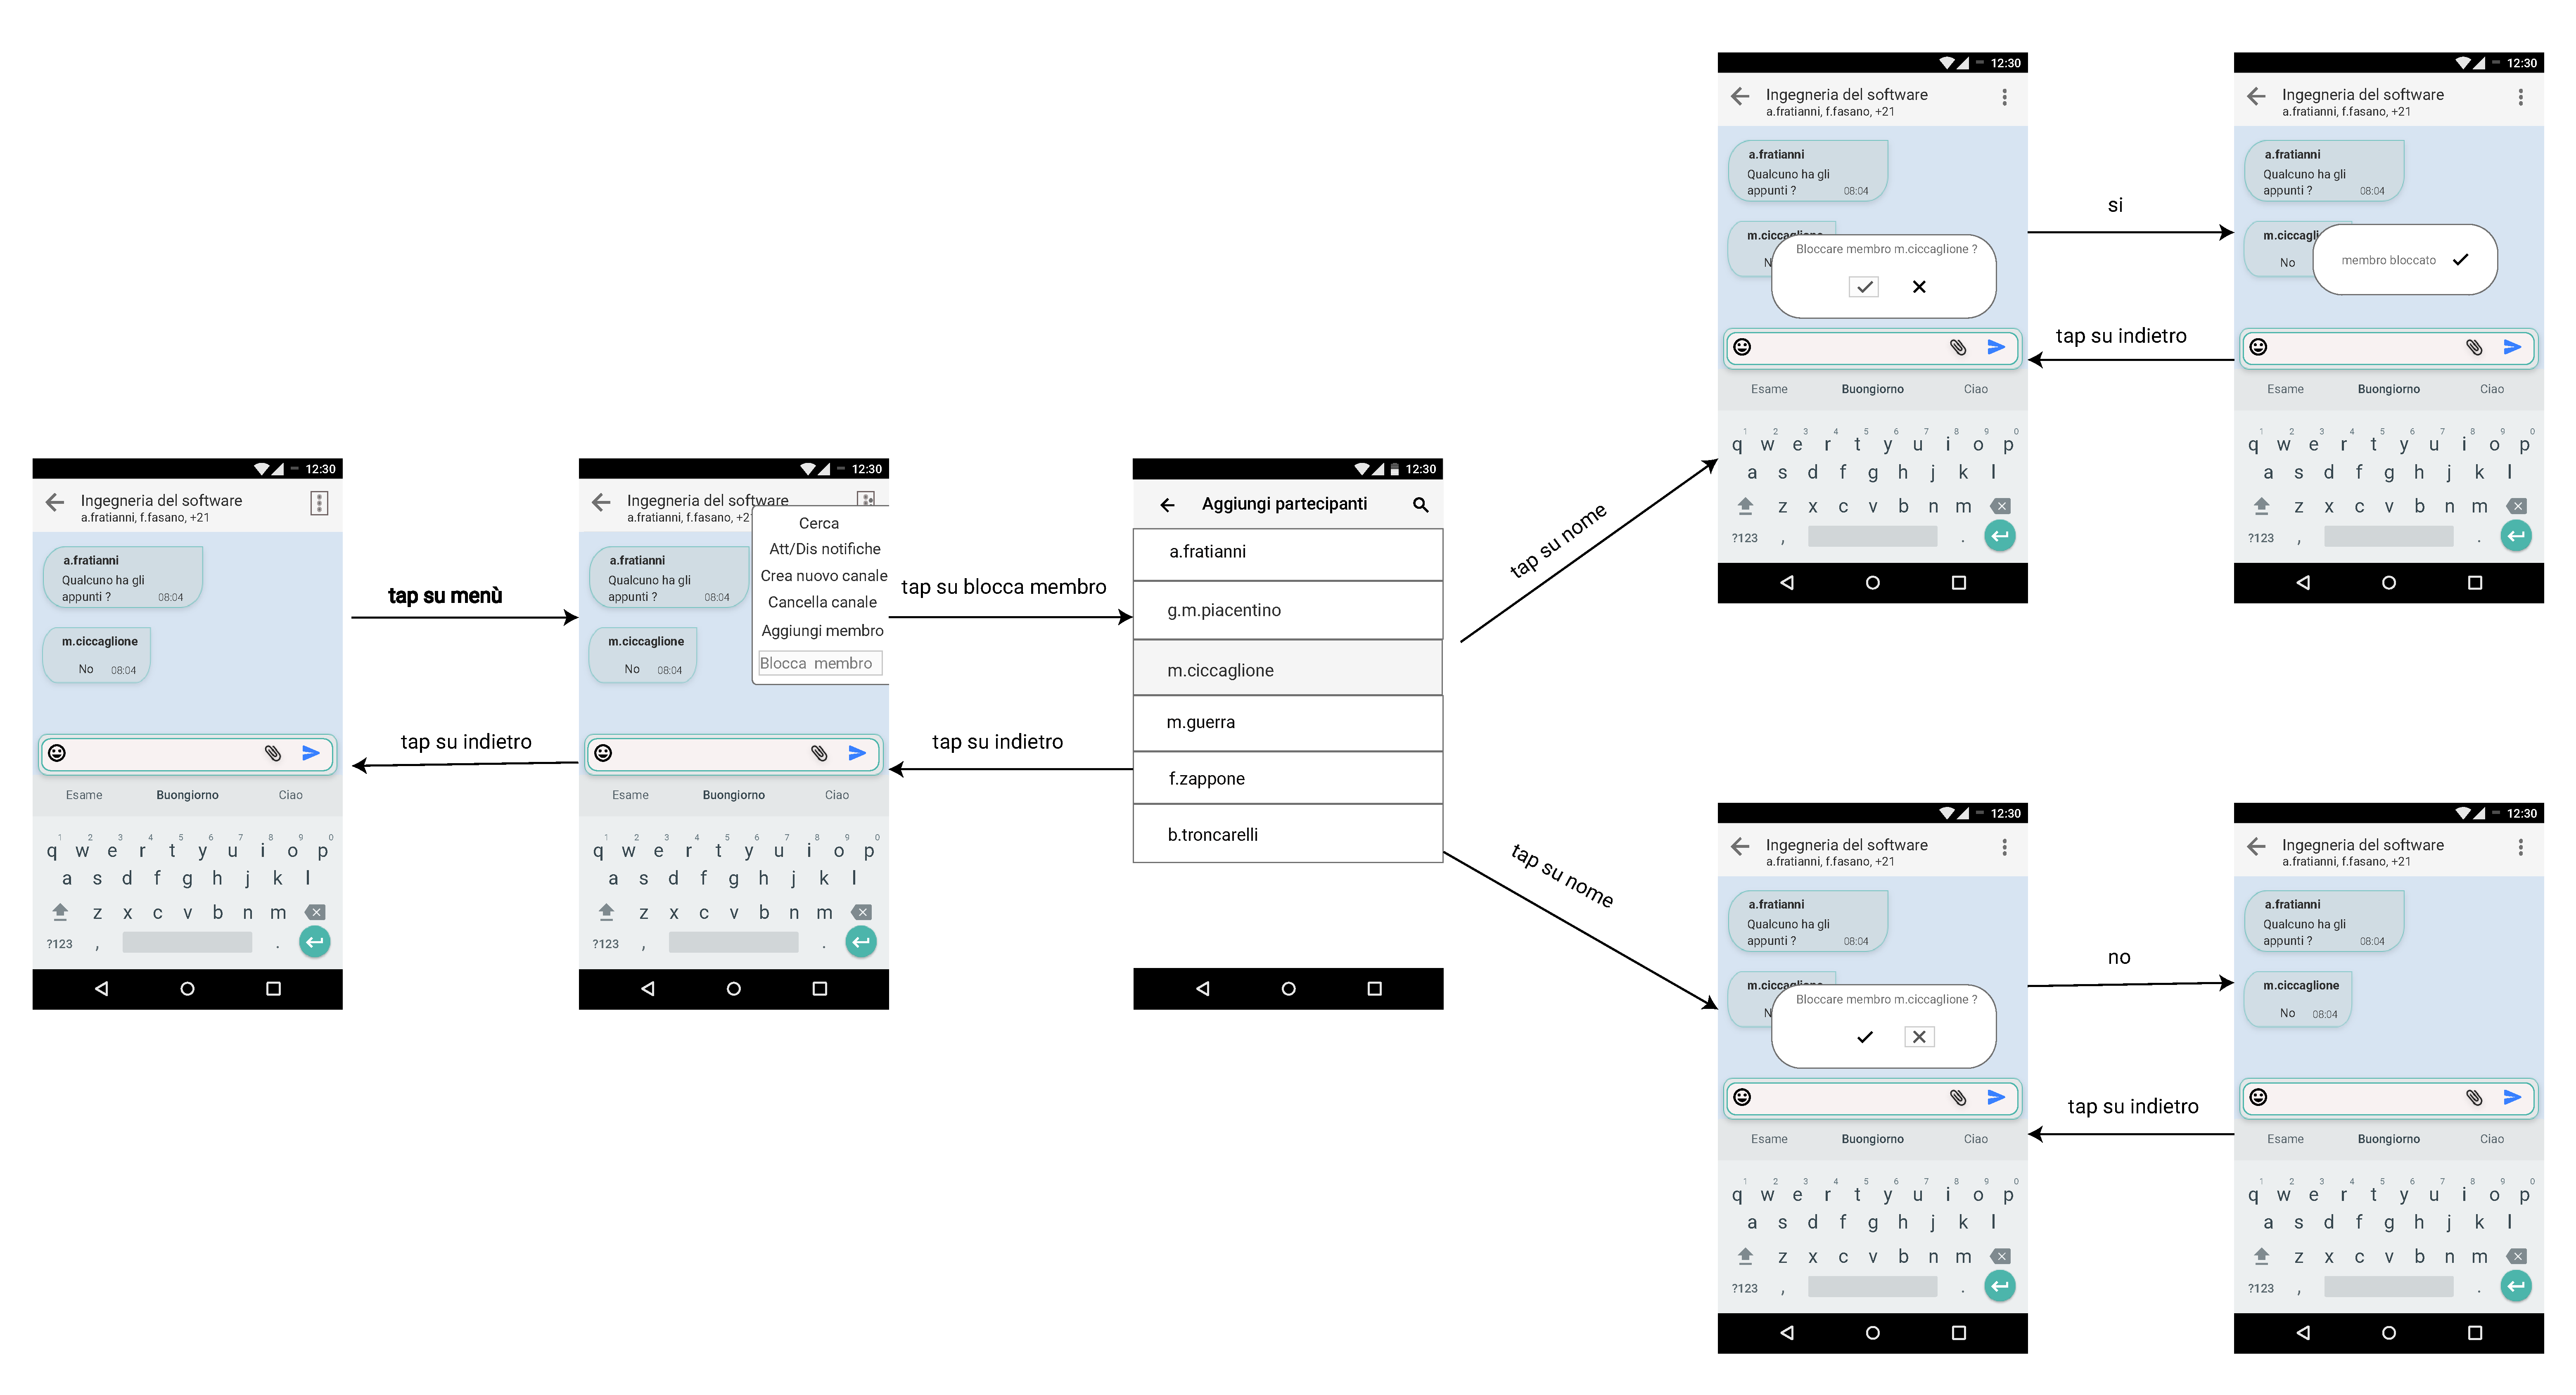
\includegraphics[width=0.9\textwidth]{imgs/gruppo6/activities/act_cud5_blocca_studente2.pdf}
	\caption{CUD5 - Blocca Studente (es. 2}
	\label{fig:cud5-2}
\end{figure}

\begin{figure}
	\centering
	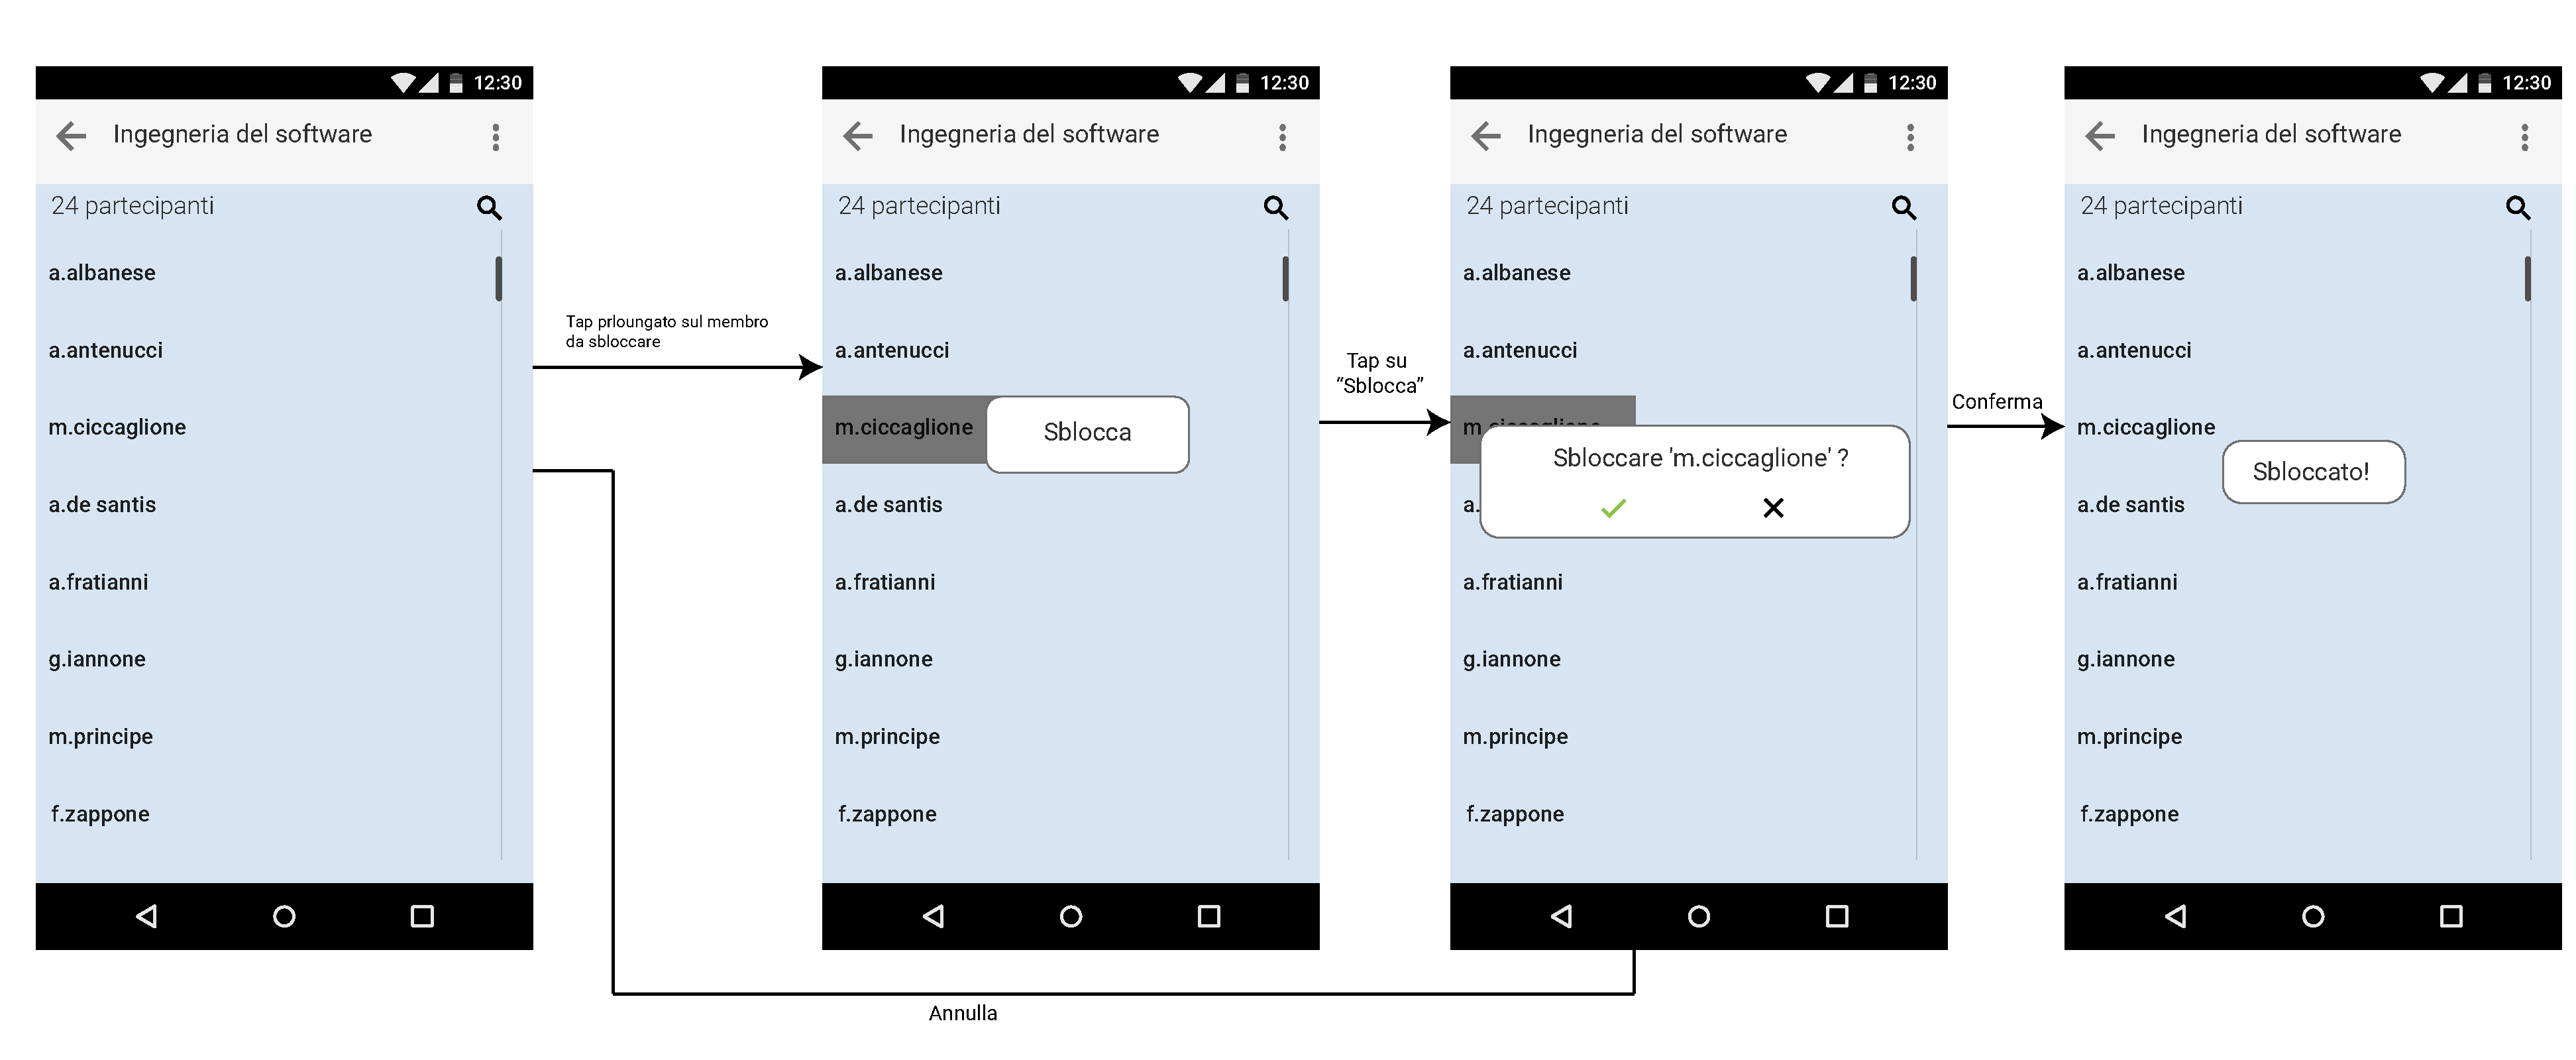
\includegraphics[width=0.9\textwidth]{imgs/gruppo6/activities/act_cud6_sblocca_da_elenco.pdf}
	\caption{CUD6 - Sblocca Studente (da elenco)}
	\label{fig:cud6}
\end{figure}

\begin{figure}
	\centering
	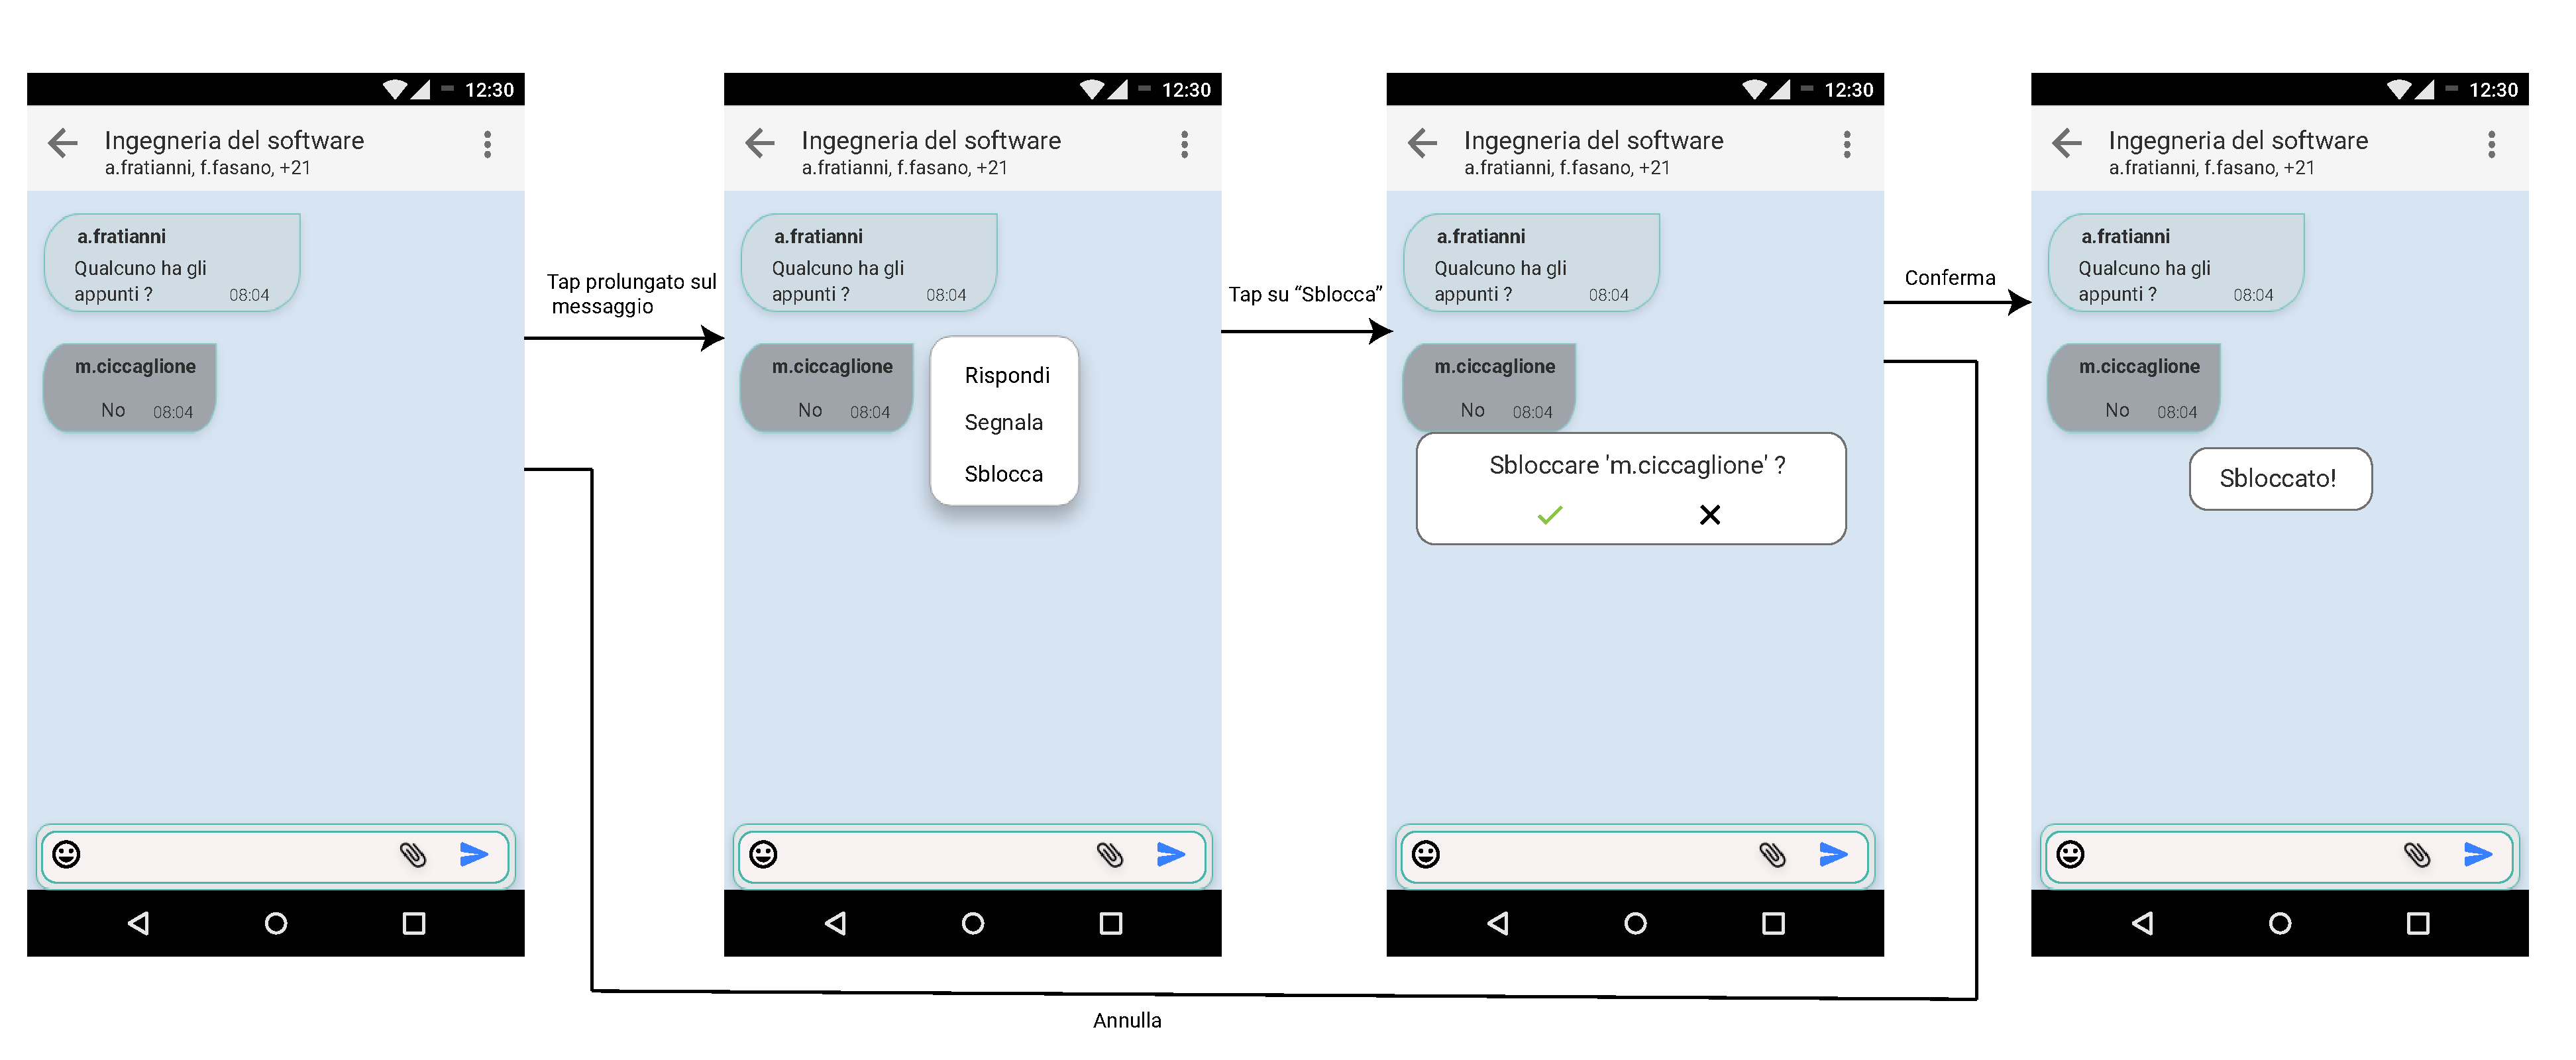
\includegraphics[width=0.9\textwidth]{imgs/gruppo6/activities/act_cud6_sblocca_da_messaggio.pdf}
	\caption{CUD6 - Sblocca Studente (da messaggio)}
	\label{fig:cud6}
\end{figure}
%%% END activities chat docenti %%%

%%% START activities chat pannello %%%
\pagebreak
\begin{figure}
\subsection{Activities relative al pannello di amministrazione}
	\centering
	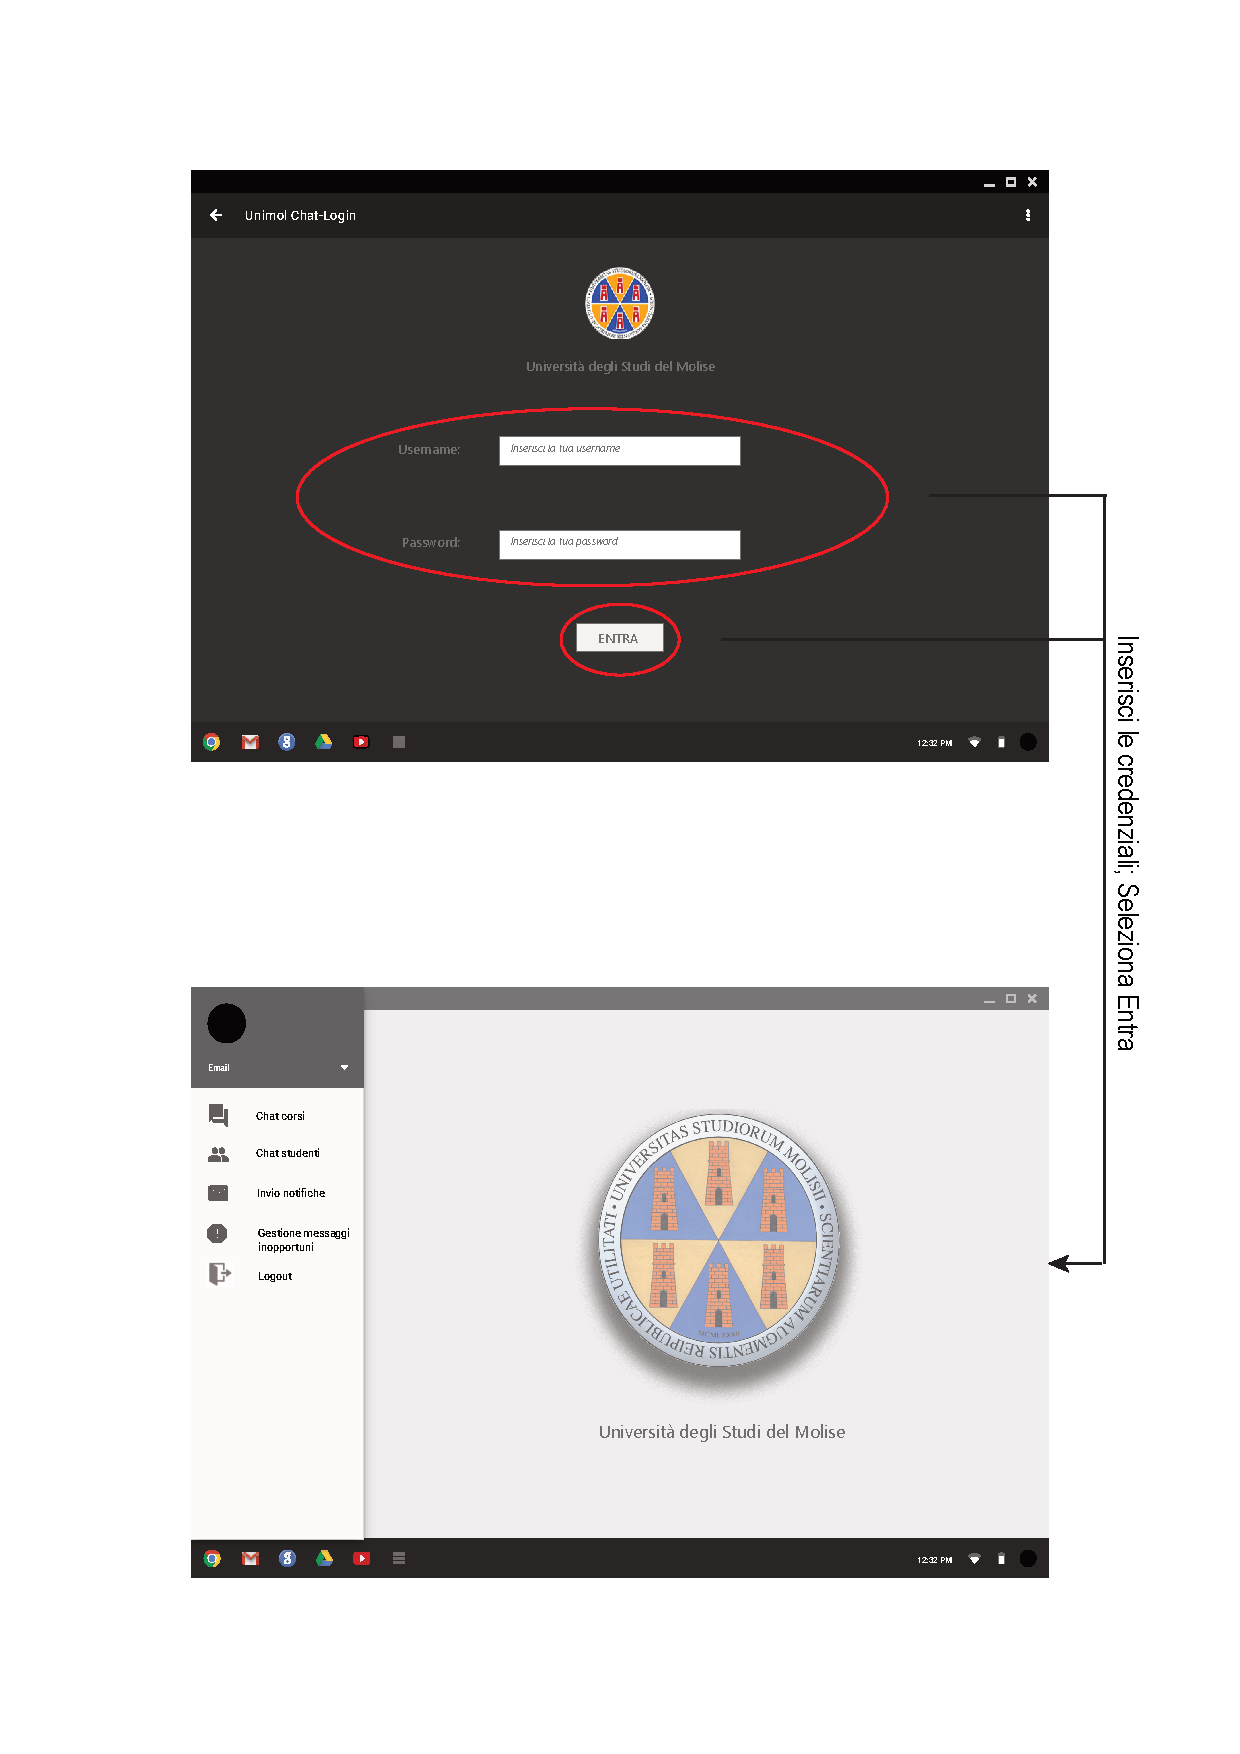
\includegraphics[width=0.9\textwidth]{imgs/gruppo6/activities/act_cup1_login.pdf}
	\caption{CUP1 - Login}
	\label{fig:cup1}
\end{figure}

\begin{figure}
	\centering
	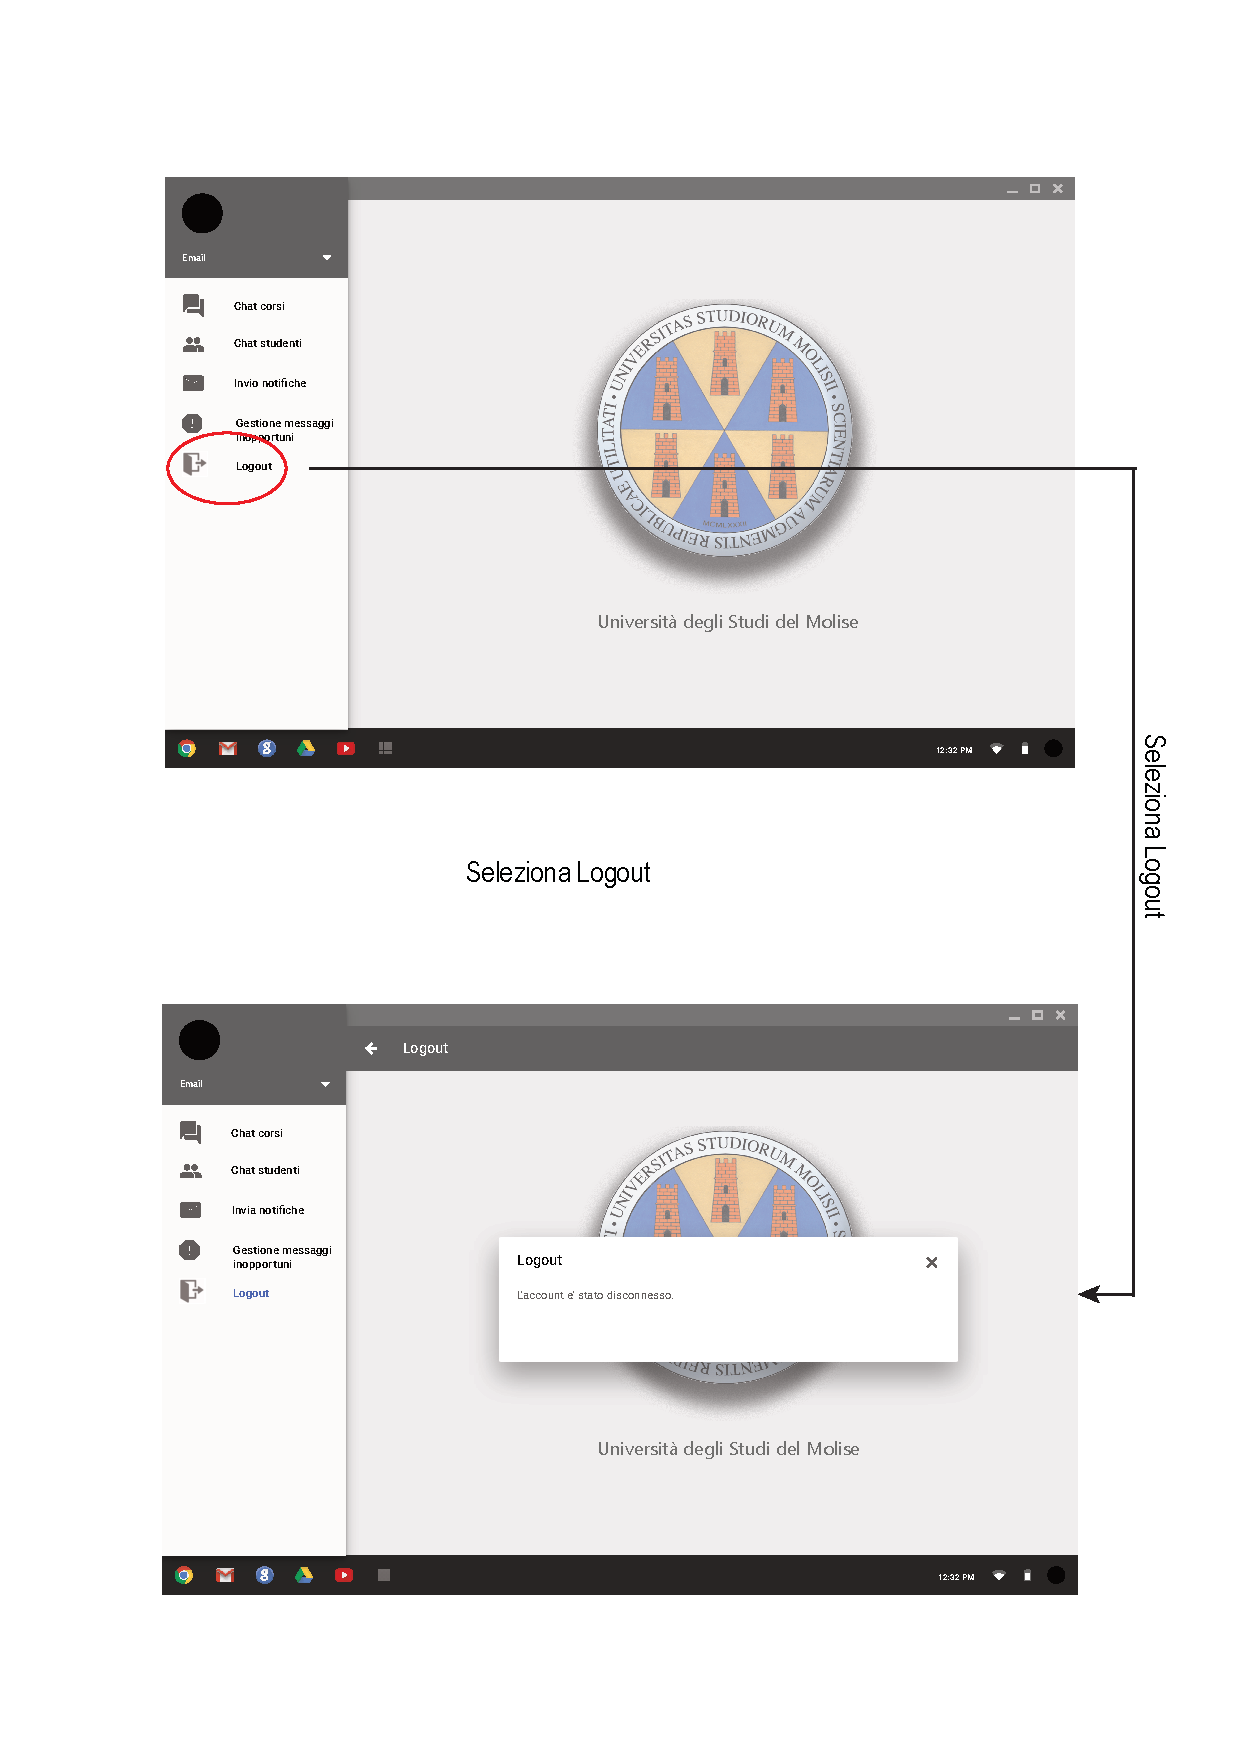
\includegraphics[width=0.9\textwidth]{imgs/gruppo6/activities/act_cup2_logout.pdf}
	\caption{CUP2 - Logout}
	\label{fig:cup2}
\end{figure}

\begin{figure}
	\centering
	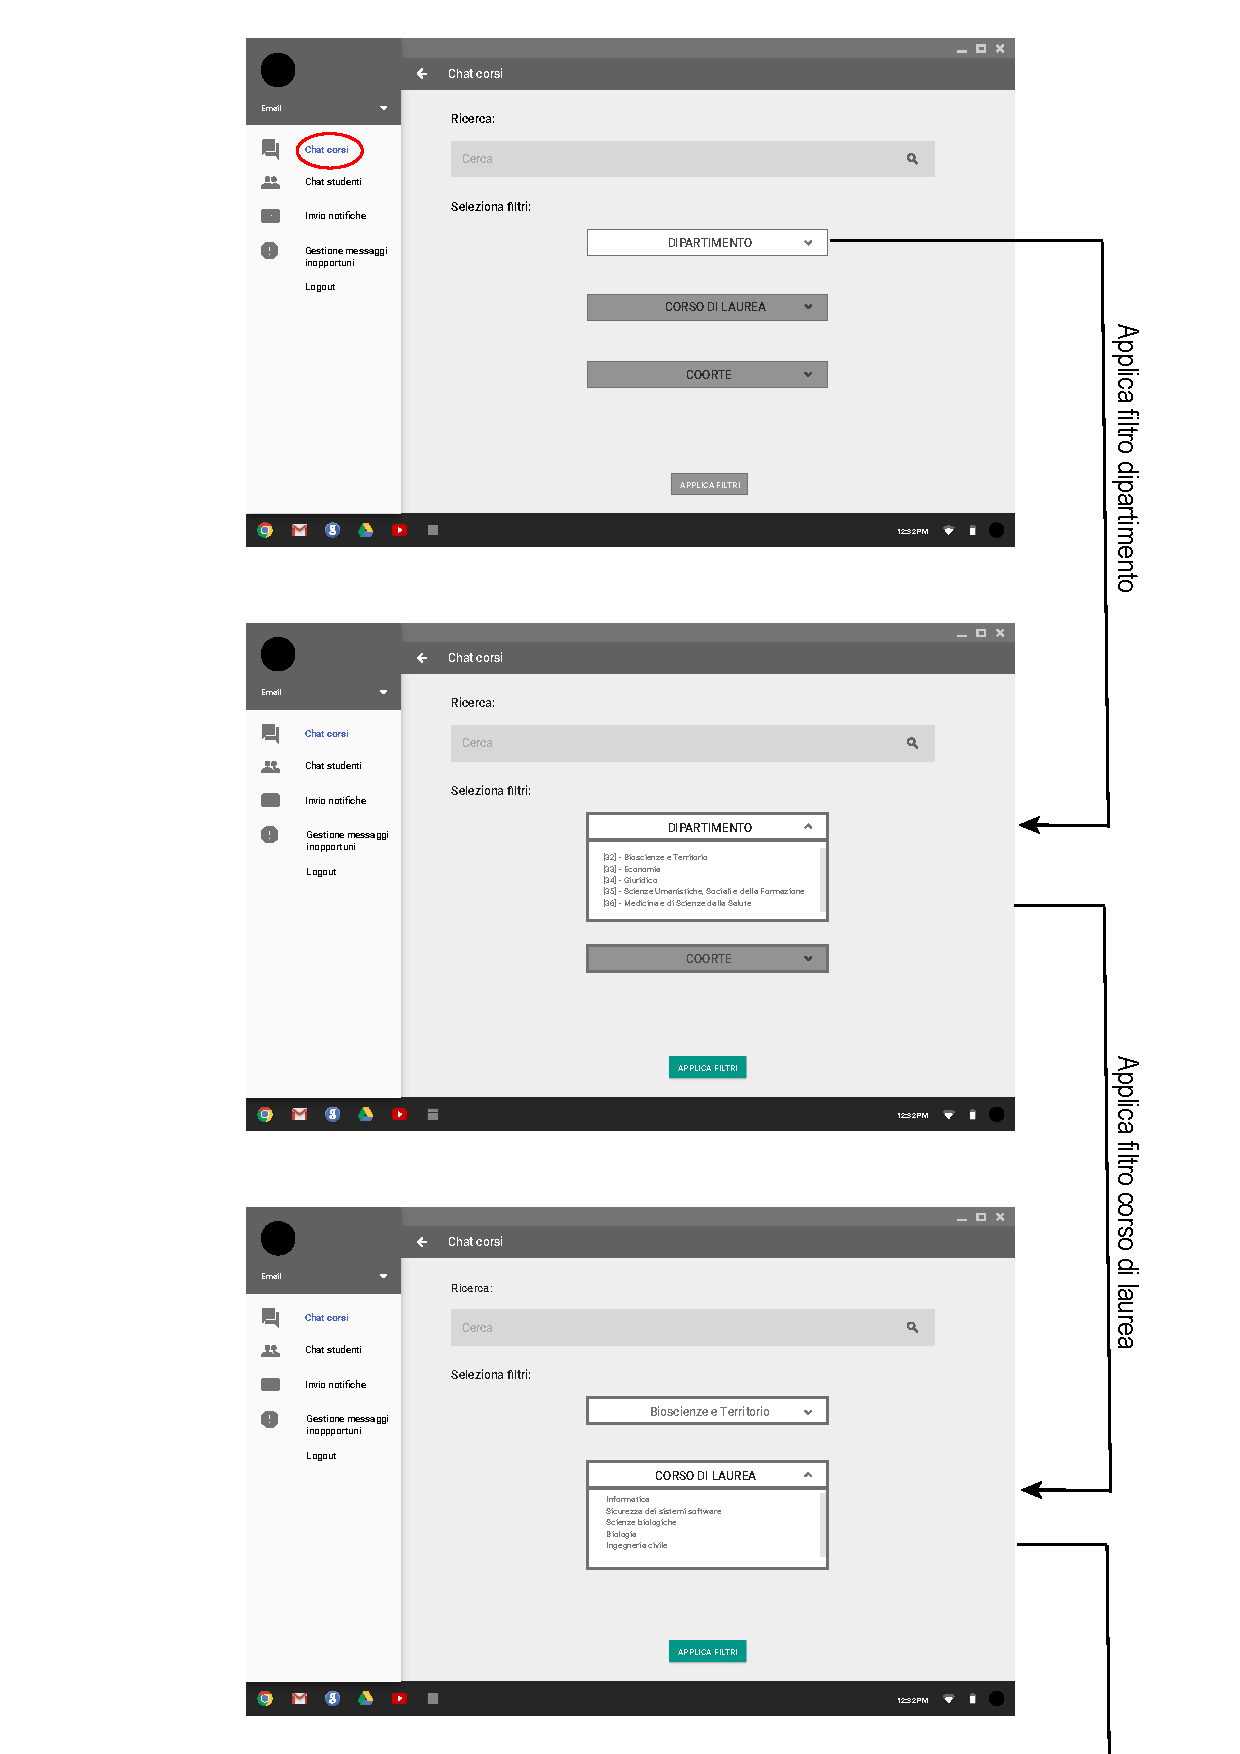
\includegraphics[width=0.9\textwidth]{imgs/gruppo6/activities/act_cup3_filtro_chat_corsi1.pdf}
	\caption{CUP3 - Ricerca chat (filtri chat corsi - pt.1)}
	\label{fig:cup3}
\end{figure}

\begin{figure}
	\centering
	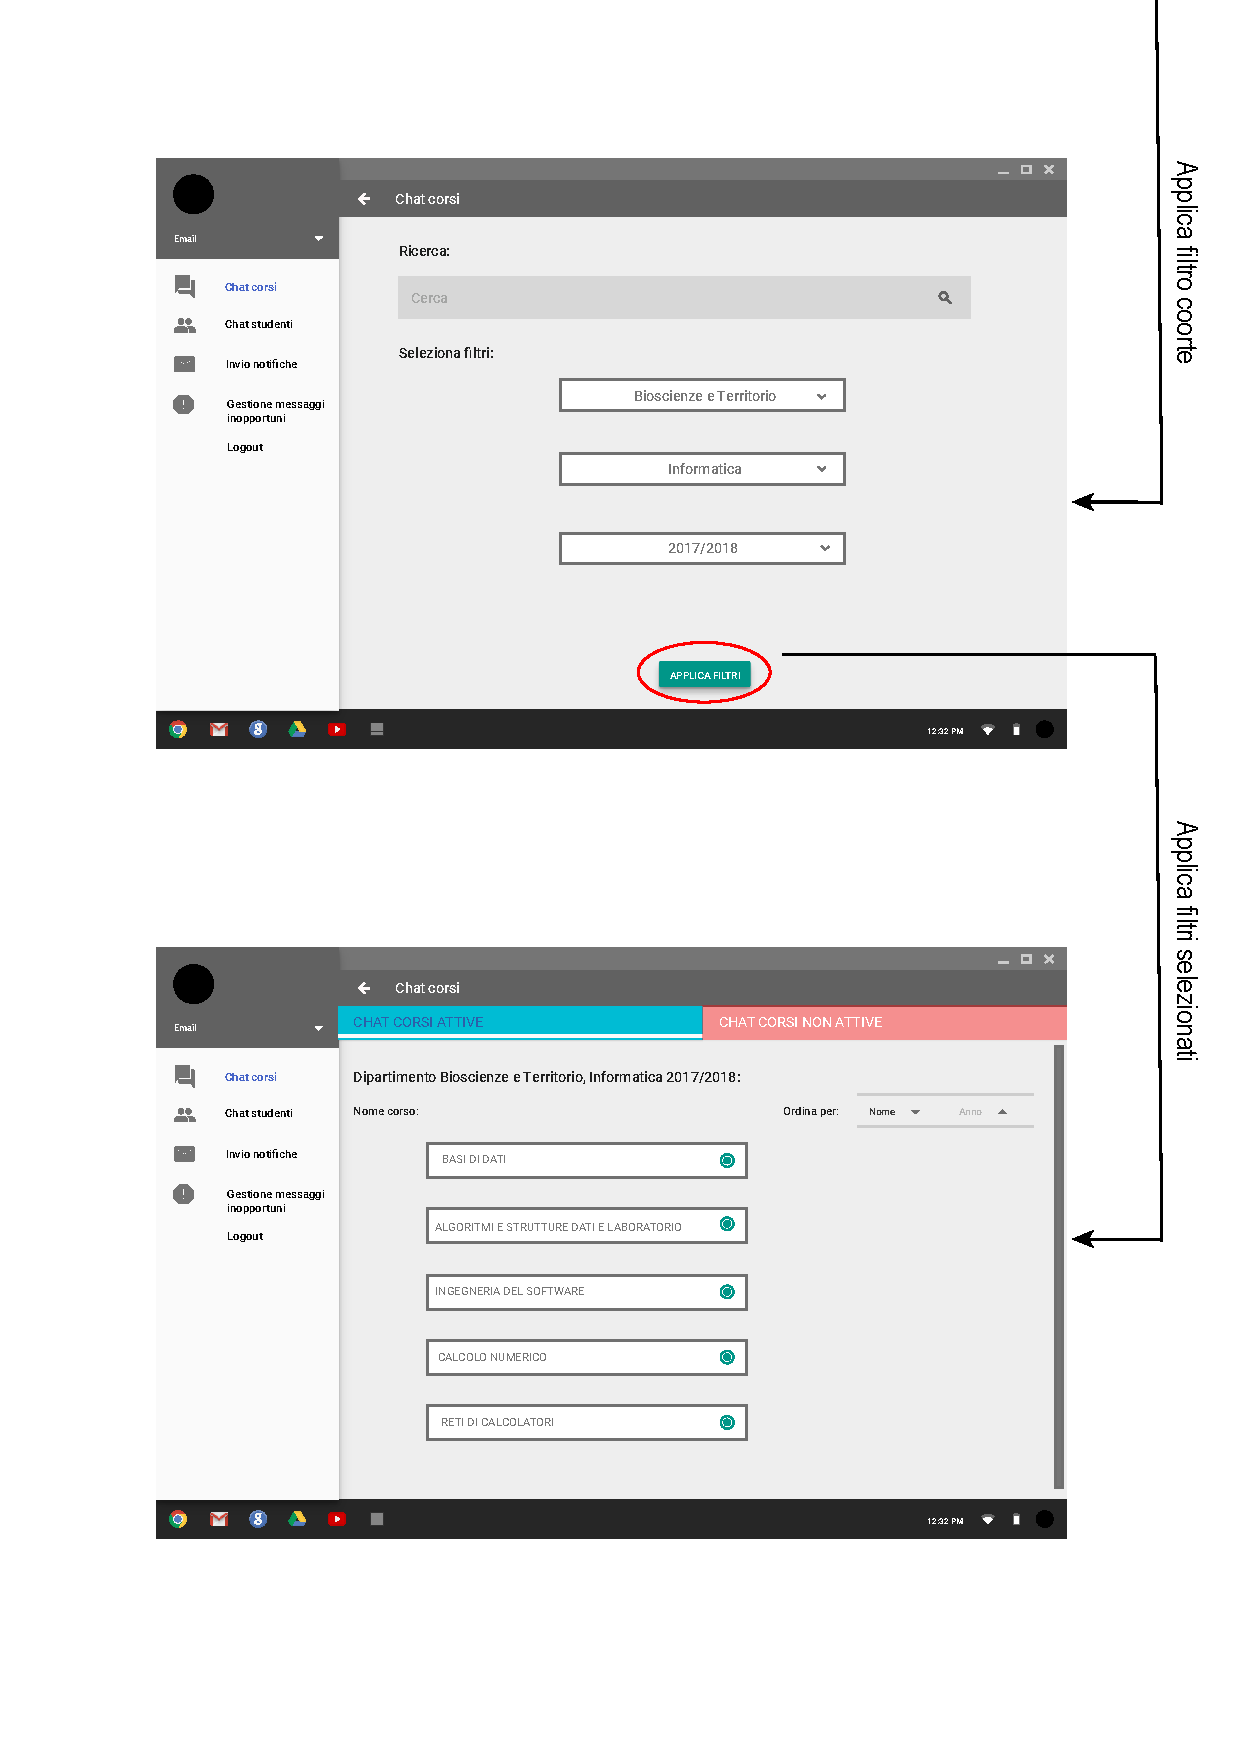
\includegraphics[width=0.9\textwidth]{imgs/gruppo6/activities/act_cup3_filtro_chat_corsi2.pdf}
	\caption{CUP3 - Ricerca chat (filtri chat corsi - pt.2)}
	\label{fig:cup3-2}
\end{figure}

\begin{figure}
	\centering
	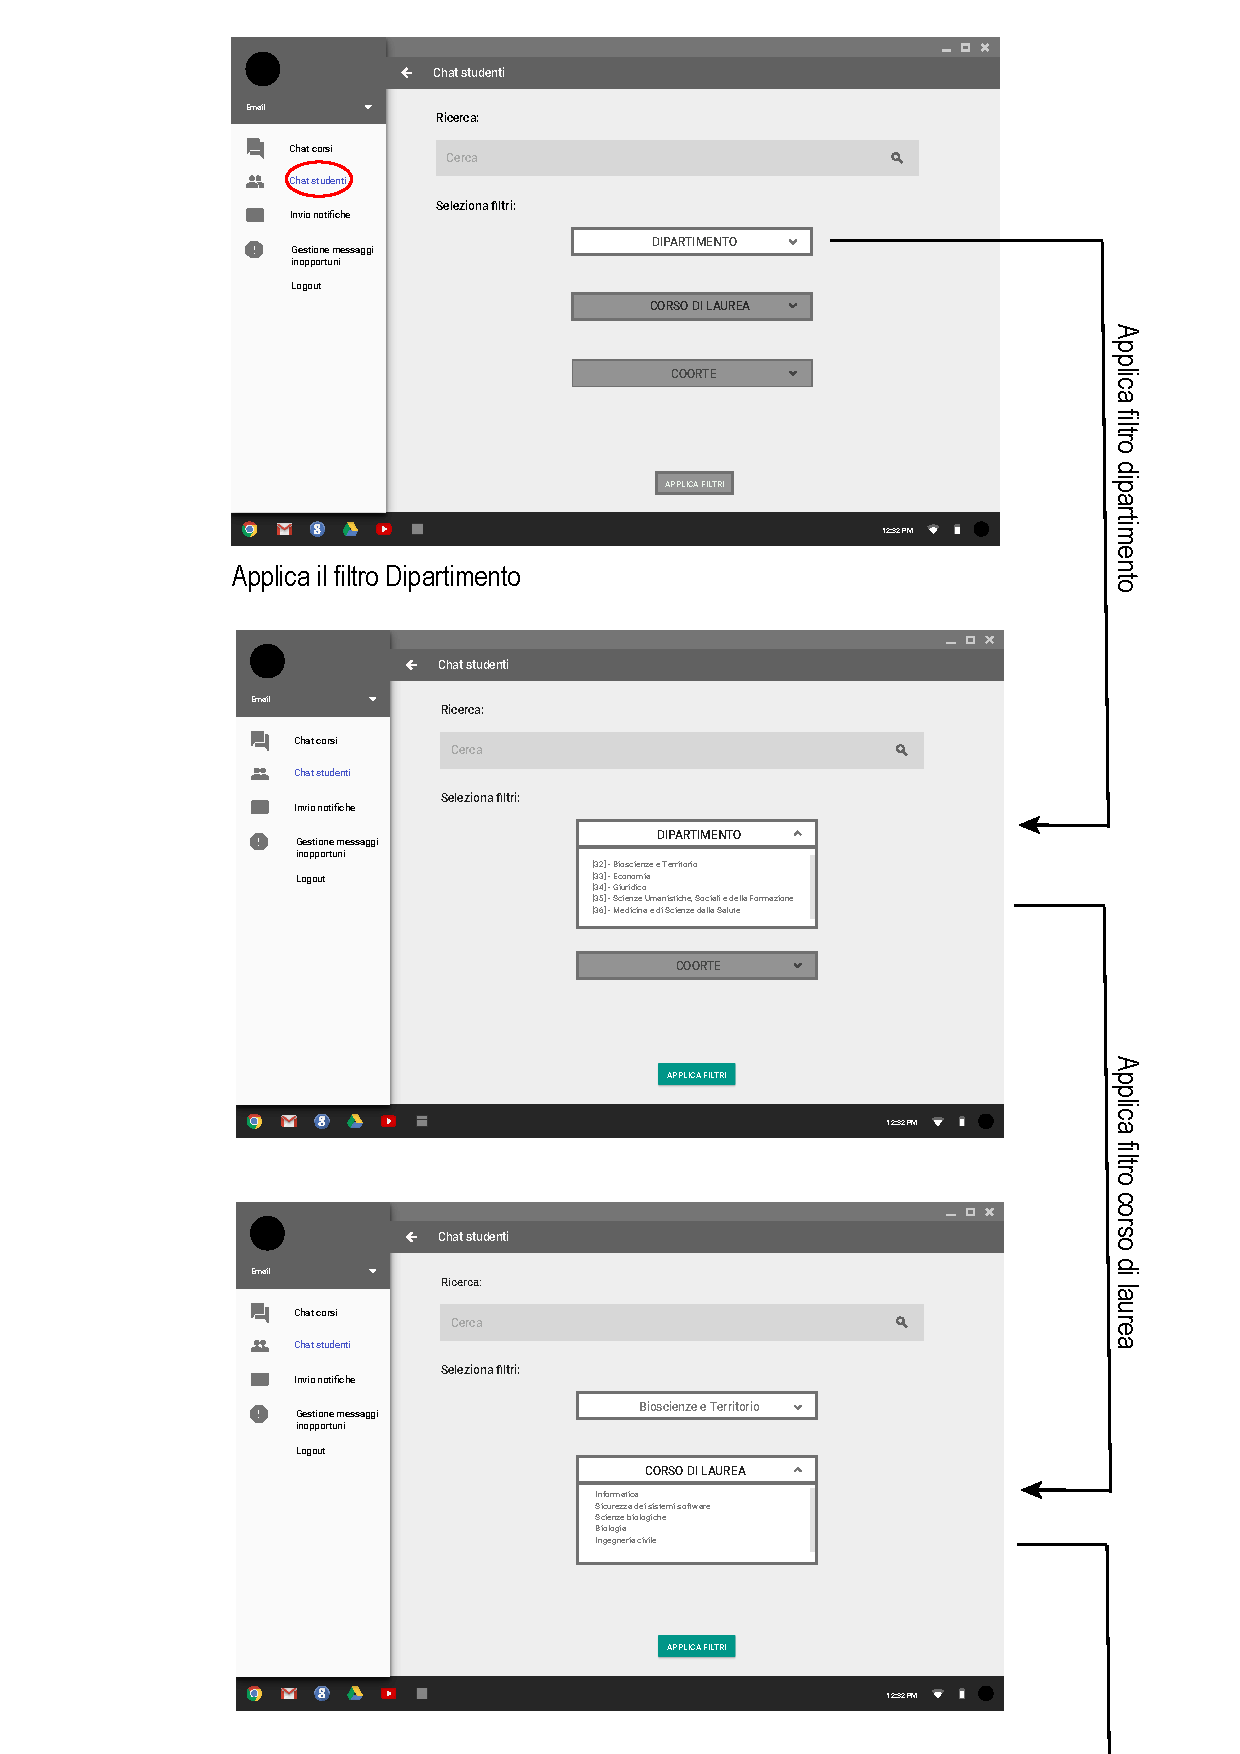
\includegraphics[width=0.9\textwidth]{imgs/gruppo6/activities/act_cup3_filtro_chat_studenti1.pdf}
	\caption{CUP3 - Ricerca chat (filtri chat studenti - pt.1)}
	\label{fig:cup3-3}
\end{figure}

\begin{figure}
	\centering
	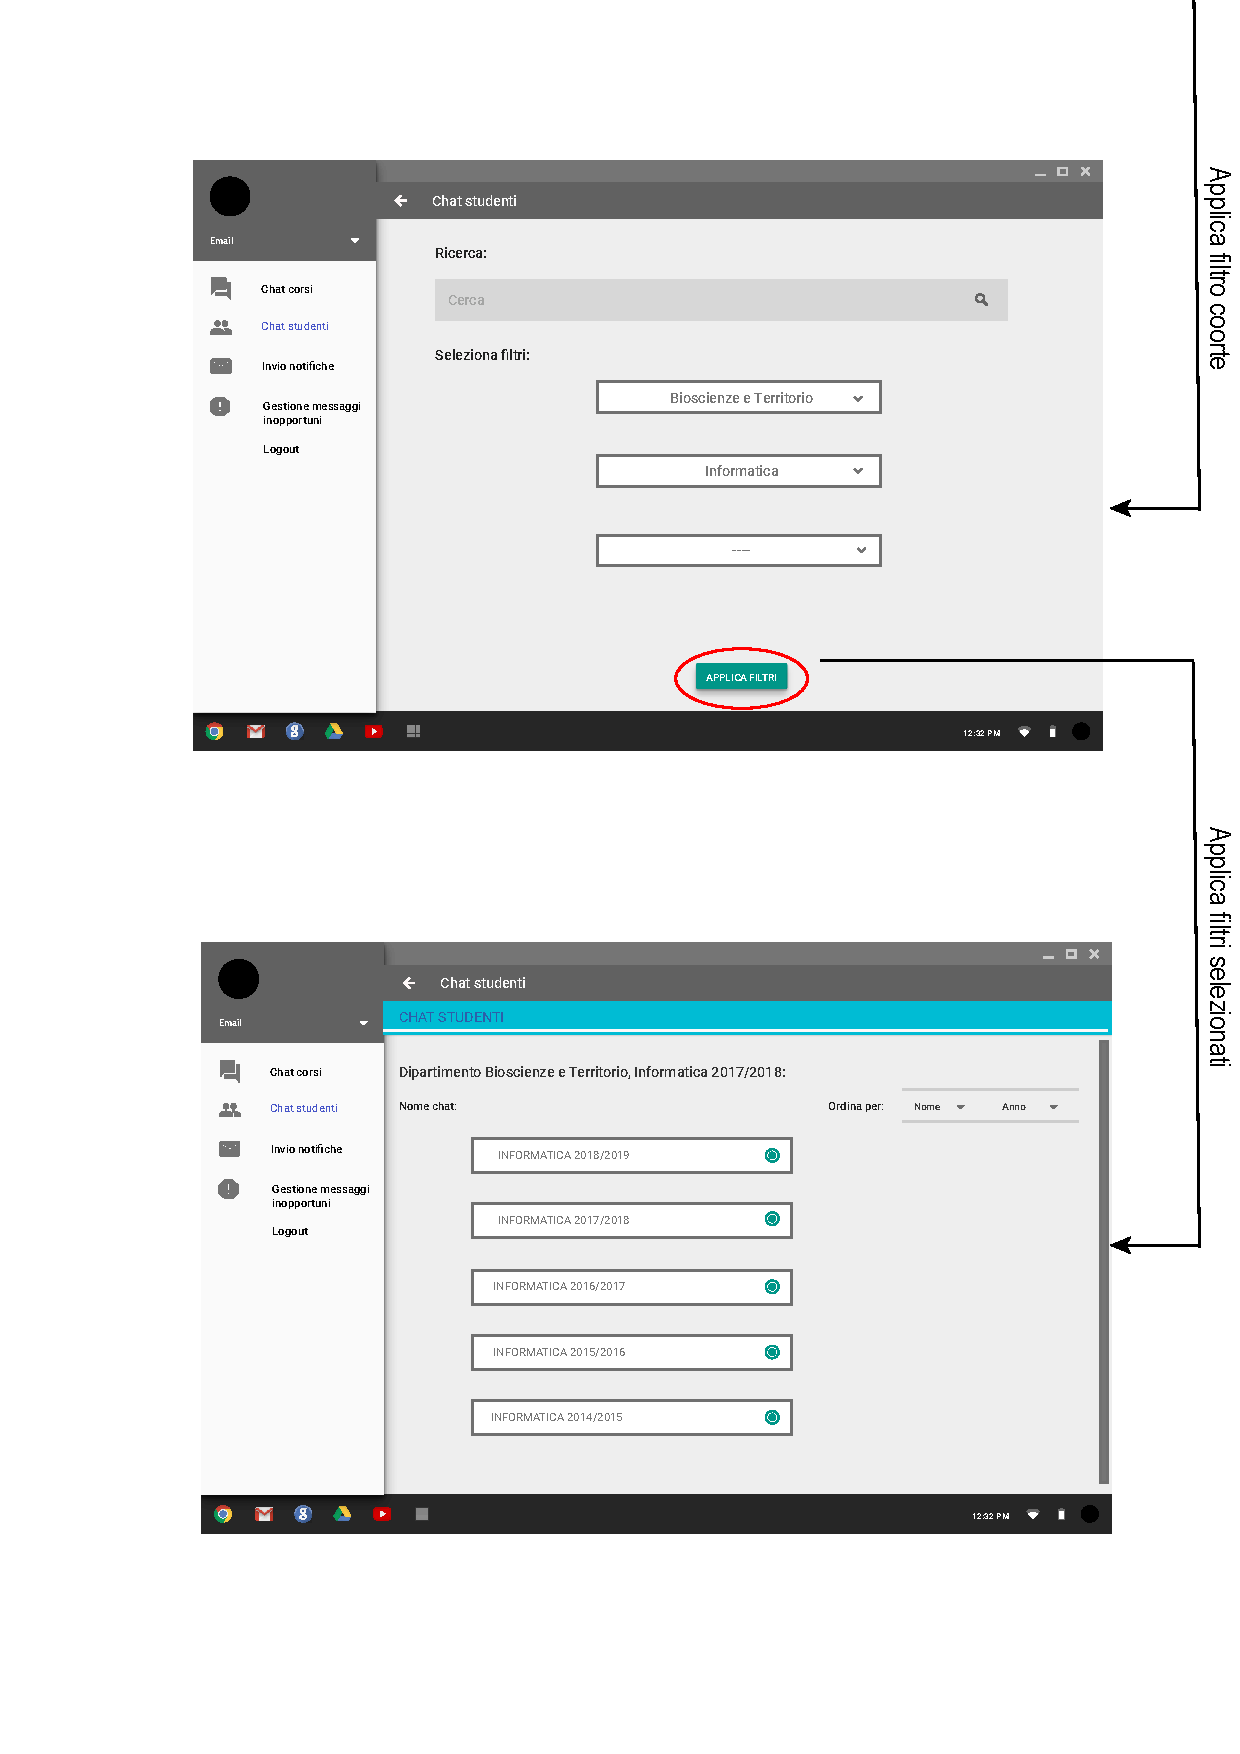
\includegraphics[width=0.9\textwidth]{imgs/gruppo6/activities/act_cup3_filtro_chat_studenti2.pdf}
	\caption{CUP3 - Ricerca chat (filtri chat studenti - pt.2)}
	\label{fig:cup3-4}
\end{figure}

\begin{figure}
	\centering
	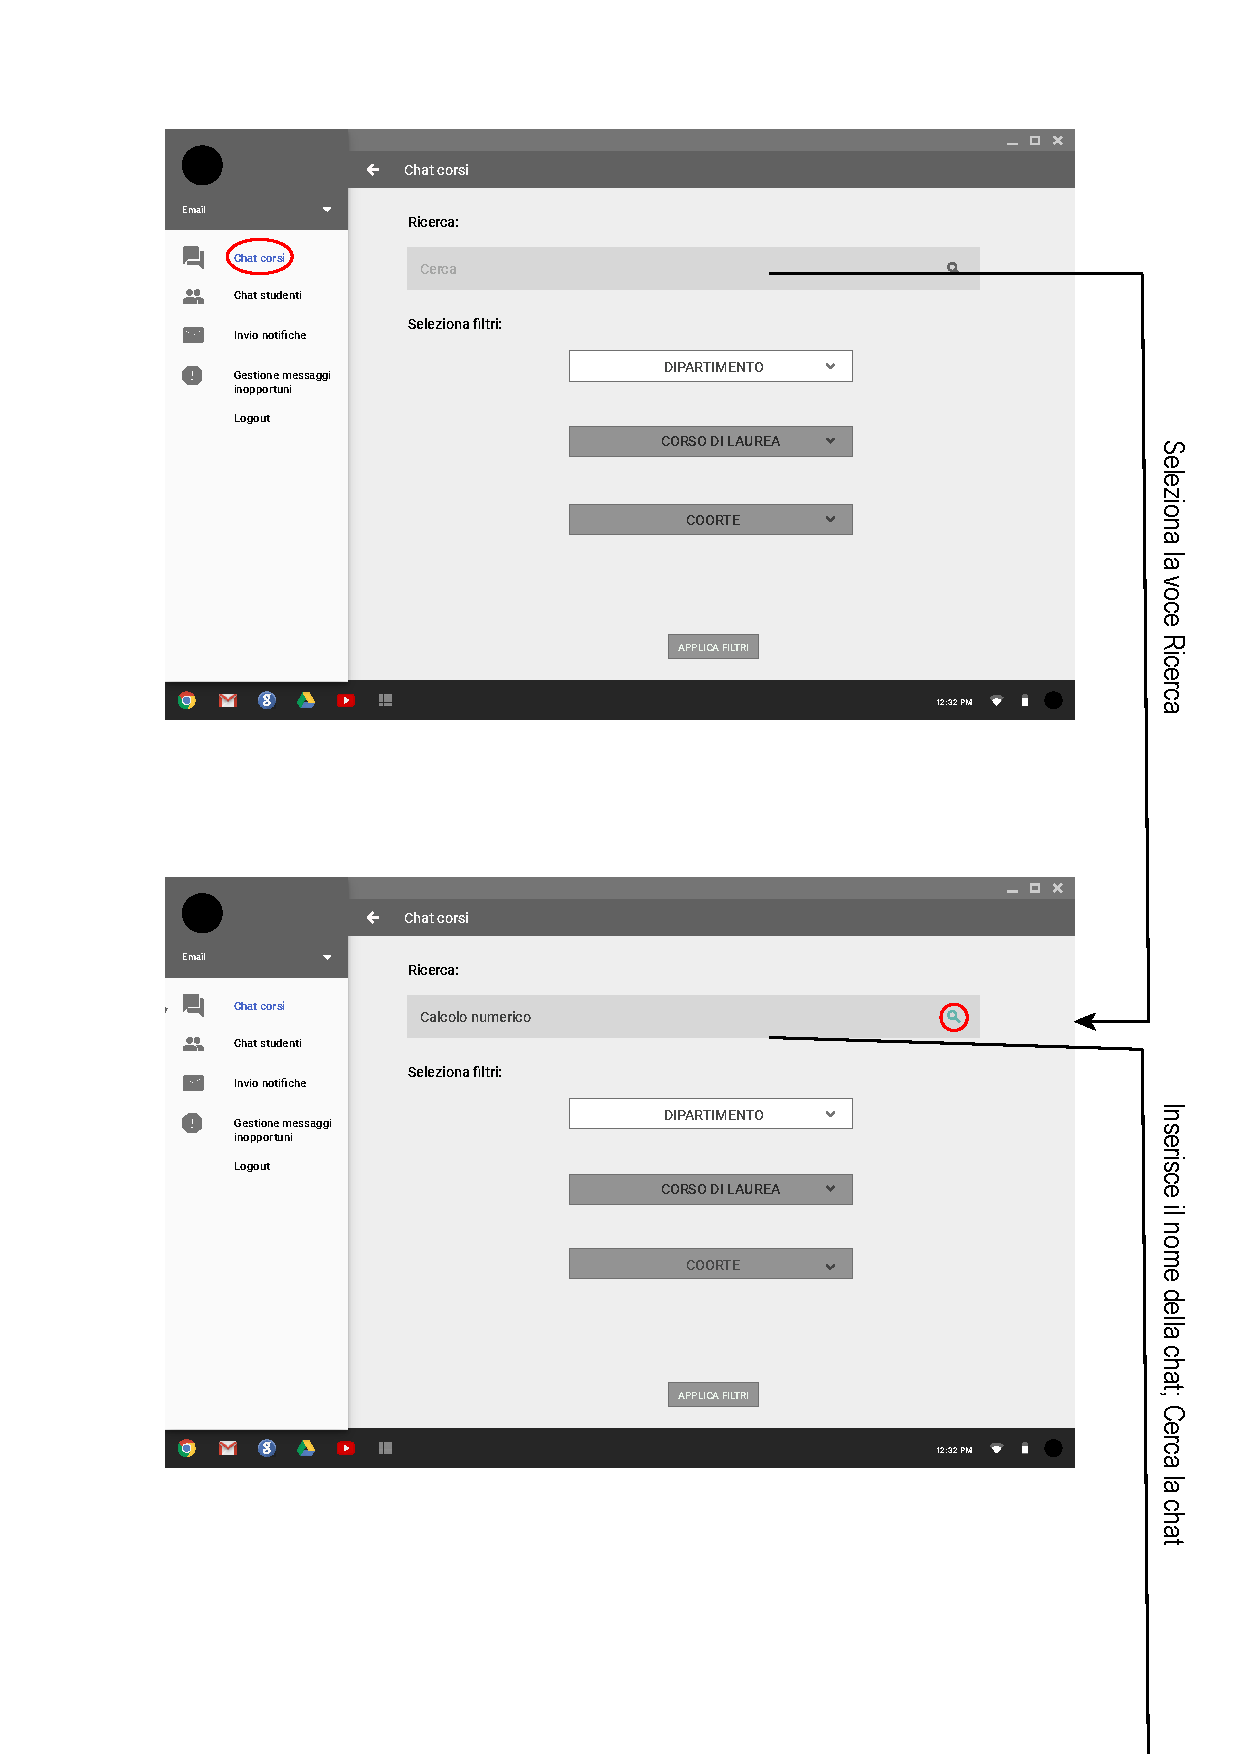
\includegraphics[width=0.9\textwidth]{imgs/gruppo6/activities/act_cup3_ricerca_chat_corsi1.pdf}
	\caption{CUP3 - Ricerca chat (cerca corsi - pt.1)}
	\label{fig:cup3-5}
\end{figure}

\begin{figure}
	\centering
	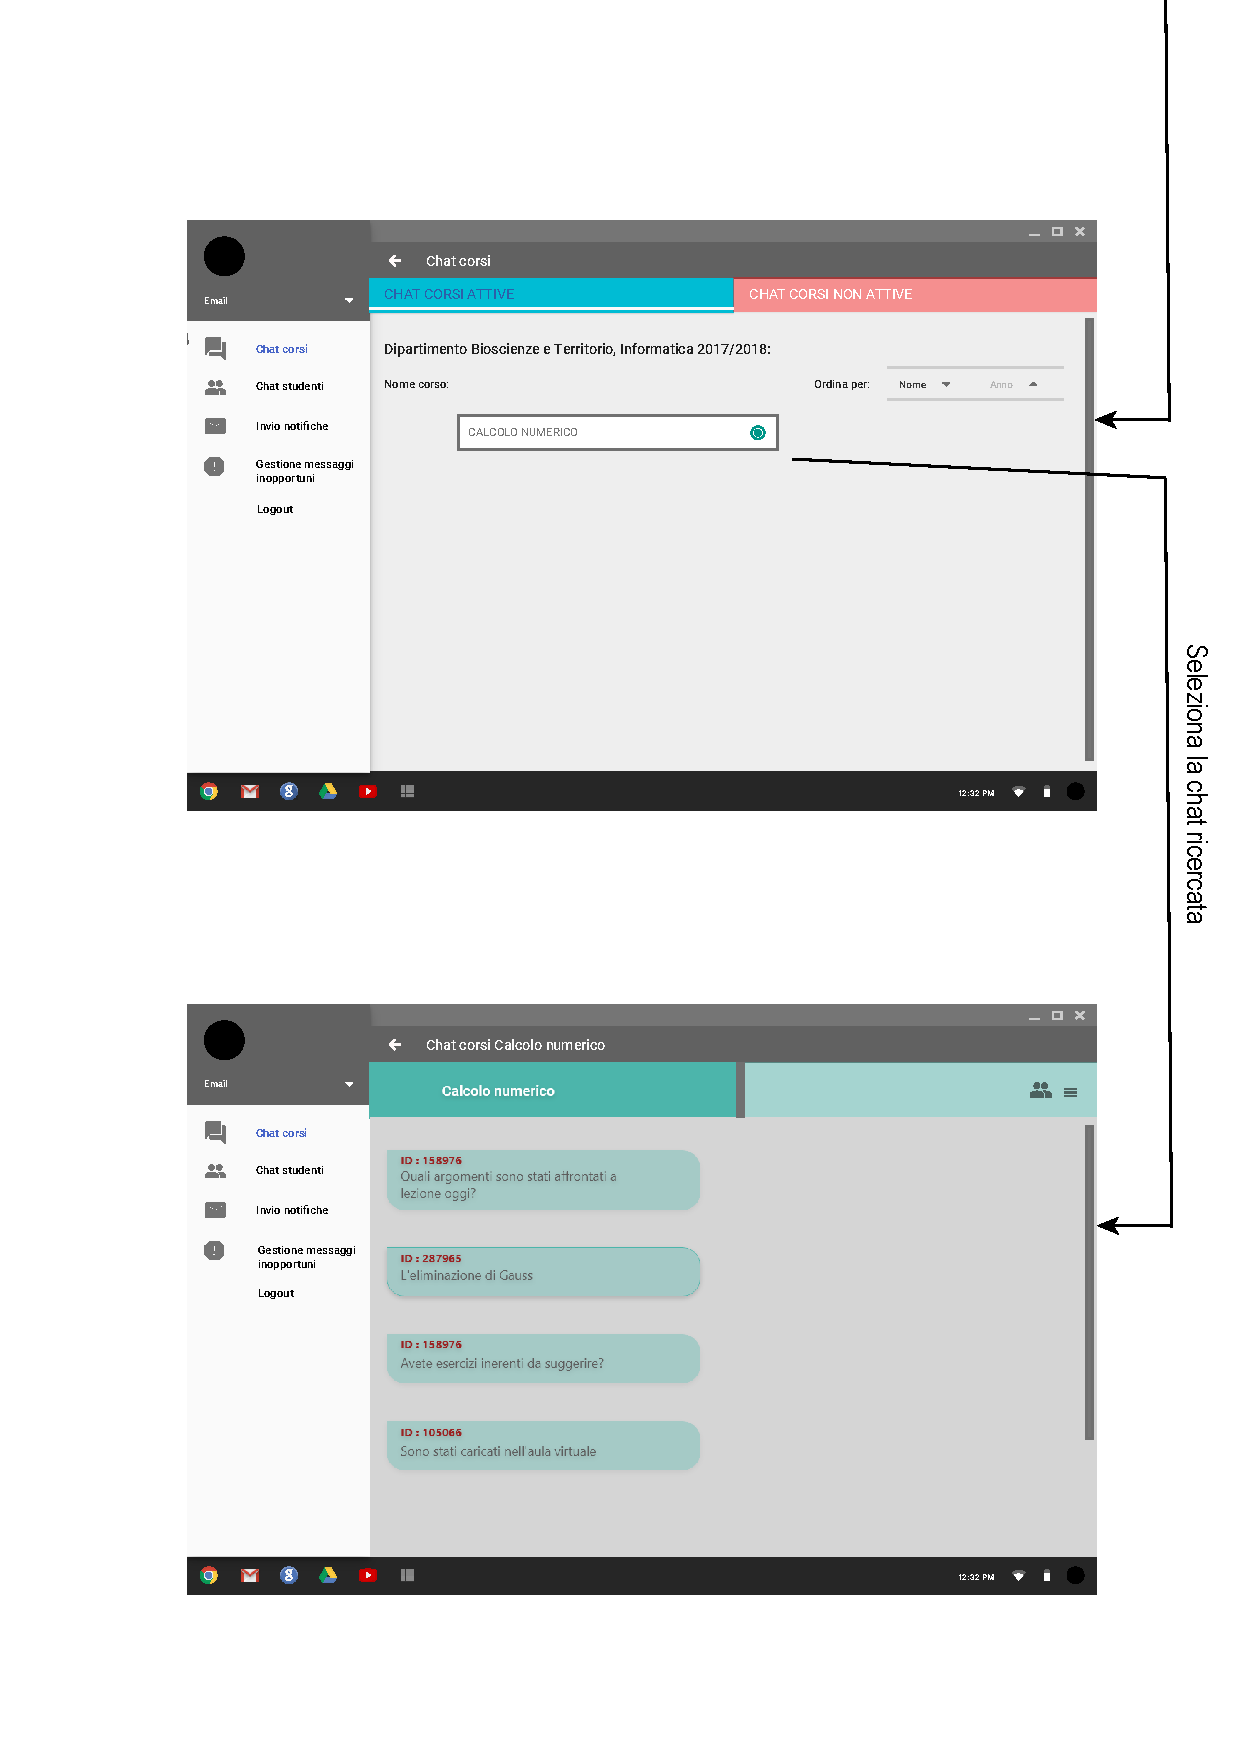
\includegraphics[width=0.9\textwidth]{imgs/gruppo6/activities/act_cup3_ricerca_chat_corsi2.pdf}
	\caption{CUP3 - Ricerca chat (cerca corsi - pt.2)}
	\label{fig:cup3-6}
\end{figure}

\begin{figure}
	\centering
	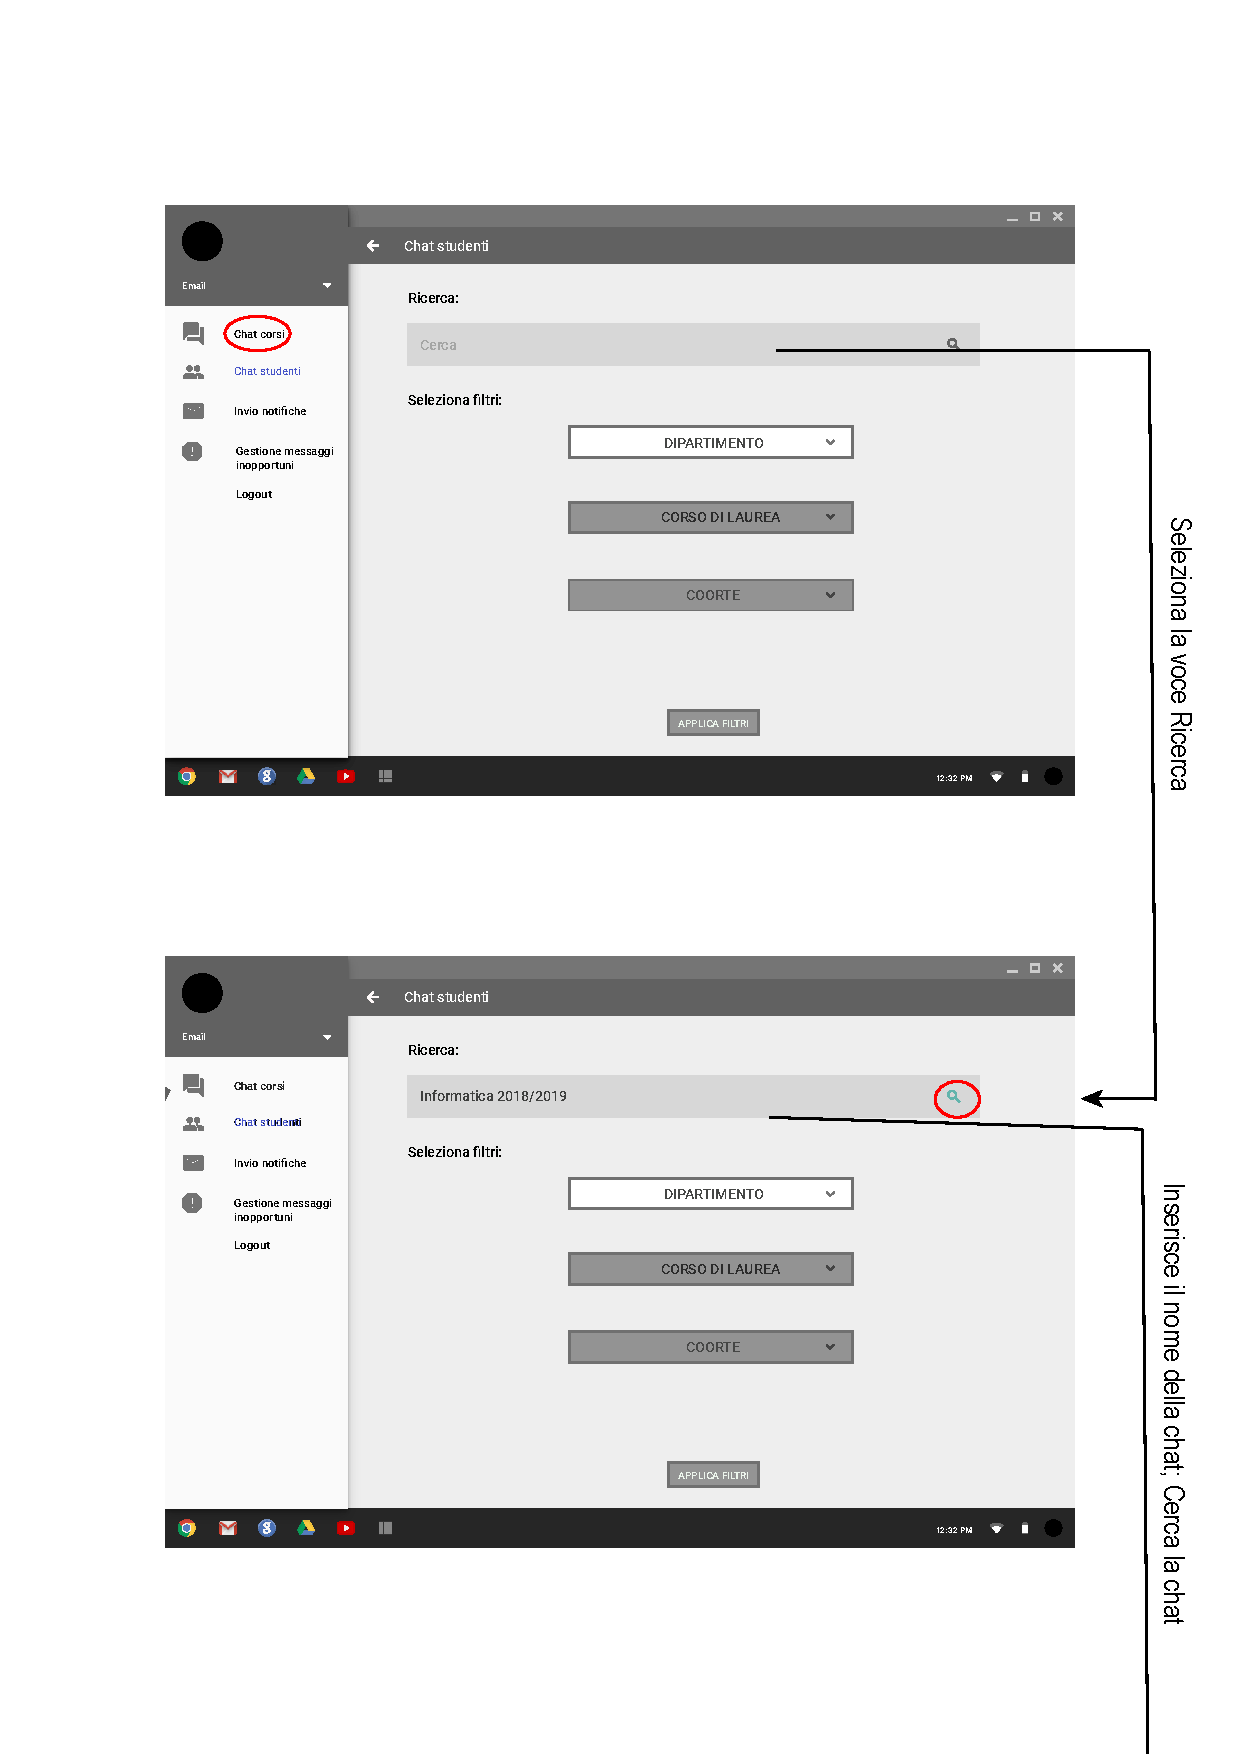
\includegraphics[width=0.9\textwidth]{imgs/gruppo6/activities/act_cup3_ricerca_chat_studenti.pdf}
	\caption{CUP3 - Ricerca chat (cerca studenti - pt.1)}
	\label{fig:cup3-7}
\end{figure}

\begin{figure}
	\centering
	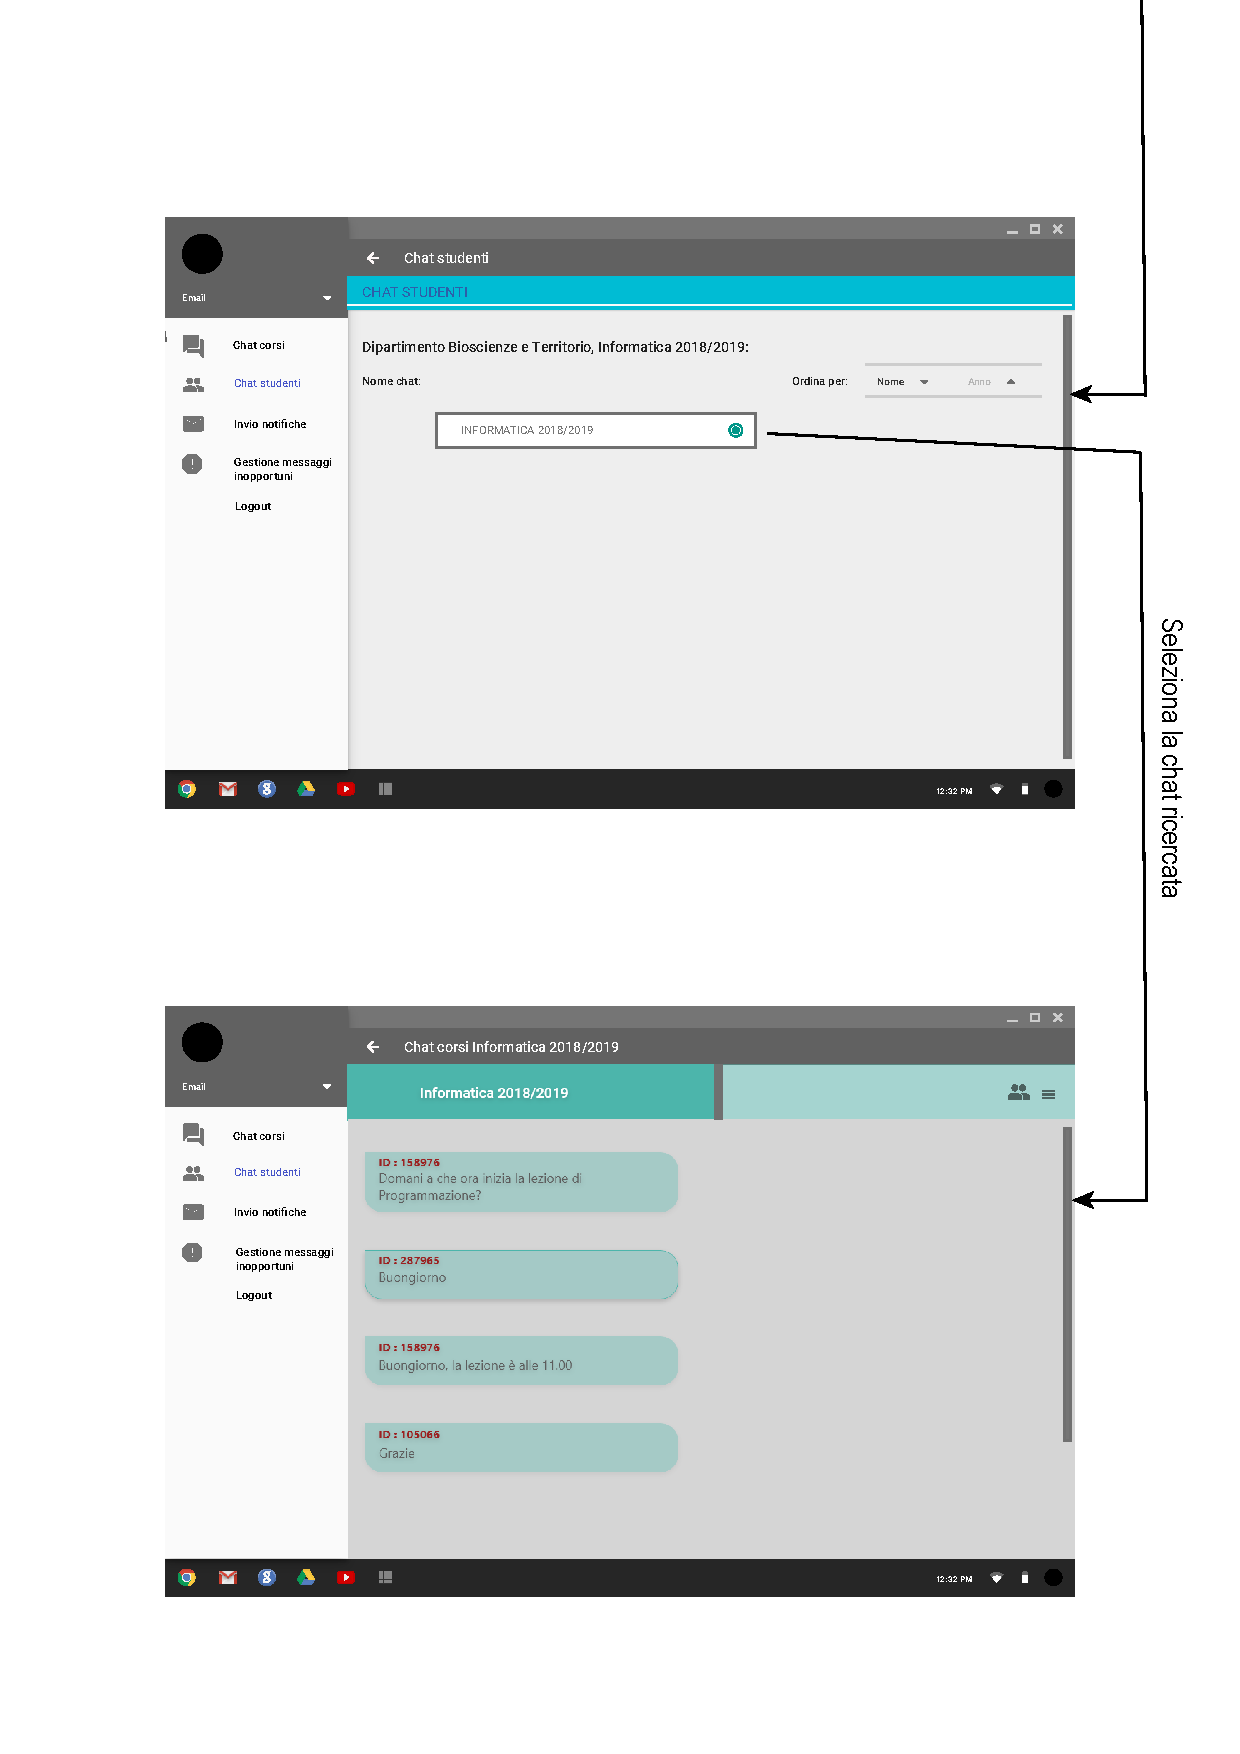
\includegraphics[width=0.9\textwidth]{imgs/gruppo6/activities/act_cup3_ricerca_chat_studenti2.pdf}
	\caption{CUP3 - Ricerca chat (cerca studenti - pt.2)}
	\label{fig:cup3-8}
\end{figure}

\begin{figure}
	\centering
	\includegraphics[width=0.9\textwidth]{imgs/gruppo6/activities/act_cup4_visualizza_lista_chat_corsi1.pdf}
	\caption{CUP4 - Visualizza lista chat (corsi - pt.1)}
	\label{fig:cup4}
\end{figure}

\begin{figure}
	\centering
	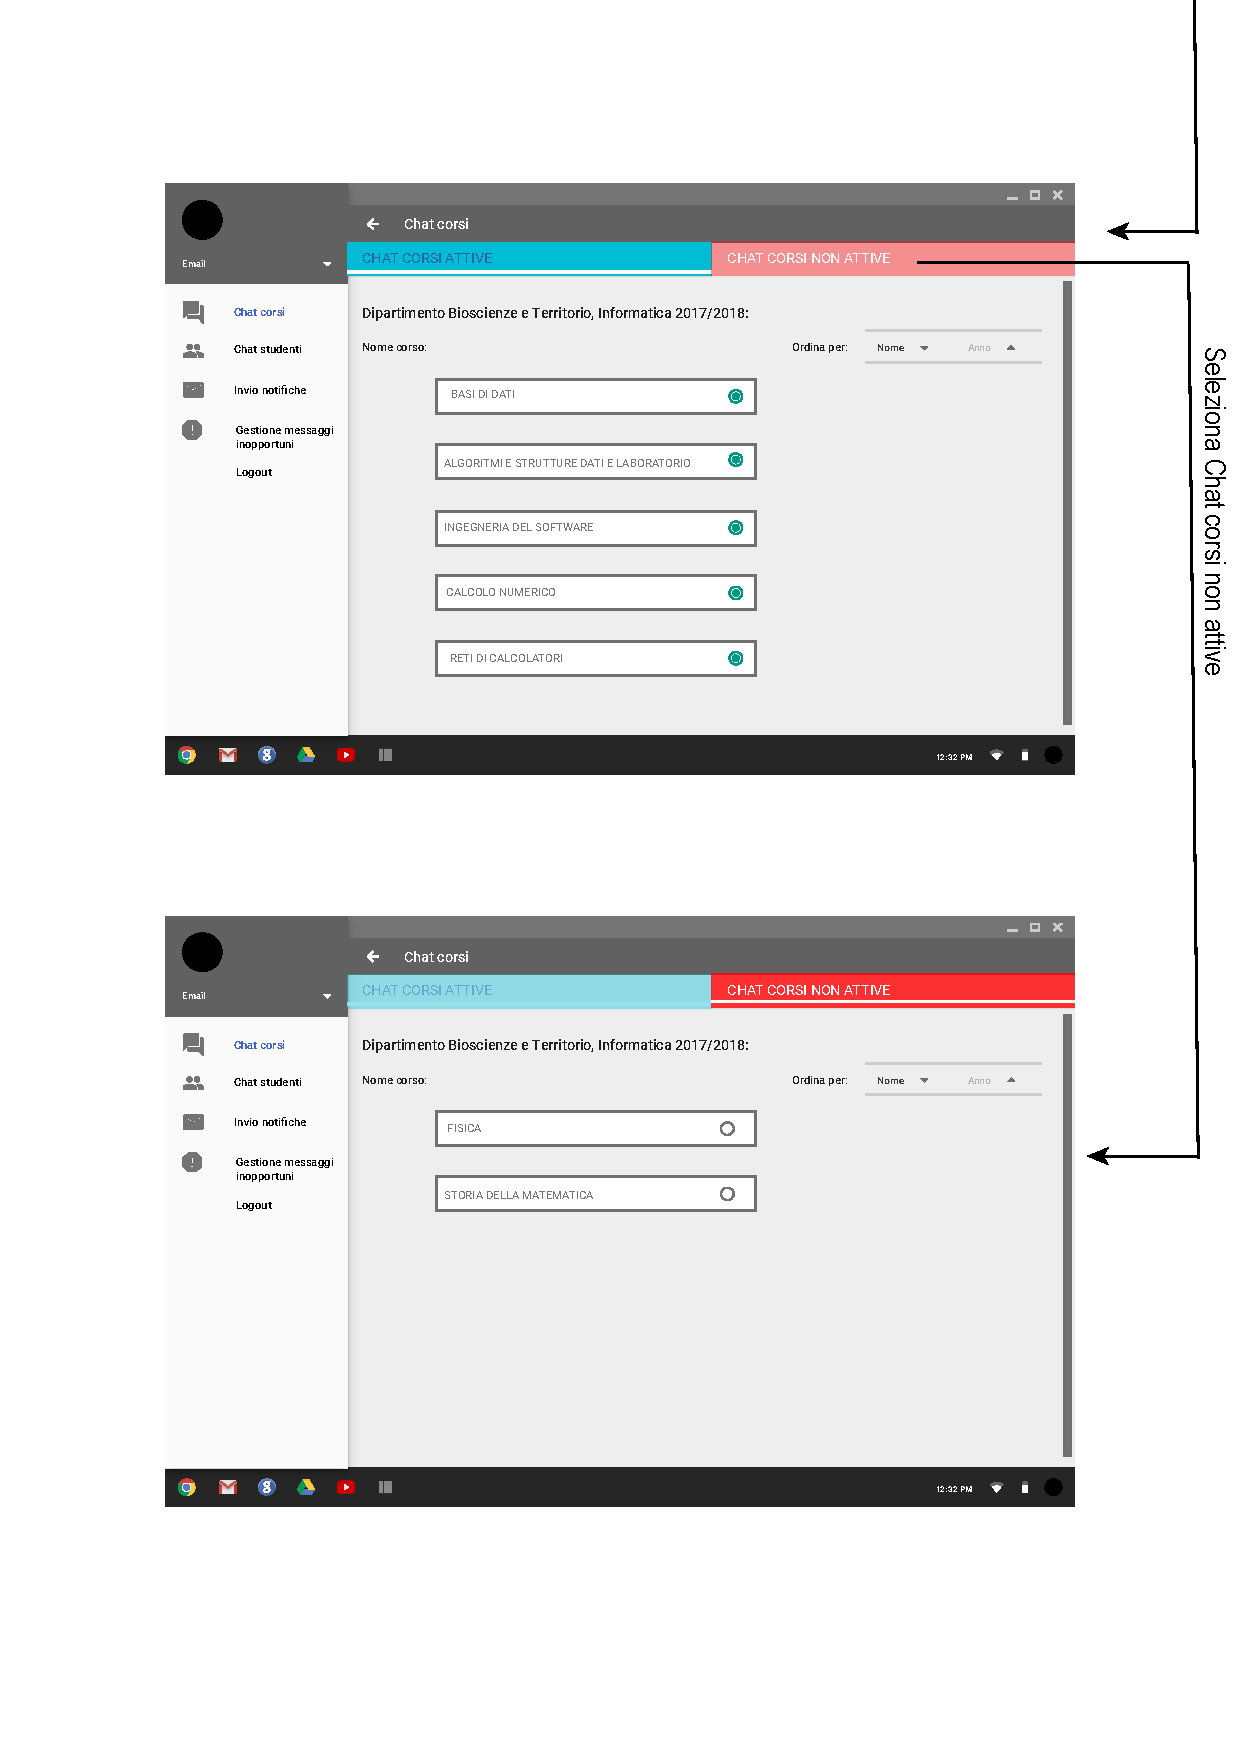
\includegraphics[width=0.9\textwidth]{imgs/gruppo6/activities/act_cup4_visualizza_lista_chat_corsi2.pdf}
	\caption{CUP4 - Visualizza lista chat (corsi - pt.2)}
	\label{fig:cup4-2}
\end{figure}

\begin{figure}
	\centering
	\includegraphics[width=0.9\textwidth]{imgs/gruppo6/activities/act_cup4_visualizza_lista_chat_studenti.pdf}
	\caption{CUP4 - Visualizza lista chat (studenti)}
	\label{fig:cup4-3}
\end{figure}

\begin{figure}
	\centering
	\includegraphics[width=0.9\textwidth]{imgs/gruppo6/activities/act_cup5_abilita_chat.pdf}
	\caption{CUP5 - Abilita chat}
	\label{fig:cup5}
\end{figure}

\begin{figure}
	\centering
	\includegraphics[width=0.9\textwidth]{imgs/gruppo6/activities/act_cup6_disabilita_chat.pdf}
	\caption{CUP6 - Disabilita chat}
	\label{fig:cup6}
\end{figure}

\begin{figure}
	\centering
	\includegraphics[width=0.9\textwidth]{imgs/gruppo6/activities/act_cup7_visualizza_canale.pdf}
	\caption{CUP7 - Visualizza canale}
	\label{fig:cup7}
\end{figure}

\begin{figure}
	\centering
	\includegraphics[width=0.9\textwidth]{imgs/gruppo6/activities/act_cup8_aggiungi_canale1.pdf}
	\caption{CUP8 - Aggiungi canale (pt.1)}
	\label{fig:cup8}
\end{figure}

\begin{figure}
	\centering
	\includegraphics[width=0.9\textwidth]{imgs/gruppo6/activities/act_cup8_aggiungi_canale2.pdf}
	\caption{CUP8 - Aggiungi canale (pt.2)}
	\label{fig:cup8-2}
\end{figure}

\begin{figure}
	\centering
	\includegraphics[width=0.9\textwidth]{imgs/gruppo6/activities/act_cup9_cancella_canale1.pdf}
	\caption{CUP9 - Cancella canale (pt.1)}
	\label{fig:cup9}
\end{figure}

\begin{figure}
	\centering
	\includegraphics[width=0.9\textwidth]{imgs/gruppo6/activities/act_cup9_cancella_canale2.pdf}
	\caption{CUP9 - Cancella canale (pt.2)}
	\label{fig:cup9-2}
\end{figure}

\begin{figure}
	\centering
	\includegraphics[width=0.9\textwidth]{imgs/gruppo6/activities/act_cup10_visualizza_lista_utenti.pdf}
	\caption{CUP10 - Visualizza lista utenti}
	\label{fig:cup10}
\end{figure}

\begin{figure}
	\centering
	\includegraphics[width=0.9\textwidth]{imgs/gruppo6/activities/act_cup11_aggiungi_utente_canale1.pdf}
	\caption{CUP11 - Aggiungi un utente ad un canale (pt.1)}
	\label{fig:cup11}
\end{figure}

\begin{figure}
	\centering
	\includegraphics[width=0.9\textwidth]{imgs/gruppo6/activities/act_cup11_aggiungi_utente_canale2.pdf}
	\caption{CUP11 - Aggiungi un utente ad un canale (pt.2)}
	\label{fig:cup11-2}
\end{figure}

\begin{figure}
	\centering
	\includegraphics[width=0.9\textwidth]{imgs/gruppo6/activities/act_cup12_cancella_utente_canale.pdf}
	\caption{CUP12 - Rimuovere un utente da un canale}
	\label{fig:cup12}
\end{figure}

\begin{figure}
	\centering
	\includegraphics[width=0.9\textwidth]{imgs/gruppo6/activities/act_cup13_silenziare_utente1.pdf}
	\caption{CUP13 - Silenziare utente in un canale (pt.1)}
	\label{fig:cup13}
\end{figure}

\begin{figure}
	\centering
	\includegraphics[width=0.9\textwidth]{imgs/gruppo6/activities/act_cup13_silenziare_utente2.pdf}
	\caption{CUP13 - Silenziare utente in un canale (pt.2)}
	\label{fig:cup13-2}
\end{figure}

\begin{figure}
	\centering
	\includegraphics[width=0.9\textwidth]{imgs/gruppo6/activities/act_cup14_reintegra_utente.pdf}
	\caption{CUP14 - Reintegra utente in un canale}
	\label{fig:cup14}
\end{figure}

\begin{figure}
	\centering
	\includegraphics[width=0.9\textwidth]{imgs/gruppo6/activities/act_cup15_modifica_permessi_utente1.pdf}
	\caption{CUP15 - Modificare i permessi di un utente in un canale (pt.1)}
	\label{fig:cup15-2}
\end{figure}

\begin{figure}
	\centering
	\includegraphics[width=0.9\textwidth]{imgs/gruppo6/activities/act_cup15_modifica_permessi_utente2.pdf}
	\caption{CUP15 - Modificare i permessi di un utente in un canale (pt.2)}
	\label{fig:cup15-2}
\end{figure}

\begin{figure}
	\centering
	\includegraphics[width=0.9\textwidth]{imgs/gruppo6/activities/act_cup16_nascondi_messaggio.pdf}
	\caption{CUP16 - Nascondi messaggio}
	\label{fig:cup16}
\end{figure}

\begin{figure}
	\centering
	\includegraphics[width=0.9\textwidth]{imgs/gruppo6/activities/act_cup17_reintegra_messaggio.pdf}
	\caption{CUP17  - Reintegra messaggio}
	\label{fig:cup17}
\end{figure}

\begin{figure}
	\centering
	\includegraphics[width=0.9\textwidth]{imgs/gruppo6/activities/act_cup18_invio_notifiche1.pdf}
	\caption{CUP18 - Invio Notifiche (pt.1)}
	\label{fig:cup18}
\end{figure}

\begin{figure}
	\centering
	\includegraphics[width=0.9\textwidth]{imgs/gruppo6/activities/act_cup18_invio_notifiche2.pdf}
	\caption{CUP18 - Invio Notifiche (pt.2)}
	\label{fig:cup18-2}
\end{figure}

\begin{figure}
	\centering
	\includegraphics[width=0.9\textwidth]{imgs/gruppo6/activities/act_cup19_gestione_messaggi_inopportuni.pdf}
	\caption{CUP19 - Gestione messaggi inopportuni}
	\label{fig:cup19}
\end{figure}
%%% END activities chat pannello %%%
\clearpage

\end{document}

%%%%%%%%%%%%%%%%%%%%%%%%%%%%%%%%%%%%%%%%%%%%%%%%%%%%%%%%%%%
